% !Mode:: "TeX:UTF-8"
\chapter{Introduction}

Nowadays there are many existing image compression approaches. We can divide such algorithms in two groups: lossy (such as JPEG. Mainly such algorithms use Discrete Cosine Transform) and lossless (such as DEFLATE. Mainly such algorithms use similar to Huffman Encoding methods). Both have been developed for decades already. It is important to mention that image containers (such as JPEG, PNG, GIF etc.) are using information compression algorithms \textit{only as a part} of their architecture. Usually lossy and lossless compression methods are combined to achieve higher performance.

The contribution of this work can be considered from two major perspective. The first is that this work is the first approach to use image enhancement approaches in decoder architecture. From the second perspective we use a general autoencoder architecture together with compression and coding algorithms. And finally we design a model that is customizable and can be further more improved in the future with advances in the field of image enhancement, information coding and image compression.

\section{Niches}

This work can improve existing image compression algorithms. The disk space required to store images compressed with the model should less than disk space required to store raw images or even images compressed with JPEG or JPEG2000. Such an algorithm can be used in different scenarios. Mainly we can use it in traditional use cases for lossy compression such as using it in image format as it is or in more advance sense, to extend existing formats. For example we can extend existing DCT (Discrete Cosine Transform) or DWT (Discrete Wavelet Transform). We selected two possible use cases to apply the compression algorithm we are developing:

\begin{enumerate}
    \item Limited space on machine with high computational power. It can be a big server with powerful CPU. In recent days there are some movements in quantum computing sphere, so it can be a very powerful machine with quantum CPU etc.
    \item Huge images needed to be transmitted through a network with limited speed. In case of a limited performance of a network we can compress and restore images using application, we are working on.
\end{enumerate}

Few years ago already a reasonable performance has been achieved using an encoder-decoder architecture \cite{theis_lossy_2017}. We suppose, that our approach can boost performance both in sense of visual appearance and sense of compressed image size.

\section{Image compression}

JPEG is widely used in image compression applications. It was introduced in 1992 \cite{wallace_jpeg_1992}. Algorithm consists of several steps. The first step is transformation from RGB color space to YCbCr color space (Chroma subsampling). The next step is Discrete Cosine Transform (DCT), a special transformation which is based on Fourier Transform, this step is lossless. After DCT goes Quantization, the only lossy step of JPEG image compression standard. The last step of compression is Coding, which only encodes symbols sequencies to more efficient in terms of occupied space format, this step is lossless.

There is a certain trend to apply a power of neural networks in compression domain, extending a group of lossy algorithms. First approaches were \cite{himentzer_high_fidelity_2020 Balle_Laparra_Simoncelli_2017, theis_lossy_2017, Toderici_Vincent_Johnston_Hwang_Minnen_Shor_Covell_2017}, where authors proved that it is possible to use one neural network to generate a compressed representation of an image and another neural network to restore initial image from its representation generated by first network. Now such networks are also being used to solve an image and video upscale tasks.

Recent progress in neural image compression has shown a great progress. Now neural image compression outperform traditional compression algorithms such as JPEG and JPEG2000 and development of convolutional layers architecture provides a more powerful tools to extract image features and reconstruct initial image.

However, several issues are still remaining unsolved:

\begin{enumerate}
    \item False textures.
    \item Limited compression power.
    \item Large model size.
    \item Noise artifacts.
\end{enumerate}

For now a general approach is to encode an image to a compressed representation using convolutional neural network and take the convolutional features from one of the top layers of network. Then these features can be stored and later with the use of another convolutional neural network that employs deconvolution the initial image can be obtained.

In this work we are going to apply fully convolutional neural network to extract features from given image, afterwards we compress those features using another encoder and arithmetic coding algorithm. Then this compressed representation is restored using decoder and upsample modules. It worth to mention that the algorithm we are working on is lossy. Our method will combine traditional image compression approaches and neural network image compression approach.

\section{Objective}

Our motivation is that traditional image compression methods are simple and computationally efficient. However, using more heavy neural models we can compress image much more efficient. By combining these two methods we can reach equilibrium.

Nowadays existing methods have a strong compression power. Existing models significantly overcome traditional methods by many metrics. The most impressive though is a PSNR metrics, which measures an effectiveness of compression.

In this work our objective is to improve existing techniques in image compression domain: we build a model that is capable of compressing images in efficient way, the compressed images should take less disk space than existing models; our model need to outperform existing models in terms of reconstructed images quality; we also plan to reduce the size of the compression model to find an optimal number of parameters in generator.

\section{Research content}

To conduct this research we started from studies in the field of image compression. We have completed reading of papers related to the subject and selected the most suitable ones for this work. We trained them separately and compared the performance of the models. To do this we made a research on neural networks training pipeline, where we cover the basic neural network training algorithms, advanced techniques and the most efficient algorithms which are used nowadays. We show the continuity of development for neural networks training algorithms starting from famous gradient descent and ending by Adam. In our work we use autoencoder architecture, thus we describe the architecture design and training pipeline of autoencoder based models. We include all the necessary equations and formulas for understanding the autoencoders. We also use generative adversarial networks in our thesis, and describe how the GAN can improve image compression and make compression algorithm more accurate. We describe training pipeline of GAN models and provide all the formulas used for building GAN. In our networks we use a special convolutional architecture and modern channel normalization.

This work is based on two components: autoencoder and GAN. In following sections we show in details our model architecture and describe its' joint training pipeline from the beginning up to the end.

We show the result of proposed architecture and list the modules that were used as a base for our model. Analysis of the results confirms that our method performs better on used metrics.

\section{Organization of the thesis}

In this work we are going to give a deep review of existing methods of image compression including modern and traditional approaches. In the chapter \nameref{chapter:literature} we review the existing approaches in neural image processing in general and neural image compression in particular.

In the chapter \nameref{chapter:methodology} we in deep describe the architecture of our model. We provide the necessary formulations of the modules we use in our work, such as Autoencoder model, GAN model and algorithms such as Huffman coding and arithmetic coding. I this chapter we also describe the training pipeline including two parts: compression autoencoder model training, GAN training and fine tuning with the image enhancement models.

In our \nameref{chapter:experiments} chapter we describe our experiments. We start this chapter with the introduction of datasets we use in the experiments. Next we describe the way we train our model including the algorithms, hyperparameter settings, we show the behaviors of the loss functions during the training. Next we introduce the evaluation process and show the result images. In evaluation section we describe the metrics we are using and show that our model outperforms the baseline model. We select the best image enhancer and show that it improves the images quality.

\chapter{Literature review}
\label{chapter:literature}

Convolutional neural networks have shown a high performance in a variety of tasks during recent decade. Power of convolutional neural networks (CNNs) is mainly due to their ability to aggregate and generalize local features. It turns out that CNN architecture is extremely good and effective when we deal with \textit{structured data}. In early beginning of CNNs milestone works were VGG-19 \cite{simonyan_very_2015} and AlexNet \cite{alexnet}, where authors proved that convolutional architectures can be way more computationally effective than we thought before. It has also been shown that learned convolutional filters can reflect a local structure of sample.

Nowadays CNNs are used in a variety of tasks such as classification,  image generation, clustering, dimensionality reduction etc. One of possible applications of CNN is neural image compression. In neural image compression we use a compression power of convolutional neural network, which is a stack of convolutional layers, such as \cite{alexnet}.

\section{Preliminary and background}

Image compression has a several conventional steps, which are usually employed in neural image compression too. These steps are well described in \cite{JPEG-1992}. JPEG standard was introduced in 1992 and adopted as an image compression standard by Joint Photography Expert Group. JPEG has a module structure, so these modules implementation can be changed drastically, while having same interaction with other modules. This helps to replace an old modules by more advanced and modern ones. For example, Huffman Coding \cite{Huffman-Coding} in Coding stage of JPEG algorithm can be replaced by Arithmetic coding \cite{Arithmetic-Coding}. Many papers employ this module structure, so authors can use already existing ones and only work on one part of the whole compression algorithm to further improve exactly the part they are interested in.

To understand main neural image compression approaches, we need to get familiar with autoencoder architecture first. First time introduced in 2006 \cite{Autoencoder_2006}. In this paper authors propose an unusual method to reduce a dimensionality of data: use neural network build up from two components, encoder and decoder. They significantly overcome efficiency of Principal component analysis \cite{pca} in dimensionality reduction. Dimensionality reduction late has become a closely related to neural image compression. Autoencoder consists of two very specific for its' architecture parts: Encoder and Decoder. In the original paper they have (2-4) hidden layers in the encoder and decoder, but now modern approaches can be much more deep. A main principle of autoencoder is that we use encoder to reduce dimensionality (this results to some kind of data compression, and in other words with the help of encoder we compress data to some compact representation). Afterwards we use Decoder to reconstruct data from intermediate representation to it's original shape. Both encoder and decoder are multilayer neural networks, which makes it extremely flexible and open to all the machine learning progress we have and potentially will have in the future. To train such a model we need to initialize these two networks and propagate the information through encoder and decoder sequentially. Then we need to calculate an error. Decoder output has the same shape as the original sample and usually we define loss as a distance from input sample to the decoder output (such as L1 or L2 distances). Later we use any of existing optimizers perform a backpropagation this loss value and adjust weights.

\section{Methods for training neural networks}

Training of neural network is a process of iterative adjusting parameters of this network, which aims to minimize the loss function. Understanding training of neural networks is essential for successful training of the network. In this work we use Adam \cite{kingma_adam_2017} algorithm, but for clear understanding of Adam optimizer and right selection of its parameters we need to understand the algorithms Adam is based on. In the following subsections we cover these algorithms.

\subsection{Nesterov Accelerated Gradient}

The idea of momentum accumulation methods is obviously simple. If we are moving in a certain direction for some time, then we should probably move there for some time in the future. To do this, we need to have an access to the recent history of changes of each parameter. We can store the last $n$ instances of $\Delta W$ and calculate the average at each step, but this approach takes up too much memory for large $n$. Fortunately, we do not need an exact average, but only an estimate, so we can use an exponential moving average.

\begin{equation}
    \label{eq:derivative-momentum-1}
    v_t = \gamma v_{t-1} + (1-\gamma) x
\end{equation}

To accumulate we are going to multiply already accumulated value by the factor $0 < \gamma < 1$ and add another value multiplied by $1-\gamma$. The closer $\gamma$ is to $1$, the larger the accumulation window and the stronger the smoothing — the history of $x$ influences more strongly than each successive $x$. If $x=0$ from some point, $v_t$ fade exponentially. We apply an exponential running average to accumulate the gradient of the objective function of a network:

\begin{equation}
    v_t = \gamma v_{t-1} + \eta \nabla_W J(W)
\end{equation}

And update weights:

\begin{equation}
    W = W - v_t
\end{equation}

Where $\gamma$ is usually of the order $0.9$. Note that $1-\gamma$ is not missing, but included in $\eta$. The smaller the $\gamma$, the more the algorithm behaves like a regular SGD. To get a popular physical interpretation of the equations, we can imagine a ball rolling on a hilly surface. If at the moment $t$ there was a non-zero slope under the ball ($\nabla_W J(W)$), and when it hit a plateau, it will still continue rolling along this plateau. Moreover, the ball will continue to move a couple of updates in the same direction, even if the slope has changed to the opposite. Nevertheless every second it loses $1-\gamma$ of its speed.

Note that accumulated value $v_t$ may very much exceed the value of each $\eta\nabla_W J(W)$. A simple accumulation of momentum already gives a good result, but Nesterov goes further and applies a well-known idea from calculus: looking ahead along the update vector. Since we are going to shift to $\gamma v_{t-1}$ anyway, let's calculate the gradient of the loss function not at the point $W$, but at $W - \gamma v_{t-1}$.

\begin{equation}
    v_t = \gamma v_{t-1} + \eta \nabla_W J( W - \gamma v_{t-1} )
\end{equation}

\begin{equation}
    W = W - v_t
\end{equation}

Such a change fores loss to decay faster, if in the direction we are moving derivative is increasing, and slower, if opposite.

\subsection{Adagrad}

Some features can be very informative. It could happen that we have a pattern that only after few convolutional layers becomes a significant feature.. It would be great being able to update parameter with regard to its' feature change. It's not a difficult one, we just should store for a parameter a sum of squares of its' updates. It will stand for similarity: if the parameter belongs to a chain of frequently activated neurons, the sum is accumulating fast.

\begin{equation}
    G_{t} = G_{t} + g_{t}^2
\end{equation}

\begin{equation}
    W_{t+1} = W_{t} - \frac{\eta}{\sqrt{G_{t} + \epsilon}} g_{t}
\end{equation}

Where $G_{t}$ is a sum of squares, аn $\epsilon$ is a smoothing parameter required to avoid division by $0$. If parameter updates frequently then $G_t$ is high and divisor is also big. $\epsilon$ is usually of order $10^{-6}$ or $10^{-8}$ for really aggressive updates, but it only plays a role in the beginning, near the middle $g_t$ starts to overcome $G_t$:

Main idea of Adgrad \cite{adgrad} is to use a mechanism to update frequently updated parameters less. Also, this formula is not the only one. Actually Adgrad is a family of algorithms, for example we can remove square root or store abs values of updates. Basically using Adgrad we automatically get so called learning rate decay.

\subsection{RMSProp и Adadelta}

Disadvantage of Adagrad is that $G_{t}$ could increase without any limit, and some time later it can stagnate. RMSProp and Adadelta \cite{adadelta} are to overcome this disadvantage. To acheave this we still update parameters based on theirs update history. But instead of full sum of updates we can use an averaged square of gradient.

\begin{equation}
    E[g^2]_t = \gamma E[g^2]_{t-1} + (1 - \gamma) g^2_t
\end{equation}

Then we get

\begin{equation}
    W_{t+1} = W_{t} - \frac{\eta}{\sqrt{E[g^2]_t + \epsilon}} g_{t}
\end{equation}

Divisor is a square root from gradient squares mean, thus RMSProp — root mean square propagation

\begin{equation}
    RMS[g]_t = \sqrt {E[g^2]_t + \epsilon }
\end{equation}

Adadelta differs from RMSProp by numerator, which uses $RMS$ from $\Delta W_t$. On step $t$ we do not know $RMS[\Delta W]_{t}$.

\begin{equation}
    \Delta W = -\frac{RMS[\Delta W]_{t-1}}{RMS[g]_{t}}g_{t}
\end{equation}

\begin{equation}
    W_{t+1} = W_{t} - \frac{RMS[\Delta W]_{t-1}}{RMS[g]_{t}}g_{t}
\end{equation}

\begin{equation}
    E[\Delta W^2]_t = \gamma E[\Delta W^2]_{t-1} + (1 - \gamma) \Delta W^2_t
\end{equation}

\begin{equation}
    RMS[\Delta W]_{t} = \sqrt{E[\Delta W^2]_t + \epsilon}
\end{equation}

Note that we need $RMS[\Delta W]_{-1}$ to be $0$ for the first step, all the following $\Delta W$ and $RMS[\Delta W]_{t}$ are going to be $0$. that's why we need $RMS \epsilon$. For RMSProp and Adadelta and Adagrad we don't have to set parameters precisely. Usually it's good to start $\eta$ with $0.1 - 1$, and $\gamma$ with $0.9$.

\subsection{Adam}

Adam \cite{kingma_adam_2017} — adaptive moment estimation, yet another optimization algorithm. It combines an idea of value accumulation and an idea of Adgrad and RMSProp.

\begin{equation}
    m_t = \beta_1 m_{t-1} + (1 - \beta_1) g_t
\end{equation}

Unlike Nesterov we accumulate not $\Delta W$, but the values of the gradient though this is kind of a cosmetic change. Besides, we want to know how frequent does the gradient change. Authors of Adam purposed to measure mean variance:

\begin{equation}
    v_t = \beta_2 v_{t-1} + (1 - \beta_2) g_t^2
\end{equation}

It's easy to find that $E[g^2]_t$ is the same in RMSProp.

An important difference from RMSProp is in initial adjusting of $m_t$ and $v_t$: they suffer from the same problem as $E[g^2]_t$ from RMSProp: in case of starting value is $0$ it will take many iterations to calibrate especially with a big window of accumulation ($0 \ll \beta_1 < 1, 0 \ll \beta_2 < 1$). This can be solved by introducing two new hyperparameters, but there is another way: artificially increase $m_t$ and $v_t$ on the first steps ($0 < t < 10$ for $m_t$ and $0 < t < 1000$ for $v_t$)

\begin{equation}
    \hat{m}_t = \frac{m_t}{1 - \beta^t_1}, \;
    \hat{v}_t = \frac{v_t}{1 - \beta^t_2}
\end{equation}

Finally rule of update:

\begin{equation}
    W_{t+1} = W_{t} - \dfrac{\eta}{\sqrt{\hat{v}_t + \epsilon}} \hat{m}_t
\end{equation}

Adam authors suggest to use following default values: $\beta_1 = 0.9$, $\beta_2 = 0.999$, $\epsilon = 10^{-8}$ and claim that the algorithm performs better or at least not worse than previous algorithms of optimization.

\section{Neural image processing}

Neural image compression usually follows an autoencoder pipeline.

\subsection{Fully convolutional neural networks in image processing}

Fully convolutional neural network is a type of neural network without an aggregate layer. Usually such an aggregation operation is a pooling. Pooling layer mechanics is simple: we need some functions that is a permutation invariant, so, it can make a generalization. This function for example can be a min, max, sum or average. These functions are irreversible, so we can not find a reverse function. Since conceptually decoder of an autoencoder is basically a reverse function for an encoder, we need something like this. The compression process must be reversible, otherwise we can not decompress an original image.

Fully convolutional neural networks is well-described in \cite{fcn}. Authors use fully convolutional network for semantic segmentation. Semantic segmentation is a special task in computer vision, where the final proposal is to label each pixel of image according to the object it belongs to. Traditionally this task is solved with clustering algorithms. The FCN (fully convolutional network) authors use is a network with only convolutional elements, this network only has a convolutional layers. Since convolutional layer architecture doesn't require a fixed-size input, it is extremely convenient to use these network with non-fixed size input data.

Each input for convolutional layer is a tensor of size $H \times W \times D$, where $H$ and $W$ are spatial dimensions and $D$ is depth dimension. Each next layer is connected to certain area in the previous layers and the more deep we go through the network the bigger is this area. This area is called a \textit{receptive field}. Convolutional neural networks are translation invariant. Components FCNs are build up with are pooling layers, convolutional layers and activation functions operate on local receptive fields, some regions of input data. Formula can be seen in equation \ref{eq:fcn-1}

\begin{equation}
    \label{eq:fcn-1}
    y_{ij} = f_{ks}(\{ x_{si + \delta i, sj + \delta j} \}_{0 \le \delta i, \delta j \le k})
\end{equation}

Where $k$ is a kernel size, $s$ is stride and $f$ is layer type.

A real-valued loss function defines a task. As well as in many other machine learning models, we use loss function as a start for backpropagation process. So, next we can use any of existing optimizers to converge network to its' local minima.

\subsection{Neural image enhancement}

Neural image enhancement is yet another application of autoencoders in neural image processing. Neural image enhancement models are designed to enhance images quality. Enhancer networks are used in image and video debluring, upscaling, denoising. The core of these methods is autoencoder architecture and ideas from here are widely used in neural image compression methods, that will be mentioned in the next section.

One of the most popular model for image enhancement is U-Net \cite{ronneberger_u-net_2015}. U-net is a convolutional autoencoder with encoder and decoder models, but it also has skip connections: some outputs of encoder are connected with skip-connections to corresponding decoder outputs. This type of model is highly capable of enhancing images while keeping its' main features and structure.

In \cite{odena_deconvolution_2016} authors claim checkerboard artifacts to be a significant drawback while processing a bright images. \textit{Checkerboard artifacts} are a special artifacts that appear on synthetically generated images, received from neural network. These artifacts are due to deconvolution nature: while performing a deconvolution the output of each patch in deconvolution layer ha an overlap with other patches outputs, tis leads to highly contrast artifacts similar to white-black checkerboard structure. Authors claim that this situation happens in many researches \cite{dumoulin_adversarially_2017,donahue_adversarial_2017,salimans_improved_2016,radford_unsupervised_2016}. They propose several approaches to overcome this issue: one approach is to make sure that kernel size is divided by the stride is used, another approach is to separate out an upsampling from lower to higher resolution and convolution (for example we can first use interpolation to roughly upscale an image and then apply a convolution). Conceptually they state that deconvolution operation can be separated into two operations mentioned above and this can help to reduce checkerboard artifacts.

In \cite{ehrlich_quantization_2020} they propose a mechanism of enhancement based on quantization table and YCbCr channels neural processing. JPEG \cite{JPEG-1992} luminance channel is twice bigger than Cb and Cr channels. Authors first enhance luminance channel and only then enhance Cb and Cr channels. They do it this way because luminance channel can be used in Cb and Cr channels, since their structure is similar within one image. So, the pipeline they propose has several steps.Firstly they take quantization matrix, which the image was compressed with. This matrix is stored inside JPEG container, so we can have it as an input without any additional actions. Then the luminance channel and quantization matrix are being fed to neural network, that enhances luminance channel based on its' structure and quantization matrix. Having luminance channel enhanced they use it as an input to color channel correlation network, which is another enhancer for Cb and Cr - color channels.

In another paper \cite{li_learning_2020} authors use similar approach. The network architecture of the proposed method contains the restoration branch and the global branch. The restoration branch extracts local features and restores the compressed image. The global branch learns global features to improve the artifacts removal results. The global and local features are merged in the middle of the restoration branch and then follow up by several residual blocks.

\subsection{Autoencoder applications in image processing}

First time introduced in \cite{Toderici_Vincent_Johnston_Hwang_Minnen_Shor_Covell_2017}, convolutional neural compression employs an autoencoder architecture and some steps from traditional image compression pipeline. They optimize a tradeoff between a number of bits used to store data (based on symbol frequencies and called an \textit{entropy coding}) and distortion from equation \ref{eq:rate-distortion}.

\begin{equation}
    \label{eq:rate-distortion}
    − log_2 Q ([f (x)]) + \beta · d (x, g([f (x)]))
\end{equation}

Where $\beta$ is a hyperparameter that controls a rate-distortion tradeoff, $Q$ is compression rate and $d$ is distortion rate.

The first problem we encounter going through this problem is that quantization operation is not differentiable. Since quantization employs rounding, it is zero everywhere except integers, where it is undefined. Authors propose to use a smooth approximation for quantization during backward pass.

\begin{equation}
    \label{eq:quantization}
    \frac{d}{dy}[y]:=\frac{d}{dy}r(y)
\end{equation}

Where $r$ is an approximation function. For simplicity authors used $r(y)=y$, this makes the operation much more easy to implement. Gradients simply pass from the decoder to encoder.

Authors use elements from \cite{shi_real-time_2016}, basically employing such operations as convolution, residual blocks in the middle and sub-pixel convolutions in the decoder network.

In \cite{jiang_towards_2021} authors propose FBCNN for JPEG artifacts removal. FBCNN is also based on U-Net \cite{ronneberger_u-net_2015} and consists of four parts: encoder, quality factor predictor, flexible controller, and decoder. The encoder extracts the deep features from the input corrupted JPEG image and then splits them into image features and QF features which are subsequently fed into the decoder and predictor, respectively. The controller gets the estimated QF from the predictor and then generates QF embeddings. The QF attention block enables the controller to make the decoder produce different results according to different QF embeddings. The predicted quality factor can be changed with interactive selections to have a balance between artifacts removal and details preservation.

\subsection{Generative adversarial networks in image processing}

Generative adversarial networks (GANs) are neural networks, that are deigned to be trained in a special manner. Almost every existing network can be trained in adversarial manner, since the structure of the network itself doesn't change. Adversarial training uses same approaches as regular training, but with some modification: for adversarial training we need to construct a neural network that is capable of distinguishing between \textit{real} images (input images from dataset) and \textit{fake} ones (those, generated by the network). To train this model, we separate each iteration of training on two steps: firstly we pass input through general pipeline (without discriminator) and calculate loss, then we pass input through general pipeline and then feed this output to discriminator network. Then we can calculate discriminator loss and backpropagate.

GANs were first time introduced by \cite{Goodfellow_Pouget-Abadie_Mirza_Xu_Warde-Farley_Ozair_Courville_Bengio_2014}. They learn generator distribution $p_g$ over data $x$, they define a prior on input noise variables $p_z(z)$, then represent a mapping to data space as $G(z, \Theta_g)$, where $G$ is a differentiable function (neural network with parameters $\Theta_g$) They also define a second network $D(x, \Theta_d)$ that outputs a single scalar. $D(x)$ represents the probability that input $x$ came from the data rather than $p_g$. They train $D$ to maximize the probability of assigning the correct label to both training examples and samples from $G$. They simultaneously train $G$ to minimize $log(1 − D(G(z)))$ in equation \ref{eq:gan}:

\begin{equation}
    \label{eq:gan}
    min_G max_D V(D, G) = E_{x~p_{data}(x)} [log D(x)] + E_{z~p_z(z)} [log(1 - D(G(z)))]
\end{equation}

ESRGAN \cite{Wang_Yu_Wu_Gu_Liu_Dong_Qiao_Loy_2019} and RealESRGAN \cite{Wang_Xie_Dong_Shan_2021} are two similar papers where authors try to resolve the issue of image quality enhancement. More concrete, in those papers authors propose a model to perform a super-resolution.They use a common pipeline which has already widely spread among image super-resolution models. They use a convolution to map original image to lower spatial dimensional space, but higher channel dimensional space. Then they follow convolution by applying several residual blocks. This residual network doesn't change the data dimensionality and the number of residual blocks can vary over different variants of network. Then they upscale image with interpolation (different ones were used: bicubic, bilinear, Nearest-neighbor interpolation) followed by convolutions to reduce number of channels and increase spatial dimensions back to the initial state of 3. This model is trained in GAN manner, so Discriminator is used.

Recently a U-Net based discriminator was proposed in \cite{schonfeld_u-net_2021}. This U-Net discriminator classifies the input images on a global and local per-pixel level. Due to the skip-connections between the encoder and the decoder, the channels in the output layer contain both high-level and low-level information. Brighter colors in the decoder output correspond to the discriminator confidence of pixel being real (and darker of being fake). So the discriminator has a confidence map with size of the image. The discriminator consists of the original downsampling network and an upsampling network. The two modules are connected via a bottleneck, as well as skip-connections that copy and concatenate feature maps from the encoder and the decoder modules. Discriminator loss is described in equation \ref{eq:u-net-discriminator}.

\begin{equation}
    \label{eq:u-net-discriminator}
    \begin{split}
        L_D = -E_z[log D_{enc}^U(G(z)) + \sum_{i,j}{log [D_{dec}^U(G(z))]_{i,j}}]
    \end{split}
\end{equation}

Where $D_{enc}^U$ is an encoder part of the discriminator, $D_{dec}^U$ is a decoder part of the discriminator. The first term of this formula stands for distinguishing the whole picture to be fake or real and the second term stands for every pixel of an image to be fake or real. The second term generalize each pixel data of the generated fake/real confidence map by summing them up. In this formula $[D_{dec}^U(G(z))]_{i,j}$ refer to the discriminator decision at pixel $(i,j)$.

\section{Neural image compression}

In this section we will show that neural networks can also be used in image compression. As it was mentioned in the paper \cite{Autoencoder_2006}, autoencoders are a very powerful tool for reducing a dimensionality of data, which makes them a suitable choice for image compression. The task of image compression is to reduce the size of given image while keeping it's visual features. In other words the objective in image compression is to maximize the quality of compressed and decompressed image and minimize the number of bytes required to store the image.

One of the first approaches here has been described in \cite{Toderici_Vincent_Johnston_Hwang_Minnen_Shor_Covell_2017}. It was the first paper that has successfully outperformed JPEG. Each of the architectures they describe can provide variable compression rates during deployment without requiring retraining of the network: each network need only be trained once. The framework consists of three modules: encoder, binarizer and decoder. The structure of the framework is similar to \cite{Autoencoder_2006}: uncompressed image goes through encoder; then features with reduced dimensionality go to the binarizer and being compressed into binary codes, that can be stored on drive; those codes can also be transmitted to decoder, which creates an estimate of the original image based on the binary code.

A single iteration of their network can be represented using following formula \ref{eq:rnn-compression-1}:

\begin{equation}
    \label{eq:rnn-compression-1}
    \begin{split}
        b_t = B(E_t(r_{t-1})), \hat{x}_t = D_t(b_t) + \gamma \hat{x}_{t-1} \\
        r_t = x - \hat{x}_t, r_0 = x, \hat{x}_0 = 0
    \end{split}
\end{equation}

Where $D_t$ and $E_t$ represent the decoder and the encoder with their states at iteration $t$ respectively, $b_t$ is the binary representation, $\hat{x}_t$ is the reconstruction of the original image $x$ and $r_t$ is the residual between $x$ and the reconstruction $\hat{x}_t$. While $\gamma$ is a parameter that controls the mode of the network: "one-shot" reconstruction or additive reconstruction.

They use recurrent units in both encoder and decoder and control the affect of these recurrent units by hyperparameter. For example in case of using LSTM as a recurrent unit, they use rules from the equation \ref{eq:rnn-compression-2}:

\begin{equation}
    \label{eq:rnn-compression-2}
    \begin{split}
        [f, i, o, j]^T = [\sigma, \sigma, \sigma, tanh]^T((W x_t + U h_{t-1}) + b) \\
        c_t = f \odot c_{t-1} + i \odot j
        h_t = o \odot tanh(c_t)
    \end{split}
\end{equation}

Where $x_t$ denotes input, $c_t$ denotes cell state, $h_t$ denotes hidden state on the step $t$, $\odot$ is an element-wise multiplication, $b$ is bias, $\sigma$ is sigmoid activation function. The output of the LSTM network on the $t$ step is $h_t$.

With the rise of the GANs \cite{Goodfellow_Pouget-Abadie_Mirza_Xu_Warde-Farley_Ozair_Courville_Bengio_2014}, many application were proposed especially in neural image processing. Neural image compression is not an exception: GANs significantly outperform previous approaches. In \cite{agustsson_generative_2019} authors propose a technique for image compression that uses GAN training pipeline: encoder for dimensionality reduction is followed by quantizer that quantizes the intermediate representation and performs a compression for further storing the data on disk, then data flows into decoder, which reconstructs the image and ont top of this they put a discriminator for adversarial training. The objective is described by formula \ref{eq:gan-compression}.

\begin{equation}
    \label{eq:gan-compression}
    \min_{E,G} L_{GAN} + \lambda E[d(x, G(z))] + \beta H(\hat{w}).
\end{equation}

Where $L_{GAN}$ is GAN discriminator loss, $E[d(x, G(z))]$ is distortion loss, and $H(\hat{w})$ is a compression loss. $\lambda$ and $\beta$ are hyperparameters tht balance compression rate and distortion tradeoff.

In \cite{balle_variational_2018, mentzer_high_fidelity_2020} they use a Hyperprior module for compression. As well as other models they first reduce dimensionality of an image using convolutional encoder. Also, similarly to what we've converted above, they use convolutional decoder. Hyperprior module is another autoencoder with the loss from equation \ref{eq:hyperprior}

\begin{equation}
    \label{eq:hyperprior}
    E_{x~p_x} D_{KL}[q || p_{\tilde{y},\tilde{z}|x}] = E_{x~p_x} E_{\tilde{y}, \tilde{z}~q} [log q(\tilde{y}, \tilde{z} | x) − log p_{x|\tilde{y}}(x | \tilde{y}) − log p_{\tilde{y}| \tilde{z}}(\tilde{y}|\tilde{z}) − log p_{\tilde{z}}(\tilde{z}) ] + const
\end{equation}

Where the second term encapsulates distortion, the third and the fourth terms stand for the cross-entropies encoding respectively. We can clearly see from this formula that two layers of autoencoder are being applied. This is why the model is effective and this is why it is called a \textit{hyperprior}.

Worth to mention that recently there was a bunch of publications that are also modify an existing traditional autoencoder model in one or another way \cite{Zhou_2019_CVPR_Workshops, wang_substitutional_2021, lu_progressive_2021, liu_view_2021, liu_unified_2020, mentzer_practical_2020}.

\subsection{Baseline model}

We have choose the HiFiC \cite{mentzer_high_fidelity_2020} model to be our baseline model. This model shows a great results and uses simple structure of model. HiFiC model is based on previous achievement in neural image compression which we've described in above. In the paper they use Encoder \cite{conditional_gans} to perform initial compression of input images, the result of this operation is called latents. Then they use Hyperprior \cite{balle_variational_2018} as a probability model for further better compression and from this module they obtain hyperlatents. For reconstruction they use Generator \cite{conditional_gans}. Basically, they were first to combine GAN training \cite{agustsson_generative_2019} and Hyperprior probability model.

For during training they also show a new normalization which they call a Channel Normalization. To perform this normalization they normalize data not along spatial dimensions like in before \cite{batch_norm, layer_norm,instance_norm} but along channel dimension. They claim that the dependency on height and width causes the generalization problems.

Since our model is strongly based on the models from mentioned papers \cite{mentzer_high_fidelity_2020,balle_variational_2018,agustsson_generative_2019}, we in depth describe the model in our Methodology chapter.

\chapter{Methodology}
\label{chapter:methodology}

In our work we compared several approaches to compress images. At first we tried to use a graph as a representation of an image. This approach is quite intuitive, since graph has a certain information about image structure. However, after series of experiments, we figure out that graph cannot represent image identity precisely. And most importantly, current state of the art methods are not capable of producing a good image from a scene graph, since scene graph to image architectures use scene graph to scene layout to image architecture, which makes scene graph a redundant information and only makes reconstructed images worse. We also found out that layout to image algorithms such as \cite{Zhao_Meng_Yin_Sigal_2019} use LSTM network architecture to fuse layout objects into singe representation, but LSTM is not designed to capture spatial relations and fuse objects into single one, since layout objects are unordered. In future this task can be potentially solved by using permutation invariant fusion module.

We need to solve several major problems in this work. The first one is reconstruction quality. To achieve a better performance we plan to use an enhancement network on top of the baseline model. The second is the size of the model. To reduce a size of the model we plan to reduce the number of layers in the Generator of compression model.

\begin{figure}[!ht]
    \label{general-enhancement}
    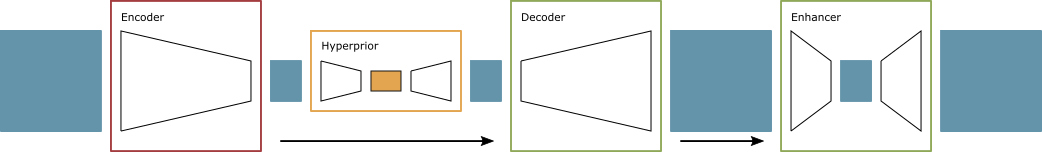
\includegraphics[width=\textwidth]{figure/general-enhance.png}
    \caption{The proposed model with all modules included.}
\end{figure}

Our entire compression framework is based on HiFiC \cite{mentzer_high_fidelity_2020}: we use the same structure of encoder and discriminator and similar decoder modules. Image can be represented using a convolutional features and we can train two neural networks to extract features from given image and reconstruct initial image from these features back. Such a network should have an encoder and a decoder. Encoder is trained to extract meaningful information form given image, which we call feature map or latents; Decoder is trained to reconstruct initial image given latents. We can train such system simply by penalizing $L1$ or $L2$ distance between given image and its reconstruction.

\begin{figure}[!ht]
    \centering
    \begin{tabular}{cc}
        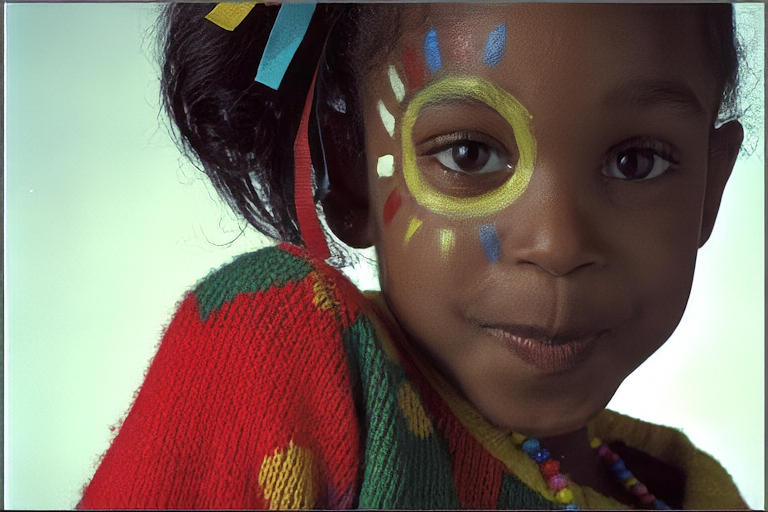
\includegraphics[width=.45\textwidth]{figure/kodim15_HiFiC_Lo.png} & 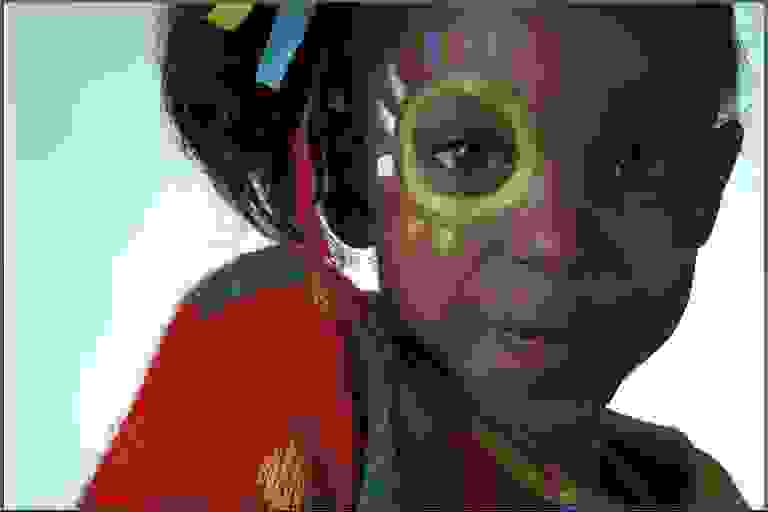
\includegraphics[width=.45\textwidth]{figure/kodim15_jpg_1x_0.166.jpg} \\
        a) Baseline model                                                  & b) JPEG
    \end{tabular}
    \caption{Neural image compression (HiFiC) comparison with JPEG (figure adapted from HiFiC results \cite{mentzer_high_fidelity_2020}).}
    \label{jpeg-hific-comparision}
\end{figure}

These intermediate convolutional features already take less disk space than raw initial image. However, we can compress these features using lossless coding algorithm. We are using arithmetic coding because of its huge capacity to compress sequences of numerical values.

It is not difficult to train an autoencoder to compress some information and decompress it back. So, we are using the same design as \cite{balle_variational_2018} to compress hidden features and obtain hyperlatents. Then they can be encoded by lossless compression algorithm.

After compressing image we need to be able to decompress these hyperlatent features back. Say we used lossless coding algorithm to decode hyperlatents, passed them to Hyperprior decoder and get latents. Then we feed these latents to fully convolutional decoder and apply deconvolution operation several times together with upscaling layers to make resulting image bigger. Finally we pass it through several super resolution layers to obtain an image with reduced blur artifacts, more sharp structure and, if needed, higher spacial resolution.

Such a system is complicated and since we need to train it efficiently, we consider using generative adversarial training pipeline to fit the model to data. Discriminator will be trained to till real and generated images apart, which will stabilize training same as in HiFiC \cite{mentzer_high_fidelity_2020}.

\section{JPEG compression}

As we described in the Introduction, JPEG is one of the most popular image compression pipelines. Understanding of this algorithm is essential for understanding a general image compression pipeline and the right place for each component in other algorithms. JPEG algorithm consists of several steps, which can be grouped into two main parts: compression and decompression.

\subsection{Compression algorithm}

\label{section:traditional-compression}

Chroma subsampling is a process of transformations from RGB format to YCbCr. YCbCr is a special format of storing image data not in Red, Green and Blue channels, but in Y, Cb and Cr channels. Y is the brightness channel of an image, Cb is the blue difference relative to the green color, Cr is the red difference relative to the green channel. After that it is already possible to reduce size by rescaling Cb and Cr channels by four. By doing so, the space is reduced by 1.5.

Compression of each channel is an performed in parallel. Image is partitioned into blocks 8x8 pixels. Each block is processed independently. Block values are centered at 0, so the values are in range (-127, 127). Then Discrete Cosine Transform (DCT) is being applied.

We can view an image as a combination of different frequencies. Pixel values can vary over given image, and we view this variation as a periodic function $f(x, y)$ where $x$ is horizontal coordinate and $y$ is a vertical one. There is a matrix of DCT coefficients, which consists of elements of different frequencies from low frequencies to high. High frequencies can be omitted to achieve better compression performance.

Mathematically, the DCT is one-to-one mapping for 64-point vectors between the image and the frequency domains. If the FDCT (Fast Discrete Cosine Transform) and IDCT could be computed with perfect accuracy and if the DCT coefficients were not quantized as in the following description, the original 64-point signal could be exactly recovered. In principle, the DCT introduces no loss to the source image samples; it merely transforms them to a domain in which they can be more efficiently encoded.

Each element of obtained matrix is a coefficient of corresponding frequency. Basically, the meaning of an element of this matrix is how much of this frequency is in given image. Then goes quantization, this step is lossy, and on this step elements of coefficients matrix are divided by so called standard JPEG quantization table. By the end of this procedure we have a matrix with coefficients. Relatively small coefficients can be omitted to react higher compression performance, since their frequencies contribution to image are tiny. Quantization table is specified as an input by application or user. Each element of quantization table is a number in range $(0; 255)$ which specifies the step size of the quantizer for its' corresponding DCT coefficient.

\begin{equation}
    \label{eq:00}
    F(u,v)=\dfrac{1}{4}C(u)C(v)[\sum_{x=0}^{7}\sum_{y=0}^{7}{f(x,y)*cos(\dfrac{(2x+1)u\pi}{16})*cos(\dfrac{(2x+1)v\pi}{16})}]
\end{equation}

\begin{equation}
    \label{eq:01}
    f(x,y)=\dfrac{1}{4}[\sum_{x=0}^{7}\sum_{y=0}^{7}{C(u)C(v)F(u,v)*cos(\dfrac{(2x+1)u\pi}{16})*cos(\dfrac{(2x+1)v\pi}{16})}]
\end{equation}

where:

\begin{equation}
    \label{eq:02}
    \begin{split}
        C(u), C(v) = \dfrac{1}{\sqrt{2}} \text{for } u,v=0 \\
        C(u), C(v) = 1 \text{otherwise}
    \end{split}
\end{equation}

Huffman coding is a type of entropy coding algorithms. This algorithm performs coding based on frequencies of each symbol in sequence. The goal is to encode most frequent symbols using less bits of information, since they appear in sequence more. Less frequent symbols are encoded using more bits of information since they appear in sequence less.

The result of Huffman coding is a Huffman tree \ref{huffman-tree}. To build this tree we need to follow the steps:

\begin{enumerate}
    \item Calculate frequencies of each symbol in sequence.
    \item Sort symbols in increasing order of frequencies.
    \item Make each unique symbol a leaf node (in other words, independent tree).
    \item Create an empty node and attach two leafs with smallest frequencies to this node as a children.
    \item Set value of this new node as a sum of it's children frequencies.
    \item Repeat steps 4-5 until thee is built.
    \item Each left edge must be labeled as $0$, each right edge must be labeled as $1$.
    \item Each symbol can be encoded using a path from the root node of a tree to this symbol.
\end{enumerate}

\begin{figure}[!ht]
    \centering
    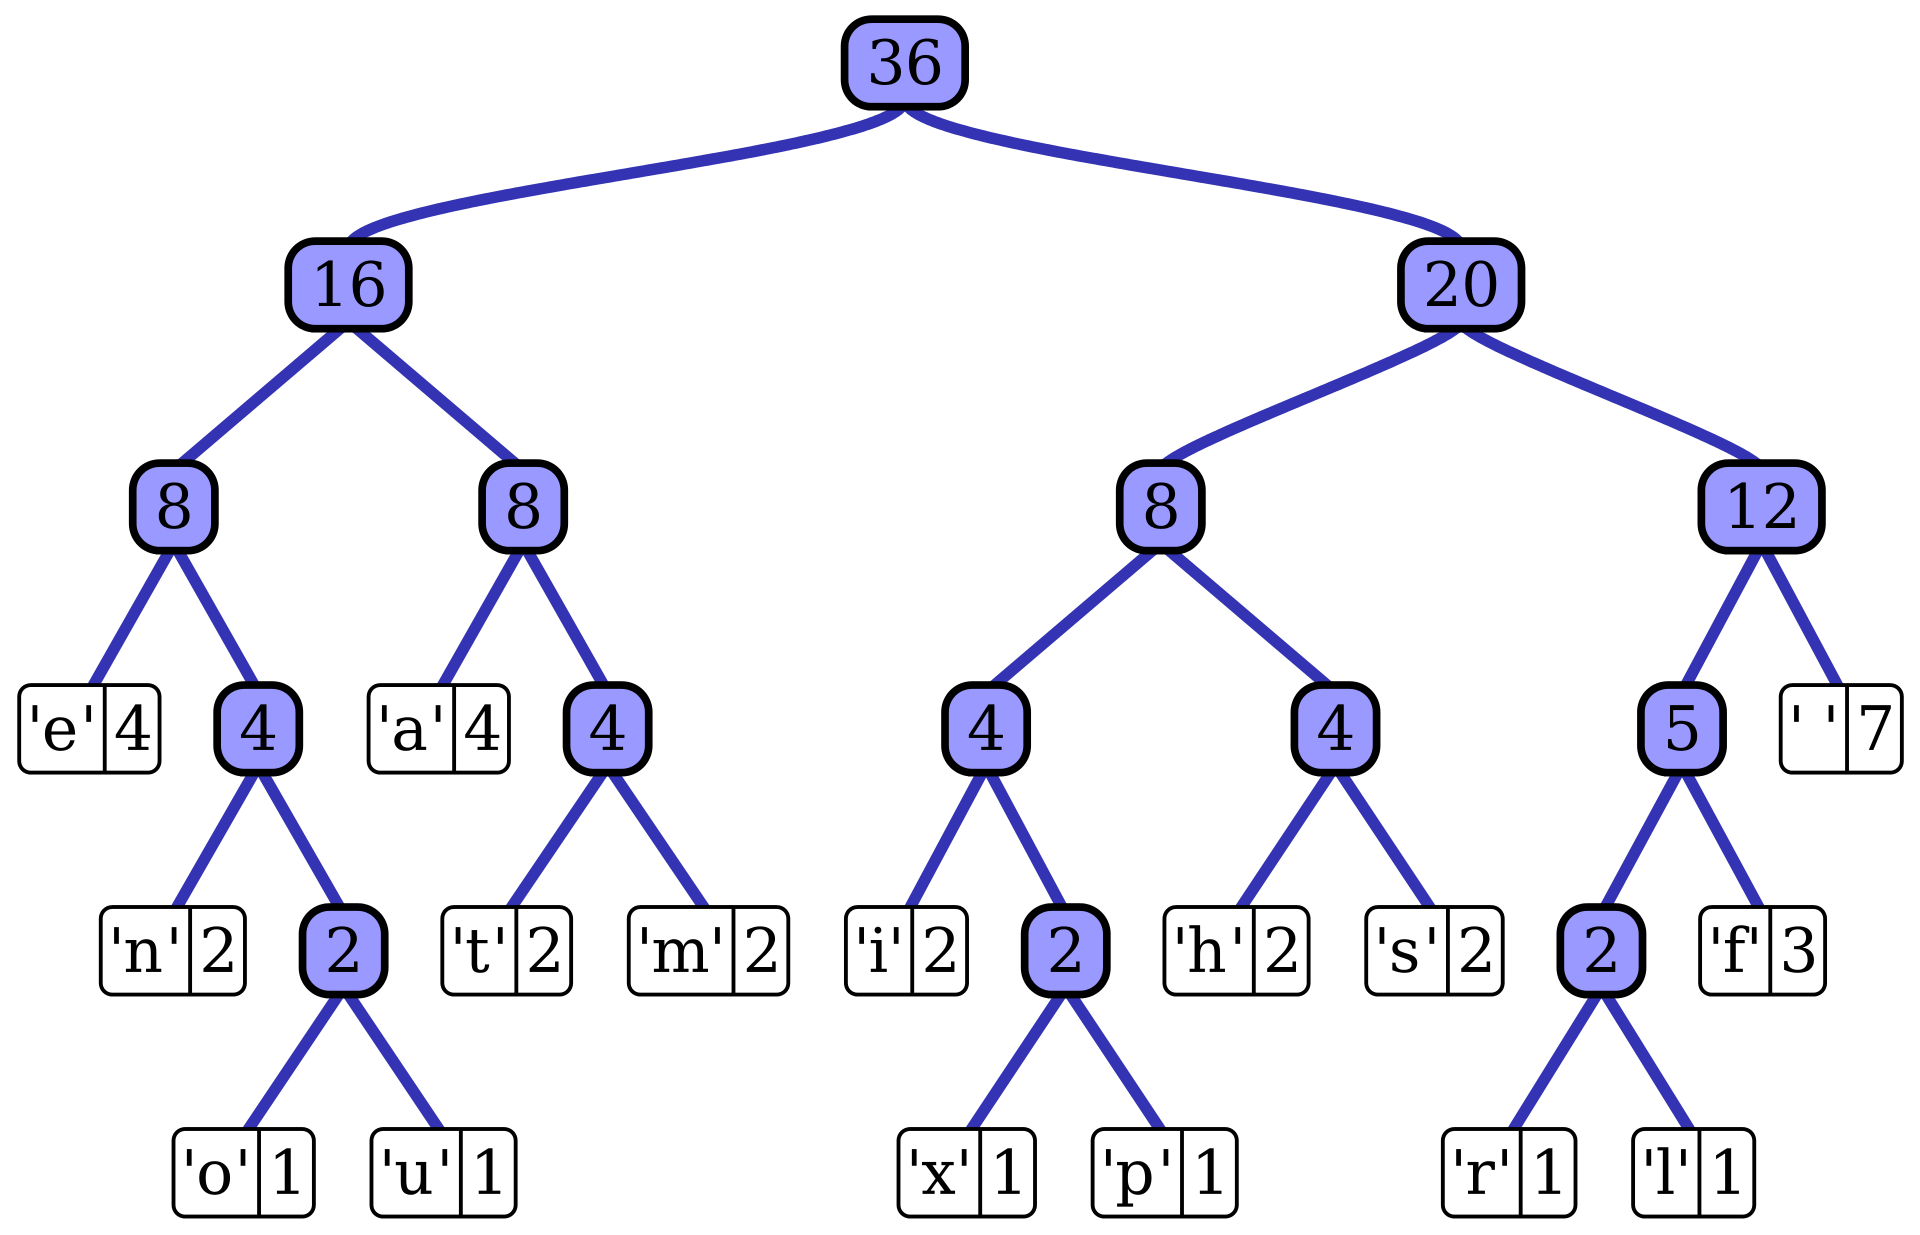
\includegraphics[width=\textwidth]{figure/Huffman_tree_2.svg.png}
    \caption{Huffman tree is a special type of binary tree. Each node of this tree can be described as a path from the root. This path consists of choices: left or right, which are encoded using ${0, 1}$}
    \label{huffman-tree}
\end{figure}

Huffman coding is performed on matrix obtained after DCT and quantization. this matrix is being reshaped to linear sequence (it is called Zig-Zag sequence, since the trajectory has a shape of zig-zag from top left corner up-down to the bottom-right corner).

\subsection{Decompression}

Decoding process consists of several steps, which are basically a reversed encoding steps.

\begin{enumerate}
    \item Decoding. Lossless.
    \item Dequantization. Lossy.
    \item Inverse Discrete Cosine Transform. Lossless.
    \item Transformation from YCbCr to RGB.
\end{enumerate}

To restore initial image first each block is passed through Huffman decoding algorithm. This step is lossless, so it just transforms a number with frequencies to a matrix obtained after DCT (during compression process).

For decoding Huffman codes it's required to take a code of the symbol and traverse through the Huffman tree. By the end of one traverse (in other words - reaching a leaf node), an original symbol is being obtained. So we can get a quantized coefficients matrix. To further continue decoding process dequantization is applied.

Dequantization is the inverse operation of quantization. Here it means that normalization is removed by multiplying by step size, which is specified in quantization table. To remind, this table is selected as an input information for the whole compression process before compression, and this is exactly same table as the one that was used during encoding process.

The next step is IDCT (Inverse Discrete Cosine Transform). IDCT takes the 64 DCT coefficients (which at that point have been quantized) and reconstructs a 64-point output image signal by summing the basis signals.

The last step of decompression is transformation from YCbCr representation to RGB. Ths transformation is a simple arithmetic which we omit here.

In JPEG format conversation from RGB to Y'CbCr and backwards are described in equation \ref{eq:chroma-forward} and equation \ref{eq:chroma-backward}, where Y, CB and CR are in the 8-bit range 0-255:

\begin{equation}
    \label{eq:chroma-forward}
    \begin{split}
        Y'=0+(0.299\cdot R'_{D})+(0.587\cdot G'_{D})+(0.114\cdot B'_{D}) \\
        C_{B}=128-(0.168736\cdot R'_{D})-(0.331264\cdot G'_{D})+(0.5\cdot B'_{D}) \\
        C_{R}=128+(0.5\cdot R'_{D})-(0.418688\cdot G'_{D})-(0.081312\cdot B'_{D})
    \end{split}
\end{equation}

Backwards:

\begin{equation}
    \label{eq:chroma-backward}
    \begin{split}
        R=Y+1.402\cdot (C_{R}-128) \\
        G=Y-0.34414\cdot (C_{B}-128)-0.71414\cdot (C_{R}-128) \\
        B=Y+1.772\cdot (C_{B}-128)
    \end{split}
\end{equation}

All these steps are reversible, which makes this algorithm stable and convenient to use in image compression. However, it has a couple of problems. One of these problems is an effective size of compressed image, as well as quality and consistency of compressed image. JPEG compression was introduced long time ago when computational power was not enough to perform calculations with high computational costs. At that time lightweight and rapid algorithm was needed to satisfy industry need. Now it is not necessary true. Modern compression approaches of course include a computationally expensive compression algorithms, such as neural compression.

\section{Autoencoder}

Autoencoder is a popular architecture for neural networks. It has been first introduced in \cite{Autoencoder_2006} and proven to be a powerful tool in dimensionality reduction tasks. Basically, autoencoders were introduced to solve a particular problem of dimensionality reduction. The goal of an original autoencoder is to reduce dimensionality of input tensor. PCA (principal component analysis) is a widely used method to perform a dimensionality reduction. PCA finds the directions of greatest variance over a dataset, and then represents each point in a dataset by its coordinates along these directions. These directions are called principal components and the number of principal components is significantly less than number of components of original data point.

PCA uses a statistical approach to fit data. More precise, PCA is based on Eigen-decomposition, where we find a matrix of eigenvectors and eigenvalues of the covariance matrix and take $N$ biggest eigenvalues and $N$ corresponding eigenvectors. These are called principal components.

Similarly to PCA, autoencoder reduces dimensionality of an original data point, but the core principle of autoencoder is different from PCA. Instead of having a fixed algorithm to reduce dimensionality, autoencoders employs a power of neural networks. Autoencoder has two networks: encoder and decoder. Encoder is a network that embeds an original data into space with much smaller dimensions by sequentially passing original data through convolutional layers. These layers reduce dimensions of data, keeping however the most significant information. After the encoder, reduced features go through decoder, which increases dimensionality of data to its' original shape.

\begin{figure}[!ht]
    \centering
    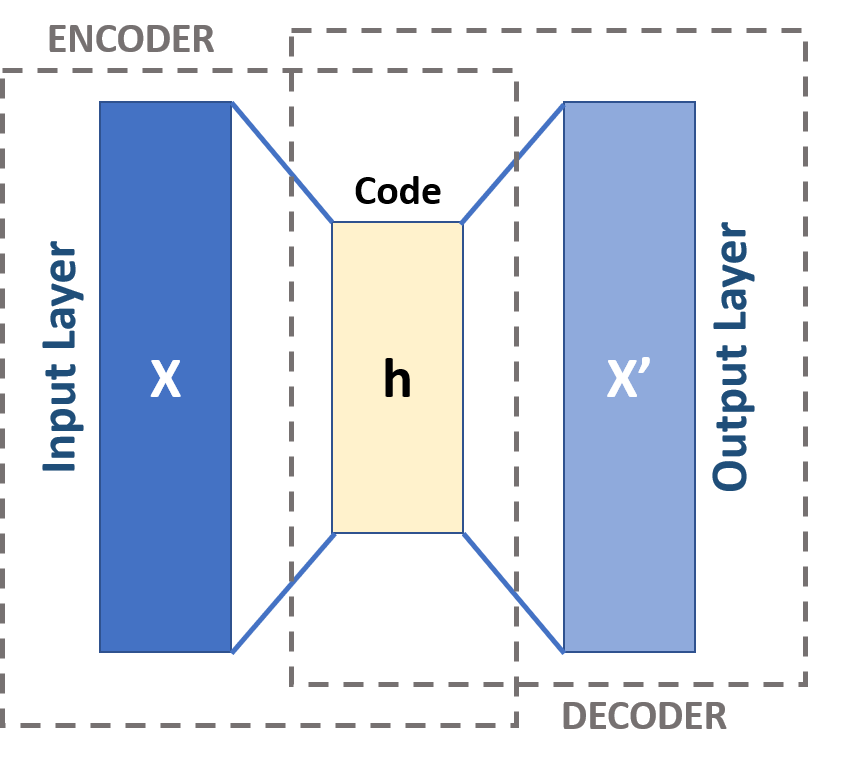
\includegraphics[width=\textwidth]{figure/Autoencoder_schema.png}
    \caption{Autoencoder schema.}
    \label{autoencoder-schema}
\end{figure}

Autoencoder architecture is a very popular choice. Recent years a number of publications that use an autoencoder model one way or another, which is shown in figure \ref{autoencoder-popularity-dynamics}.

\begin{figure}[!ht]
    \centering
    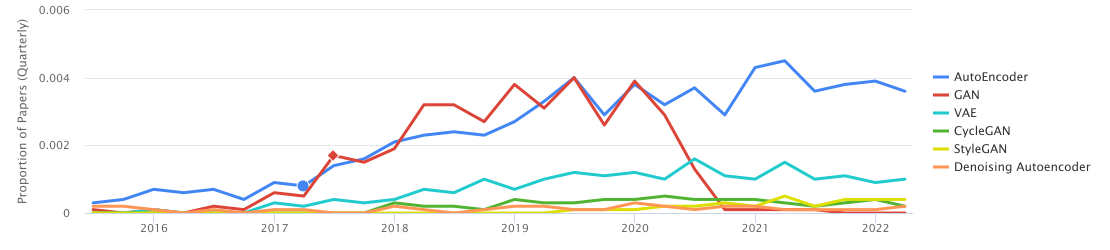
\includegraphics[width=\textwidth]{figure/autoencoder-popularity-over-time.png}
    \caption{Autoencoder architecture popularity over time compared to other popular neural network architectures (data from Papers With Code \cite{autoencoder_papers})}
    \label{autoencoder-popularity-dynamics}
\end{figure}

Autoencoder is trained in supervised manner: feed data, pass it through encoder and decoder, calculate difference between original image in the output, then back propagate. After sufficient amount of iterations autoencoder finds its' local minimum. At this moment we need to stop training process, store weights and fix them.

Autoencoders have many applications (figure \ref{autoencoder-popularity-stats}) in compression, denoising, debluring, upscaling etc. The conceptual idea in all these applications is that hidden representation is a compressed version of input data, then original data is restored by generator. The loss here is significant since this is actually the criteria of autoencoder performance and for different tasks the criteria is formulated differently.

\begin{figure}[!ht]
    \centering
    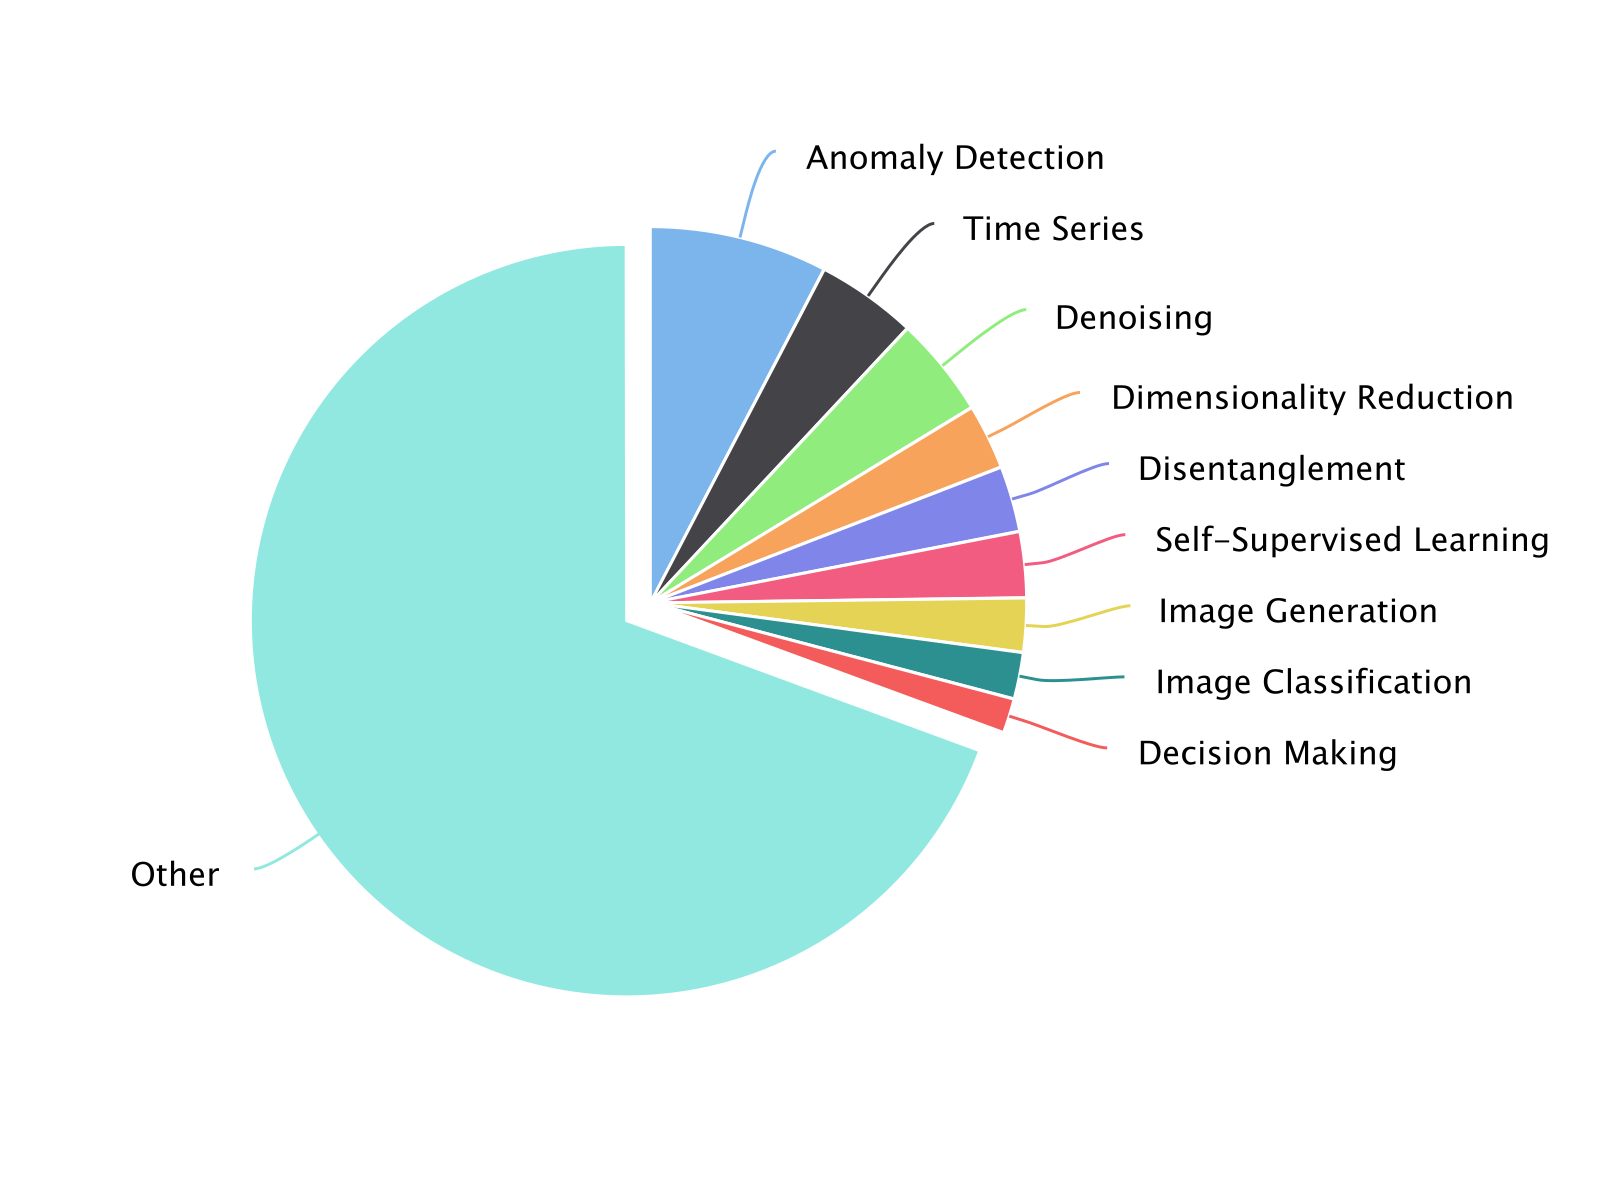
\includegraphics[width=\textwidth]{figure/autoencoder-popularity-stats.png}
    \caption{Autoencoder architecture usage statistics by paper' subject (data from Papers With Code website \cite{autoencoder_papers})}
    \label{autoencoder-popularity-stats}
\end{figure}

We use fully convolutional neural networks (FCN) in the encoder from the figure \ref{encoder}. FCNs are a family of convolutional neural networks which does not use pooling layers or bilinear interpolation or any other layer that can cause an information loss. Layers like pooling layer only propagate one value though itself. It causes a situation when we cannot determine or learn any information about input to this layer knowing it's output.

\subsection{Autoencoder probability model}

Autoencoder is a sequential application of the encoder function $z=g(x)$ and decoder $x^*=f(z)$, where $x$ is the input vector and $z$ is the latent representation. In some subset of the input data (usually close to the training set) $x^*=x+n=f(g(x))$, where $n$ is the residual. We will take the residual as a Gaussian noise (its' parameters can be estimated after training the autoencoder). As a result, a number of fairly strong assumptions are made:

\begin{itemize}
    \item The residual is Gaussian noise
    \item The autoencoder is already "trained" and works
\end{itemize}

But, importantly, there will be almost no restrictions imposed on the autoencoder itself.

Then we can get a qualitative estimate of the probability density $p(x)$, based on which we can draw several very important conclusions.

The distribution density for $x\in X$ and $z\in Z$ are related as follows:

\begin{equation}
    \label{eq:autoencoder-density}
    p(x) = \int_{z} p(x|z)p(z)dz
\end{equation}

We need to determine the relation $p(x)$ and $p(z)$. For some autoencoders, $p(z)$ is set at the stage of their training, for others it is easier to get $p(z)$ with the smaller dimensionality of $Z$.

The noise distribution density $n$ is known, so:

\begin{equation}
    \label{eq:autoencoder-noise-density}
    p(n)=const\times exp( -\frac{(x-f(z))^T (x-f(z))}{2\sigma^2} )=p(x|z)
\end{equation}

Where $(x-f(z))^T (x-f(z))$ is the distance between $x$ and its projection $x^*$. At some point $z^*$ this distance will reach its minimum. At this point, the partial derivatives of the exponent argument in formula \ref{eq:autoencoder-noise-density} by $z_i$ ($Z$ axes) are zero:

\begin{equation}
    \label{eq:autoencoder-derivatives}
    0 = \frac{\partial f(z^*)}{\partial z_i}^T(x-f(z^*))+(x-f(z^*))^T\frac{\partial f(z^*)}{\partial z_i}
\end{equation}

Here $\frac{\partial f(z^*)}{\partial z_i}^T(x-f(z^*))$ is a scalar, then:

\begin{equation}
    \label{eq:autoencoder-derivatives-1}
    0 = \frac{\partial f(z^*)}{\partial z_i}^T(x-f(z^*))
\end{equation}

Selecting a point $z^*$, where the distance is $(x-f(z))^T (x-f(z))$ is minimal, happens during the autoencoder optimization process. During training, it is the quadratic residual that is minimized (usually):

\begin{equation}
    \label{eq:autoencoder-minimized}
    \min\limits_{\theta, \forall x\in X train} L2_{norm}({x-f_\theta(g_\theta(x))})
\end{equation}

Where $\theta$ is the weights of the autoencoder. I.e. after training, $g(x)$ tends to $z^*$.

We can also decompose $f(z)$ into a Taylor series (up to the first term) around $z^*$:

\begin{equation}
    \label{eq:autoencoder-taylor}
    f(z)=f(z^*)+\nabla f(z^*)(z-z^*)+o((z-z^*))
\end{equation}

So, now equation \ref{eq:autoencoder-noise-density} will become:

\begin{equation}
    \label{eq:autoencoder-}
    \begin{split}
        p(x|z) \approx const\times exp( -\frac{((x-f(z^*))-\nabla f(z^*)(z-z^*))^T ((x-f(z^*))-\nabla f(z^*)(z-z^*))}{2\sigma^2} )=\\
        const\times exp(-\frac{(x-f(z^*))^T(x-f(z^*))}{2\sigma^2})exp(-\frac{(\nabla f(z^*)(z-z^*))^T(\nabla f(z^*)(z-z^*))}{2\sigma^2}) \times \\
        \times exp(-\frac{( \nabla f(z^*)^T(x-f(z^*))+(x-f(z^*))^T\nabla f(z^*))(z-z^*)}{2\sigma^2})
    \end{split}
\end{equation}

Note that the last multiplier is equal to 1 due to expression \ref{eq:autoencoder-derivatives-1}. The first multiplier can be taken as the sign of the integral (it does not contain $z$) in equation \ref{eq:autoencoder-density}. And also assume that $p(z)$ is a fairly smooth function and does not change much in the neighborhood of $z^*$, i.e. replace $p(z)$ by $p(z^*)$.

After all assumptions, integral from the equation \ref{eq:autoencoder-density} has an estimate:

\begin{equation}
    \label{eq:autoencoder-probability-estimation}
    \begin{split}
        p(x) = const\times p(z^*)exp(-\frac{(x-f(z^*))^T(x-f(z^*))}{2\sigma^2}) \int_{z}exp(-(z-z^*)^TW(x)^TW(x)(z-z^*)) dz, z^*=\\
        g(x)
    \end{split}
\end{equation}

Where $W(x)=\frac{\nabla f(z^*)}{\sigma}, z^* = g(x)$

The last integral is the n-dimensional Euler-Poisson integral:

\begin{equation}
    \label{eq:autoencoder-euler-poisson}
    \int_{z}exp(-\frac{(z-z^*)^TW(x)^TW(x)(z-z^*)}{2}) dz=\sqrt{\frac{1}{det(W(x)^TW(x)/2\pi)}}
\end{equation}

As a result, we got the final estimate of $p(x)$:

\begin{equation}
    \label{eq:autoencoder-density-final}
    p(x) = const\times exp(-\frac{(x-f(z^*))^T(x-f(z^*))}{2\sigma^2})p(z^*)\sqrt{\frac{1}{det(W(x)^TW(x)/2\pi)}}, z^*=g(x)
\end{equation}

All this math was needed to show that $p(x)$ depends on three factors:

\begin{itemize}
    \item The distances between the input vector and its reconstruction, the worse the reconstruction, the smaller the $p(x)$
    \item Probability density $p(z^*)$ at the point $z^*=g(x)$
    \item Normalization of the function $p(z)$ at the point $z^*$, which is calculated for the autoencoder from partial derivatives of the function $f$
\end{itemize}

And also from the normalization constant, which will subsequently be responsible for the a priori probability of choosing an autoencoder to describe the input data.

Despite all the assumptions, the result turned out to be very meaningful and useful from the calculations.

\subsection{Encoder}

Let us consider a pooling layer as an example to make our concern clear. Pooling layer takes a patch from an image (or from a feature map) and aggregates all those values into single output value. Pooling layers usually make use of aggregation functions such as \textit{max}, \textit{min}, \textit{avg} etc. Those functions are permutation invariant and they do not have an inverse function, which means we cannot reverse them. Even in theory it is impossible to get an inverse functions for pooling layers kernels, since pooling operation causes information loss.

\begin{figure}[!ht]
    \centering
    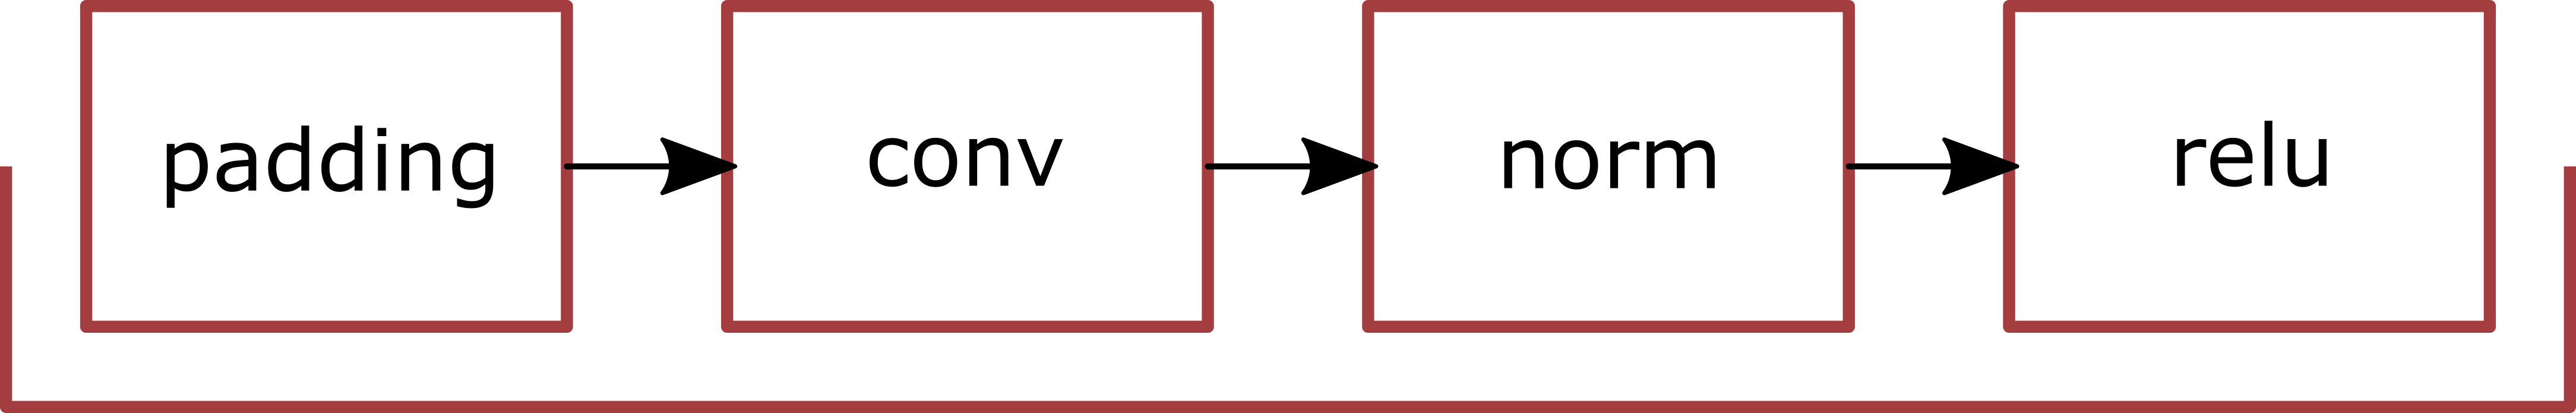
\includegraphics[width=\textwidth]{figure/encoder.png}
    \caption{Convolutional block of the encoder. We stack 6 such blocks to obtain encoder.}
    \label{encoder}
\end{figure}

This is the reason pooling layers are not used or seldom used in neural image compression and other neural compression models. As a fairly good alternative for traditional convolutional networks with pooling layers we use FCNs mentioned the the previous subsection.

\subsection{Decoder}

After a motivation for using FCNs in our encoder, let us take a look on the decoder in the figure \ref{decoder}. And the logic here is absolutely same: To restore an image given hidden feature map we need to learn an inverse function, which can be only obtained by reverse of encoder. In practice it means that we need both encoder and decoder to be FCNs (figure \ref{autoencoder}). It will make the entire pipeline less lossy and make an intermediate features more interpretable, since using only convolutional layers helps to achieve a certain consistency in mapping features from input of one layer to its output.

\begin{figure}[!ht]
    \centering
    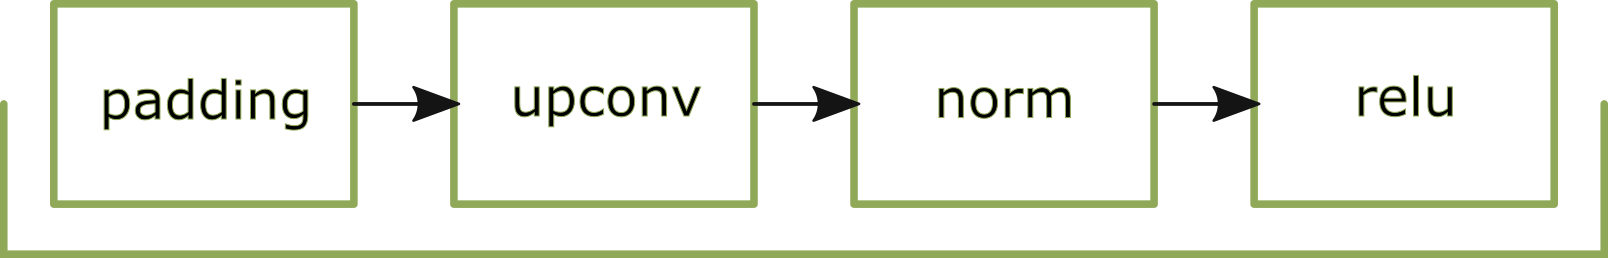
\includegraphics[width=\textwidth]{figure/generator.png}
    \caption{Upconvolutional block (top) and residual block (bottom) of the decoder. We use a combination of these two blocks: We stack 8 residual blocks with 6 upconvolutional blocks on top.}
    \label{decoder}
\end{figure}

We are also using normalization layers in encoder and decoder to make a network more stable. And each convolutional and normalization layer has a residual connection.

\begin{figure}[!ht]
    \centering
    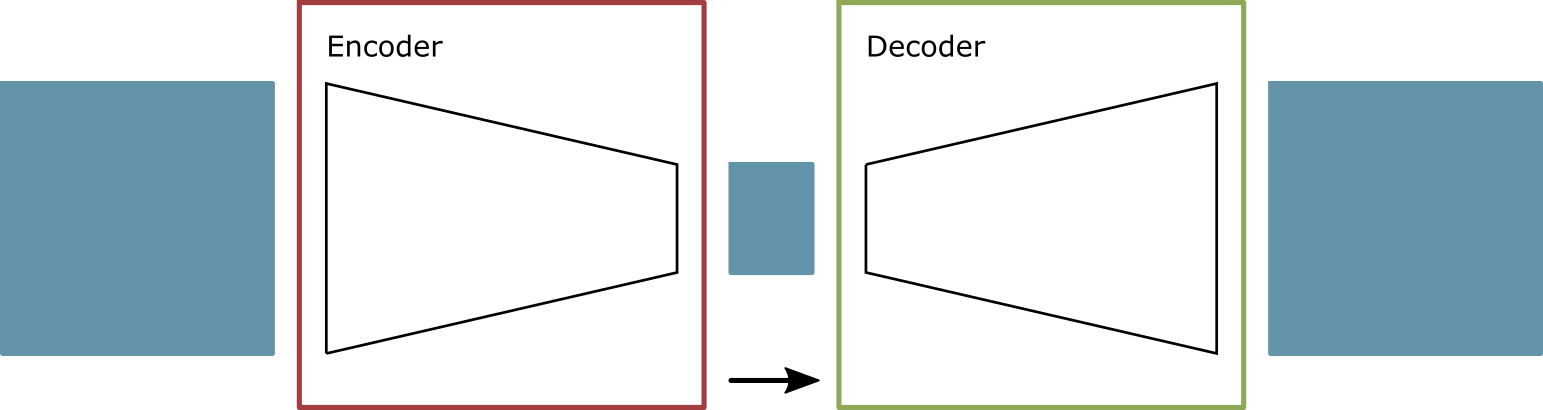
\includegraphics[width=\textwidth]{figure/general-autoencoder.png}
    \caption{Simple autoencoder architecture, which is used in this work. Encoder and decoder are FCNs. Data flow is highlighted to blue. Features in the middle have more channels but less height and width than original image, and this hidden representation takes less space than initial image.}
    \label{autoencoder}
\end{figure}

\subsection{Autoencoder training}

We can train this autoencoder by minimizing L1 in the equation \ref{eq:1} and L2 in the equation \ref{eq:2} distance losses. This is a general pipeline for training autoencoder for image compression. Usually other terms are added to the final loss. But even using this simple pipelines we can still reach a reasonable results (on the figure \ref{autoencoder-result}).

\begin{figure}[!ht]
    \centering
    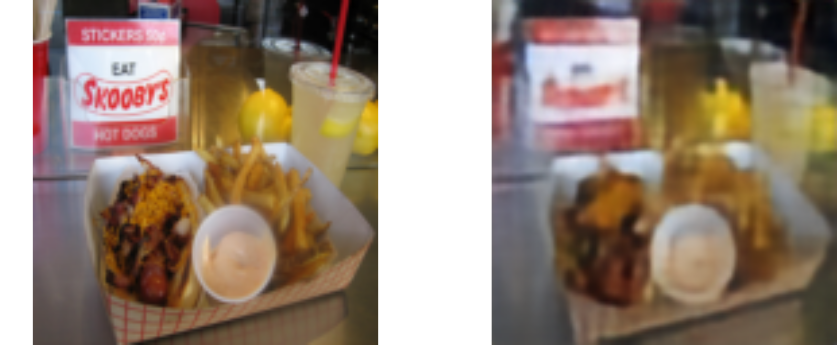
\includegraphics[width=\textwidth]{figure/autoencoder-result.png}
    \caption{Results obtained by training simple autoencoder. (left) Original image, (right) Image obtained after encoding and decoding  using FCN encoder and decoder.}
    \label{autoencoder-result}
\end{figure}

L2 distance loss can be obtained using formula below \ref{eq:2}

\begin{equation}
    \label{eq:2}
    L2=\sum (\hat{I}-I)^2
\end{equation}

\begin{equation}
    \label{eq:1}
    L1=\sum \hat{I}-I
\end{equation}

Having hidden features (or latents), we can then compress them using one of lossless algorithms such as arithmetic coding or even Huffman coding algorithms. Since we have numerical values here, arithmetic coding is more preferable.

It is possible to use another autoencoder to encode latents obtained from the encoder into hyperlatents, that will have even smaller dimensionality, and apply arithmetic coding to these hyperlatents. We are using a Hyperprior module, which was described in \cite{balle_variational_2018}

\begin{figure}[!ht]
    \centering
    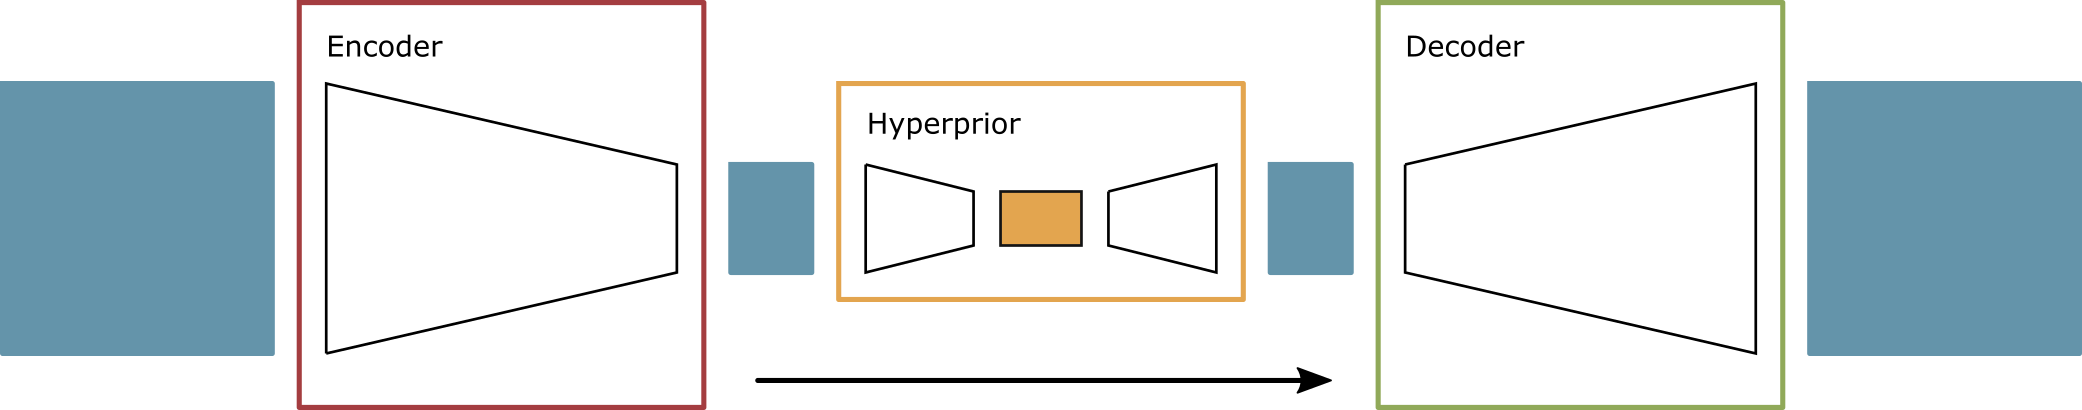
\includegraphics[width=\textwidth]{figure/general.png}
    \caption{Compression general pipeline. Encoder is used to obtain latents, then another encoder is used to obtain hyperlatents. Yellow block is quantization and arithmetic coding block. Then hyperlatents are decoded to latents and the last step is to pass it though Decoder to obtain reconstructed image.}
    \label{whole-system-geneal-pipeline}
\end{figure}

\section{Coding}

The last step of compression is coding. Coding is lossless, and basically it is an independent algorithm. Usually arithmetic coding or Huffman coding are used.

\subsection{Huffman coding}

We have briefly described Huffman coding algorithm in \nameref{section:traditional-compression}. Now let us trace the Huffman algorithm step by step.

The method is based on the binary trees data structure. In it, the node can be either terminal or internal. Initially, all nodes are considered leaves (terminal), which represent the symbol itself and its weight (that is, the frequency of occurrence in the sequence). The internal nodes contain the weight of the symbol and refer to two successor nodes. By general convention, bit $0$ represents following the left branch, and $1$ represents following the right. There are $N$ leaves and $N-1$ internal nodes in a complete tree. It is recommended that when constructing the Huffman tree, unused characters are discarded to obtain codes of optimal length.

We will use a priority queue to build a Huffman tree, where the node with the lowest frequency will be assigned the highest priority. The construction steps are described below:

\begin{enumerate}
    \item Create a leaf node for each symbol and add them to the priority queue.
    \item While there is more than one sheet in the queue, we do the following:
          \begin{enumerate}
              \item Remove the two nodes with the highest priority (with the lowest frequency) from the queue;
              \item Create a new internal node where these two nodes will be children, and the frequency of occurrence will be equal to the sum of the frequencies of these two nodes.
              \item Add a new node to the priority queue.
          \end{enumerate}
    \item The only remaining node will be the root node, and the tree construction will end there.
\end{enumerate}

Let us consider some text that consists only of the characters "a", "b", "c", "d" and "e", and the frequencies of their occurrence are 15, 7, 6, 6 and 5, respectively. Below are illustrations that reflect the steps of the algorithm.

On the first state we have a set of leaf nodes with attached frequencies and characters they encode (figure \ref{huffman-0}).

\begin{figure}[!ht]
    \centering
    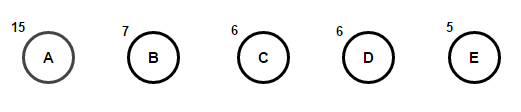
\includegraphics[width=0.7\textwidth]{figure/huffman-0.png}
    \caption{Huffman tree on the beginning of the algorithm}
    \label{huffman-0}
\end{figure}

We take two less frequent symbols from the queue and attach them to one newly created internal node and the frequency of this node is the sum of its' children frequencies (figure \ref{huffman-1}). The newly created node is added to priority queue.

\begin{figure}[!ht]
    \centering
    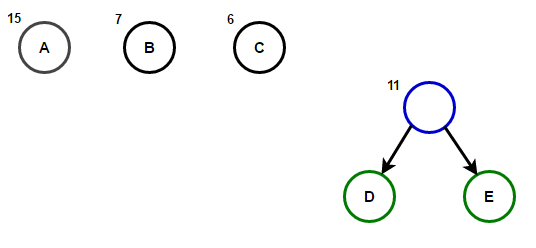
\includegraphics[width=0.7\textwidth]{figure/huffman-1.png}
    \caption{Huffman tree after the first step.}
    \label{huffman-1}
\end{figure}

On the next step we take next two most frequent nodes from the queue and create a new node, obtain frequency by summing up its' children. The newly created node is added to priority queue.

\begin{figure}[!ht]
    \centering
    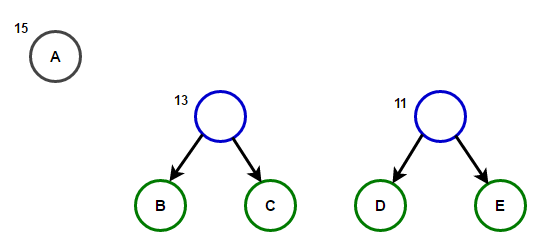
\includegraphics[width=0.7\textwidth]{figure/huffman-2.png}
    \caption{Huffman tree after the second step.}
    \label{huffman-2}
\end{figure}

Continue by taking two less frequent nodes from the queue and attach them to newly created node, obtain frequency for it. The newly created node is added to priority queue.

\begin{figure}[!ht]
    \centering
    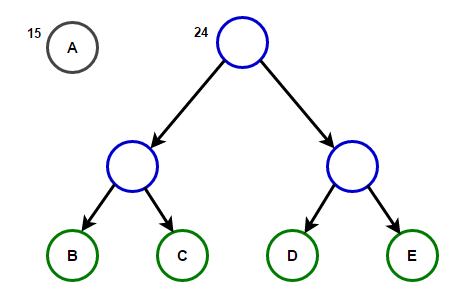
\includegraphics[width=0.7\textwidth]{figure/huffman-3.png}
    \caption{Huffman tree after the third step.}
    \label{huffman-3}
\end{figure}

The last node is taken from the queue and attached to newly created tree, the root node frequency is sum of all the frequencies of its' children.

\begin{figure}[!ht]
    \centering
    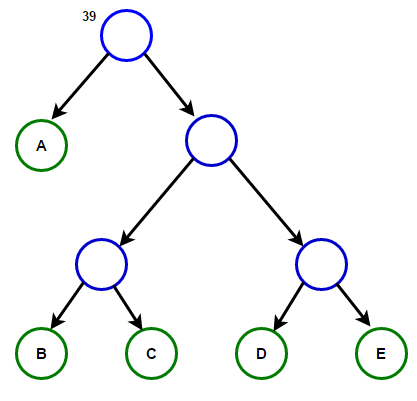
\includegraphics[width=0.7\textwidth]{figure/huffman-4.png}
    \caption{Huffman tree after the fourth step.}
    \label{huffman-4}
\end{figure}

Priority queue is empty now an it means that the tree building is completed. every left edge is labeled as $0$ and every right edge is labeled as $1$. Each symbols' code is obtained by traversing this tree from root to the symbol. The path is determined by labels of the edge we pas through. For example, the code for symbol "b" is $100$.

\begin{figure}[!ht]
    \centering
    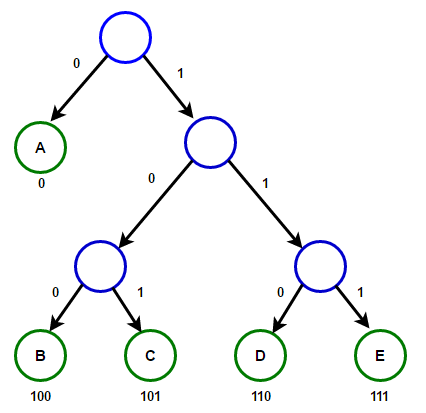
\includegraphics[width=0.7\textwidth]{figure/huffman-5.png}
    \caption{Huffman tree after the fifth step.}
    \label{huffman-5}
\end{figure}

Since efficient priority queue data structures require $O(log(N))$ time to insert, and there are $2N-1$ nodes in a complete binary tree with $N$ leaves, and the Huffman tree is a complete binary tree, the algorithm works in $O(N log(N))$ time, where $N$ is the number of characters.

\subsection{Arithmetic coding}

Arithmetic coding is a form of entropy coding (figure \ref{arithmetic_coding}). It is lossless, which means that after compression and decompression no information is lost. It is used to compress numeric sequencies, which makes it perfect for the task of image compression since after quantization process we have exactly what is required - a list of integers. According to Shannon's source coding theorem an optimal representation converges to $log_2P$ bits per symbol for a symbol with frequency $P$.

The first step of arithmetic coding is building of probability information from source sequence. After knowing all the probabilities we need to place them according to their probabilities. Then the range of the first symbol is set to be a next range. Then the process is repeated $N$ times, where $N$ is a length of sequence. By the end of this process we have a single segment in the global range (on the figure \ref{arithmetic_coding} it is the range from $0.534$ to $0.54$). Then we just pick a number from this range. This number is a compressed sequence.

\begin{figure}[!ht]
    \centering
    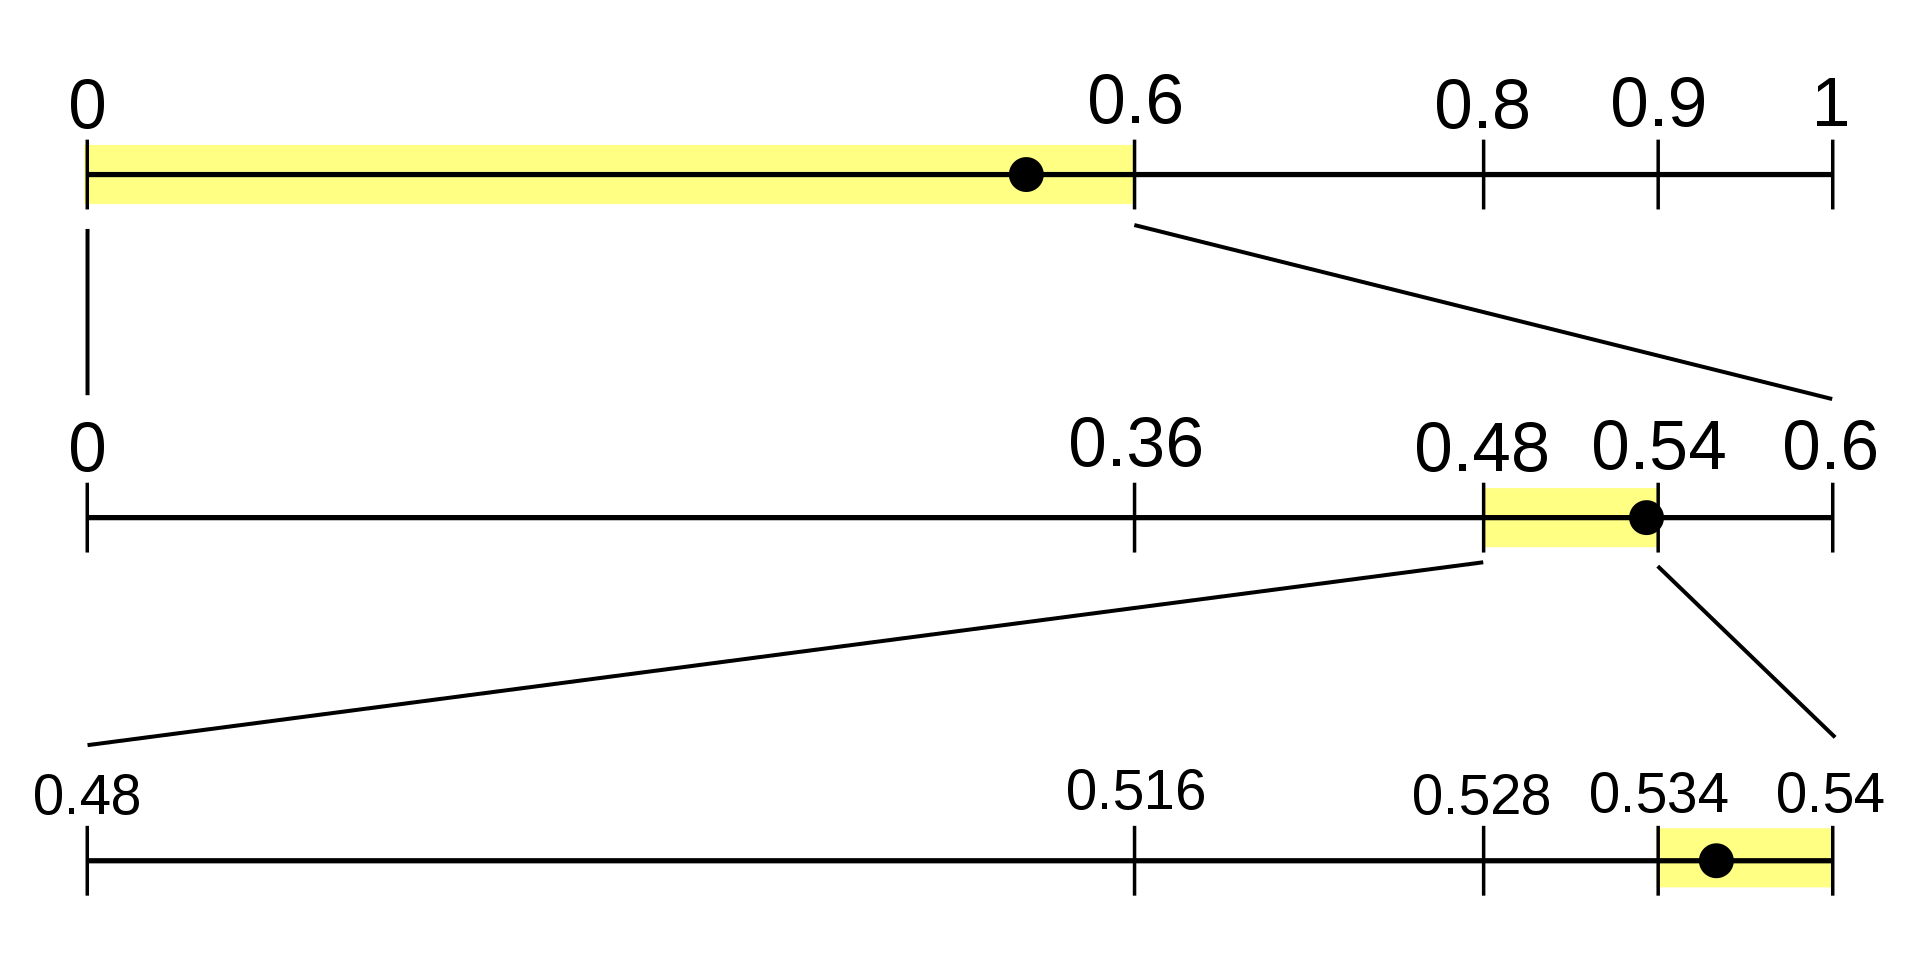
\includegraphics[width=\textwidth]{figure/Arithmetic_encoding.svg.png}
    \caption{Arithmetic coding for a sequence with length 3. Each horizontal segment represents a position in sequence, and parts of these segments correspond to probabilities or frequencies of the symbols they are related to.}
    \label{arithmetic_coding}
\end{figure}

Compressed sequence is stored as a single number. It's also required to remember probabilities since they are used in decompression process.

\section{Generative adversarial network}

Generative modeling involves the approximation of non-computable a posteriori distributions. Because of this, most effective methods developed for training discriminative models do not work with generative models. The methods existing in the past to solve this problem are computationally difficult and are mainly based on the use of the Markov Chain Monte Carlo, which is poorly scalable. Therefore, to train generative models, a method based on scalable techniques such as Stochastic Gradient Descent (SGD) and backpropagation was needed. One of these methods is Generative Adversarial Networks (GAN). GANs were first proposed in 2014. At a high level, this model can be described as two submodels that compete with each other, and one of these models (the generator) is trying to learn to deceive the second one (the discriminator) in some sense. To do this, the generator generates random objects, and the discriminator tries to distinguish these generated objects from real objects from the training sample. During the learning process, the generator generates objects that are more and more similar to the sample, and it becomes increasingly difficult for the discriminator to distinguish them from the real ones. Thus, the generator turns into a generative model that generates objects from a certain complex distribution, for example, from the distribution of photographs of human faces.

Generative adversarial networks (GANs) show a great performance in training generative models. For GANs training pipeline is slightly different from traditional deep learning pipeline. In \cite{Goodfellow_Pouget-Abadie_Mirza_Xu_Warde-Farley_Ozair_Courville_Bengio_2014} they introduced a neural network training pipeline with two networks: generator and discriminator. Generators objective is to produce a good enough synthetic data. Discriminators objective is to find out, whether given sample synthetic or real. So, trained generator network can be used then to solve a problem.

\subsection{Basics}

Usually when we deal with some operation that modifies an original image, but that also must keep a consistency from image to image and keep some features that are significant for the model performance, it is reasonable to use GAN pipeline for training. Such features can be style features for example. In case of image compression it's more simple: the discriminator network is penalized to till apart images that are original and images that were passed through the model (compressed and decompressed).

Since our model is a neural network and compression power of the network is due to its' convolutional neural network nature, we can use GAN training pipeline to further improve model performance.

GAN objective is formulated in \cite{Goodfellow_Pouget-Abadie_Mirza_Xu_Warde-Farley_Ozair_Courville_Bengio_2014}. Main GAN loss is described in the equation \ref{eq:gan-loss} it consists of two terms: generator and discriminator losses.

\begin{equation}
    \label{eq:gan-loss}
    min_G max_D V(D, G) = E_{x~p_{data}(x)} [log D(x)] + E_{z~p_z(z)} [log(1 - D(G(z)))]
\end{equation}

During training GAN learns a generator distribution $p_g$ over data $x$, $p_z(z)$ is a prior on input noise variables. $G(z, \Theta_g)$ is a mapping to data space, where $G$ is a differentiable function (neural network with parameters $\Theta_g$). There also is a second network $D(x, \Theta_d)$ that outputs a single scalar. $D(x)$ represents the probability that input $x$ came from the data rather than $p_g$. $D$ is trained to maximize the probability of assigning the correct label to both training examples and samples from $G$. $G$ simultaneously trained to minimize $log(1 − D(G(z)))$. The objective is to maximize discriminator loss and minimize generator loss.

\subsection{Model}

To begin with, we will introduce the necessary terminology. By $X$ we denote a certain space of objects. For example, images of $64*64*3$ pixel. On some probabilistic image space $\Omega$ a vector random variable $x:\Omega \rightarrow X$ is given with a probability distribution with density $p(x)$ such that a subset of the space $X$ on which $p(x)$ takes non—zero values is, for example, photographs of human faces. We are given a random sample of photos for $\{x_i, i \in [1, N], x_i \sim p(x)\}$. Additionally, we define the auxiliary space $Z=R^n$ and the random variable $z:\Phi \rightarrow Z$ with a probability distribution having the density $q(z)$. $D:X \rightarrow (0, 1)$ is a discriminator function. This function takes an image object as input (in our example, an image of the appropriate size) and returns the probability that the input image is a photograph of a human face. $G:Z \rightarrow X$ — generator function. It takes the value $z \in Z$ and outputs an object of the space $X$, that is, in our case, a picture.

Suppose we already have an ideal discriminator $D$. For any $x$ sample, it outputs the true probability that this example belongs to a given subset of $X$ from which ${x_i}$ sample was obtained. Reformulating the task of deceiving the discriminator in probabilistic language, we get that it is necessary to maximize the probability given by the ideal discriminator on the generated examples. Thus, the optimal generator is such that:

\begin{equation}
    \label{eq:gan-00}
    G^* = argmax_G E_{z~q(x)}D_k(G(z))
\end{equation}

Since $log(x)$ is a monotonically increasing function and does not change the position of the extremums of the argument, this formula can be rewritten in the form of equation \ref{eq:gan-0}.

\begin{equation}
    \label{eq:gan-0}
    G^* = argmax_G E_{z~q(x)} log D_k(G(z))
\end{equation}

In reality, there is usually no ideal discriminator and it must be found. Since the task of the discriminator is to provide a signal for training the generator, instead of an ideal discriminator, it is enough to take a discriminator that ideally separates the real examples from those generated by the current generator, i.e. ideal only on a subset of $X$ from which the examples are generated by the current generator. This task can be reformulated as a search for such a function $D$ that maximizes the probability of correctly classifying examples as real or generated. This is called a binary classification problem, and in this case we have an infinite training sample: a finite number of real examples and a potentially infinite number of generated examples. Each example has a label: it is real or generated. The first article described the solution of the classification problem using the maximum likelihood method.

So, our set $S=\{(x, 1), x~p(x)\} \cup \{G(z), 0\, z \sim q(z)\}$. Let's determine the density of distribution $f(\xi|\nu=1) = D(\xi), f(\xi|\nu=0)=1-D(\xi)$, then $f(\xi|\nu)$ is a reformulation of $D$, which gives out the probability of the class $1$ (this example) in the form of a distribution on the classes $\{0, 1\}$. Since $D(\xi) \in (0, 1)$, this definition sets the correct probability density. Then the optimal discriminator can be found as:

\begin{equation}
    \label{eq:gan-1}
    D^* = f^*(\xi|\nu) = argmax_f f(\xi_1, \dots | \nu_1, \dots) = argmax_f \prod_i f(\xi_i|\nu_i)
\end{equation}

Group the multipliers for $\nu_i=0$ and $\nu_i=1$:

\begin{equation}
    \label{eq:gan-2}
    \begin{split}
        D^* = argmax_f \prod_{i, \nu=1} f(\xi_i|\nu_i=1) \prod_{i, \nu=0} f(\xi_i|\nu_i=0) = \\
        = argmax_D \prod_{x_i~p(x)} D(x_i) \prod_{z_i~q(z)} (1 - D(G(z_i))) = \\
        = argmax_D \sum_{x_i~p(x)} log D(x_i) + \sum_{z_i~q(z)} log (1 - D(G(z_i)))
    \end{split}
\end{equation}

And when the sample number tends to infinity, we get:

\begin{equation}
    \label{eq:gan-3}
    D^* = argmax_D E_{x_i~p(x)} log D(x_i) + E_{z_i~q(z)} log (q - D(G(z_i)))
\end{equation}

In total, we get the following iterative process:

\begin{enumerate}
    \item Setting an arbitrary initial $G_0(z)$.
    \item The $k$ iteration begins, $k=1 \dots K$.
    \item We are looking for an optimal discriminator for the current generator: \\
          $D_k = argmax_D E_{x_i~p(x)} log D(x_i) + E_{z_i~q(z)} log(1 - D(G_{k-1}(z_i)))$
    \item Improving the generator using the optimal discriminator:

    \item $G_k = argmax_G E_{z~q(x)} log(D_k(G(z)))$. It is important to be in the vicinity of the current generator. If we move away from the current generator, the discriminator will cease to be optimal and the algorithm will cease to be correct.
    \item The task of training the generator is considered solved when $D_k(x) = 1/2$ for any $x$. If the process does not converge, then go to the next iteration in the (2).
\end{enumerate}

In the original article, this algorithm is summarized into a single formula that defines, in a sense, a minimax game between the discriminator and the generator:

\begin{equation}
    \label{eq:gan-4}
    \min_{G}\max_{D} L(D, G) = E_{x~p(x)} log D(x) + E_{z~q(z)} log(1-D(G(z)))
\end{equation}

Both $D, G$ functions can be represented as neural networks: $D(x) = D(x, \Phi_1), G(z) = G(z, \Phi_2)$, after which the task of finding optimal functions is reduced to the task of optimization by parameters and it can be solved using traditional methods: backpropagation and SGD or more advanced like Adam or RMSProp. Additionally, since the neural network is a universal function approximation, $G(z, \Phi_2)$ can approximate an arbitrary probability distribution, which removes the question of choosing $q(z)$ distribution. This can be any continuous distribution within some reasonable limits. For example, $U(-1, 1)$ or $N(0, 1)$. The correctness of this algorithm and the convergence of $G(z)$ to $p(x)$ under fairly general assumptions is proved in the original article \cite{Goodfellow_Pouget-Abadie_Mirza_Xu_Warde-Farley_Ozair_Courville_Bengio_2014}.

\section{Training}

Training in Machine Learning is a process of adjusting model parameters based on selected criteria and according to one of selected training algorithms. Conceptually training of Machine Learning model is based on the following logic: we can input a data sample to the model, then we have an output, which we should judge by calculating a criteria. We call such a criteria loss. Loss is a function with network output as an input for this function and some number as an output. The process from input to calculating the loss is called a forward pass. We call it forward pass because the calculations, which are happening all the way from input to the output go from input layers forward to output layer (from first to last).

\subsection{General principles}

Let us consider a single forward pass. We have an input of certain dimension $H \times W \times C$, we pass it through encoder, which is a convolutional neural network with output of another dimensions $H' \times W' \times C'$, such that $H' < H$, $W' < W$ and $C' > C$. Basically, after passing input through encoder, we get an intermediate representation with spacial dimensions($H'$ and $W'$) less than input spacial dimensions and much greater channel dimension ($C'$). Afterwards we pass these intermediate features with dimensionality $H' \times W' \times C'$ to decoder convolutional network. Usually decoder uses some kind of deconvolution operation. So, basically decoder takes an input with smaller spatial dimensionality and greater channel dimensionality ($H' \times W' \times C'$), producing an output with greater spatial dimensionality and smaller channel dimensionality ($H'' \times W'' \times C''$), such that $H'' > H'$, $W'' > W'$ and $C'' < C'$. Moreover, the decoder output dimensionality is equal to the encoder output dimensionality ($H'' = H$, $W'' = W$ and $C'' = C$).

After forward pass we calculate a loss. Loss can be any function that can precisely enough calculate how good the model performs. Loss can be a linear combination of functions that measure separate objective separately. As an example we can take a just an $L1$ distance between the input $I$ and the output $\hat{I}$ of a model from the equation \ref{eq:l1}. Each loss function judges performance its own way. For example, if we compare $L1$ and $L2$ (equation \ref{eq:2}), $L1$ can be negative and $L2$ can not. Loss functions are a big subject of researches by themselves. To define a loss means to define a criteria we'll be optimizing, trying to make it as small as it possible, so this criteria should decay with increasing performance of the output.

\begin{equation}
    \label{eq:l1}
    L1=\sum{I-\hat{I}}
\end{equation}

After calculating a loss of the model output we need to adjust model parameters based on what loss function returns. Loss function returns a number which can be treated as a degree of deviation from desired $0$ loss value (or, it may be customized to be another number). Once we know how far we are from desired output we start propagating this output back from the last layer of decoder to the very first layer of the encoder. This process is called a backpropagation. Backpropagation is a way of spreading gradients back through the network, and adjusting each of network parameters based on these gradients.

\subsection{Backpropagation}

Backpropagation is a process of sequential gradient propagation. To propagate through a network we need to propagate gradient through each layer starting from the last one and ending through the first layer. To propagate gradient back we can use simple rules of algebra.

Gradient of a scalar-valued differentiable function $\nabla f$ of several variables is the vector field (or vector-valued function) $f$ of whose value at a point $p$ is the vector whose components are the partial derivatives of $f$ at $p$. That is, for $f\colon \mathbb {R} ^{n}\to \mathbb {R}$ its gradient $\nabla f\colon \mathbb {R} ^{n}\to \mathbb {R} ^{n}$ is defined at the point $p=(x_{1},\ldots ,x_{n})$ in n-dimensional space as the vector (equation\ref{eq:gradient}).

\begin{equation}
    \label{eq:gradient}
    \nabla f(p)=
    \begin{bmatrix}{
        \frac {\partial f}{\partial x_{1}}}(p) \\\vdots \\{\frac {\partial f}{\partial x_{n}}}(p)
    \end{bmatrix}
\end{equation}

Where $\nabla$ symbol denotes the vector differential operator.

The gradient vector can be interpreted as the "direction and rate of fastest increase". If the gradient of a function is non-zero at a point p, the direction of the gradient is the direction in which the function increases most quickly from p, and the magnitude of the gradient is the rate of increase in that direction, the greatest absolute directional derivative. Further, the gradient is the zero vector at a point if and only if it is a stationary point (where the derivative vanishes). The gradient thus plays a fundamental role in optimization theory, where it is used to minimize a function by gradient descent.

The gradient descent method involves calculating the derivative of the loss function with respect to the weights of the network. This is normally done using backpropagation. Assuming one output neuron, the squared error function is

\begin{equation}
    \label{eq:gradient_error}
    E=L(t,y)
\end{equation}

Where:

$L$ is the loss for the output $y$ and target value $t$,
$t$ is the target output for a training sample
$y$ is the actual output of the output neuron
For each neuron $j$, its output $o_{j}$ is defined as

\begin{equation}
    \label{eq:gradient_net_output}
    o_{j}=\varphi ({\text{net}}_{j})=\varphi \left(\sum _{k=1}^{n}w_{kj}o_{k}\right)
\end{equation}

Where the activation function $\varphi$  is non-linear and differentiable (even if the ReLU is not in one point). A historically used activation function is the logistic function:

\begin{equation}
    \label{eq:activation}
    \varphi (z)={\frac {1}{1+e^{-z}}}
\end{equation}

Which has a convenient derivative of:

\begin{equation}
    \label{eq:activation_derivative}
    \frac {d\varphi (z)}{dz}=\varphi (z)(1-\varphi (z))
\end{equation}

The input $\text{net}_{j}$ to a neuron is the weighted sum of outputs $o_k$ of previous neurons. If the neuron is in the first layer after the input layer, the $o_k$ of the input layer are simply the inputs $x_{k}$ to the network. The number of input units to the neuron is $n$. The variable $w_{kj}$ denotes the weight between neuron $k$ of the previous layer and neuron $j$ of the current layer.

\subsection{Finding the derivative of the error}

Chain Rule is a calculus formula for calculating the derivatives of functions using related functions whose derivatives are known. We can use chain rule to calculate gradients of the network.

Calculating the partial derivative of the error with respect to a weight $w_{ij}$ is done using the chain rule twice:

\begin{equation}
    \label{eq:chain-1}
    {\frac {\partial E}{\partial w_{ij}}}={\frac {\partial E}{\partial o_{j}}}{\frac {\partial o_{j}}{\partial w_{ij}}}={\frac {\partial E}{\partial o_{j}}}{\frac {\partial o_{j}}{\partial {\text{net}}_{j}}}{\frac {\partial {\text{net}}_{j}}{\partial w_{ij}}}
\end{equation}

In the last factor of the right-hand side of the above, only one term in the sum ${\text{net}}_{j}$ depends on $w_{ij}$, so that

\begin{equation}
    \label{eq:chain-2}
    {\frac {\partial {\text{net}}_{j}}{\partial w_{ij}}}={\frac {\partial }{\partial w_{ij}}}\left(\sum _{k=1}^{n}w_{kj}o_{k}\right)={\frac {\partial }{\partial w_{ij}}}w_{ij}o_{i}=o_{i}
\end{equation}

If the neuron is in the first layer after the input layer, $o_{i}$ is just $x_{i}$.

The derivative of the output of neuron $j$ with respect to its input is simply the partial derivative of the activation function:

\begin{equation}
    \label{eq:chain-3}
    {\frac {\partial o_{j}}{\partial {\text{net}}_{j}}}={\frac {\partial \varphi ({\text{net}}_{j})}{\partial {\text{net}}_{j}}}
\end{equation}

which for the logistic activation function case is:

\begin{equation}
    \label{eq:chain-4}
    {\frac {\partial o_{j}}{\partial {\text{net}}_{j}}}={\frac {\partial }{\partial {\text{net}}_{j}}}\varphi ({\text{net}}_{j})=\varphi ({\text{net}}_{j})(1-\varphi ({\text{net}}_{j}))=o_{j}(1-o_{j})
\end{equation}

This is the reason why backpropagation requires the activation function to be differentiable. (Nevertheless, the ReLU activation function, which is non-differentiable at 0, has become quite popular, e.g. in AlexNet)

The first factor is straightforward to evaluate if the neuron is in the output layer, because then $o_j = y$ and

\begin{equation}
    \label{eq:chain-5}
    {\frac {\partial E}{\partial o_{j}}}={\frac {\partial E}{\partial y}}
\end{equation}

If half of the square error is used as loss function we can rewrite it as

\begin{equation}
    \label{eq:chain-6}
    {\frac {\partial E}{\partial o_{j}}}={\frac {\partial E}{\partial y}}={\frac {\partial }{\partial y}}{\frac {1}{2}}(t-y)^{2}=y-t
\end{equation}

However, if $j$ is in an arbitrary inner layer of the network, finding the derivative $E$ with respect to $o_{j}$ is less obvious.

Considering $E$ as a function with the inputs being all neurons $L=\{u,v,\dots ,w\}$ receiving input from neuron $j$,

\begin{equation}
    \label{eq:chain-7}
    {\frac {\partial E(o_{j})}{\partial o_{j}}}={\frac {\partial E(\mathrm {net} _{u},{\text{net}}_{v},\dots ,\mathrm {net} _{w})}{\partial o_{j}}}
\end{equation}

and taking the total derivative with respect to $o_j$, a recursive expression for the derivative is obtained:

\begin{equation}
    \label{eq:chain-8}
    {\frac {\partial E}{\partial o_{j}}}=\sum _{\ell \in L}\left({\frac {\partial E}{\partial {\text{net}}_{\ell }}}{\frac {\partial {\text{net}}_{\ell }}{\partial o_{j}}}\right)=\sum _{\ell \in L}\left({\frac {\partial E}{\partial o_{\ell }}}{\frac {\partial o_{\ell }}{\partial {\text{net}}_{\ell }}}{\frac {\partial {\text{net}}_{\ell }}{\partial o_{j}}}\right)=\sum _{\ell \in L}\left({\frac {\partial E}{\partial o_{\ell }}}{\frac {\partial o_{\ell }}{\partial {\text{net}}_{\ell }}}w_{j\ell }\right)
\end{equation}

Therefore, the derivative with respect to $o_j$ can be calculated if all the derivatives with respect to the outputs $o_{\ell }$ of the next layer – the ones closer to the output neuron – are known. [Note, if any of the neurons in set $L$ were not connected to neuron $j$, they would be independent of $w_{ij}$ and the corresponding partial derivative under the summation would vanish to 0.]

Substituting equation \ref{eq:chain-2}, equation \ref{eq:chain-3}, equation \ref{eq:chain-5} and equation \ref{eq:chain-8} in the equation \ref{eq:chain-1} we obtain:

\begin{equation}
    \label{eq:chain-9}
    {\frac {\partial E}{\partial w_{ij}}}={\frac {\partial E}{\partial o_{j}}}{\frac {\partial o_{j}}{\partial {\text{net}}_{j}}}{\frac {\partial {\text{net}}_{j}}{\partial w_{ij}}}={\frac {\partial E}{\partial o_{j}}}{\frac {\partial o_{j}}{\partial {\text{net}}_{j}}}o_{i}
\end{equation}

\begin{equation}
    \label{eq:chain-10}
    {\frac {\partial E}{\partial w_{ij}}}=o_{i}\delta _{j}
\end{equation}

with

\begin{equation}
    \label{eq:chain-11}
    \delta _{j}={\frac {\partial E}{\partial o_{j}}}{\frac {\partial o_{j}}{\partial {\text{net}}_{j}}}={\begin{cases}{\frac {\partial L(o_{j},t)}{\partial o_{j}}}{\frac {d\varphi ({\text{net}}_{j})}{d{\text{net}}_{j}}}&{\text{if }}j{\text{ is an output neuron,}}\\(\sum _{\ell \in L}w_{j\ell }\delta _{\ell }){\frac {d\varphi ({\text{net}}_{j})}{d{\text{net}}_{j}}}&{\text{if }}j{\text{ is an inner neuron.}}\end{cases}}
\end{equation}

if $\varphi$  is the logistic function, and the error is the square error:

\begin{equation}
    \label{eq:chain-12}
    \delta _{j}={\frac {\partial E}{\partial o_{j}}}{\frac {\partial o_{j}}{\partial {\text{net}}_{j}}}={\begin{cases}(o_{j}-t_{j})o_{j}(1-o_{j})&{\text{if }}j{\text{ is an output neuron,}}\\(\sum _{\ell \in L}w_{j\ell }\delta _{\ell })o_{j}(1-o_{j})&{\text{if }}j{\text{ is an inner neuron.}}\end{cases}}
\end{equation}

To update the weight $w_{ij}$ using gradient descent, one must choose a learning rate, $\eta >0$. The change in weight needs to reflect the impact on $E$ of an increase or decrease in $w_{ij}$. If ${\frac {\partial E}{\partial w_{ij}}}>0$, an increase in $w_{ij}$ increases $E$; conversely, if ${\frac {\partial E}{\partial w_{ij}}}<0$, an increase in $w_{ij}$ decreases $E$. The new $\Delta w_{ij}$ is added to the old weight, and the product of the learning rate and the gradient, multiplied by $-1$ guarantees that $w_{ij}$ changes in a way that always decreases $E$. In other words, in the equation immediately below, $-\eta {\frac {\partial E}{\partial w_{ij}}}$ always changes $w_{ij}$ in such a way that $E$ is decreased:

\begin{equation}
    \label{eq:chain-13}
    \Delta w_{ij}=-\eta {\frac {\partial E}{\partial w_{ij}}}=-\eta o_{i}\delta _{j}
\end{equation}

Methods of updating weights are constantly updating. Algorithms of these methods are called optimizers: Nesterov Accelerated Gradient, Adgrad, RMSProp, Adadelta, Adam etc.

Clearly written formulas for updating weights somewhere in the middle of the network look complicated, because each neuron depends on all the neurons with which it is connected, and those on all the neurons with which they are connected, and so on. At the same time, even in simple neural networks there can be about 10 layers, and among the networks holding the top classification of modern datasets — much, much more. Each weight is a variable in $L(W)$. Such an incredible number of degrees of freedom allows you to build very complex maps, but it gives researchers a headache.

\begin{enumerate}
    \item Getting stuck in local minima or saddle points, of which there can be a lot of variables for a function from $>10^6$.
    \item The complex landscape of the objective function: plateaus alternate with regions of strong nonlinearity. The derivative on the plateau is almost zero, and a sudden break, on the contrary, can send us too far.
    \item Some parameters are updated much less frequently than others, especially when there are informative but rare signs in the data, which has a bad effect on the nuances of the generalizing network rule. On the other hand, giving too much importance to all rare signs in general can lead to overfitting.
    \item Too little learning speed causes the algorithm to converge for a very long time and get stuck in local minima, too much — to "fly over" narrow global minima or to diverge altogether
\end{enumerate}

In calculus there are an advanced second-order algorithms that can find a good minimum even on a complex landscape, but here the number of function parameters strikes again. To use the second—order method as it is, it is necessary to calculate the Hessian $J(W)$ — a matrix of derivatives for each pair of parameters of a pair of parameters, which is already bad in terms of computational time - and, say, for Newton's method, also the inverse of it. Working second-order optimizers exist, but for now let's focus on what we can achieve without considering the second derivatives.

\subsection{Model training}

To train such a system we need two losses: discriminator loss and generator loss. Discriminator loss will penalize discriminator network for it's wrong classification results. The loss we are using in this work is non-saturating loss from the equations \ref{eq:loss-g} and \ref{eq:loss-d}, which is just a stable variation of standard GAN loss function. It maximizes the log of the discriminator probabilities.

\begin{equation}
    \label{eq:loss-g}
    \mathcal{L}_G=E_{y\sim p_Y}[-log(D(G(y,s),s))],
\end{equation}

\begin{equation}
    \label{eq:loss-d}
    \mathcal{L}_D=E_{y\sim p_Y}[-log(1-D(G(y,s),s))]+E_{x\sim p_X|s}[-log(D(x,s))]
\end{equation}

The formula above has a following intuition: instead of minimizing a probability of images being fake, it maximizes a probability of images being real, which leads to more stable weight update mechanism.

In image compression it is common to combine losses in the final loss term. When designing a loss functions for image compression model we need to take into account those model characteristics that are the most significant when judging model performance. As always we should start from simple question: based on what factors do we decide that model performs good or model performs bad?

In image compression we say that model performs good if the compressed representation takes less memory to be stored on drive. This characteristic is called a \textit{compression rate} and it is a separate term in every neural image and video compression model.

Another significant characteristic is a compressed and restored images quality. Image quality is a complex term by itself, since it is quite difficult to define it formally. The problem is that it is not an obvious task to say that one image is a better quality than another. However, though we can not measure or calculate an image quality directly, we can assume that quality is strongly related to some other characteristics that we can measure already. As an example of such characteristic we can use a distortion term.

Next we introduce an image compression term in our loss function \ref{eq:loss-eg}. This term is a combination of two values: compression rate loss, which states for a good compression rate of given image and distortion rate, which states for a good quality of reconstructed images. The second term helps to reduce a noise in generated images.

\begin{equation}
    \label{eq:loss-eg}
    \mathcal{L}_{EG}=E_{x\sim p_X}[\lambda r(y)+d(x, x')]
\end{equation}

We can merge equations \ref{eq:loss-g} and \ref{eq:loss-eg} into one single formula \ref{eq:loss-egp}.

\begin{equation}
    \label{eq:loss-egp}
    \mathcal{L}_{EGP}=E_{x\sim p_X}[\lambda r(y)+d(x, x')-\beta log(D(x',y))]
\end{equation}

So at the end our compression model has two terms, which is exactly the number of terms we want to have while training GAN, since GAN training is performed by incrementally repeating training steps of generator and discriminator. So, we use the loss from equation \ref{eq:loss-egp} during generator train step and we use the loss from equation \ref{eq:loss-d} during discriminator train step.

So, this pipeline describes whole number of actions we need to perform in order to train image compression model. However, images obtained from such model have some unnecessary drawbacks. The example of such drawbacks can be seen from figure \ref{forest-blurry}.

\begin{figure}[!ht]
    \centering
    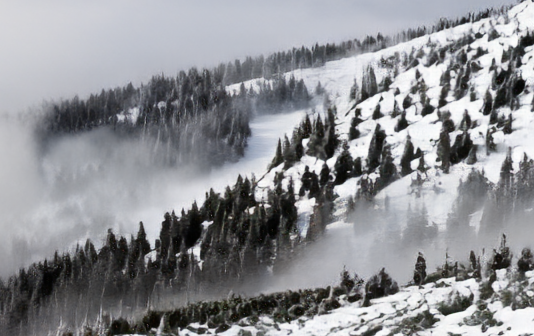
\includegraphics[width=\textwidth]{figure/forest-blurry.png}
    \caption{Example of an image compressed with Hyperprior module.}
    \label{forest-blurry}
\end{figure}

Images have following drawbacks:

\begin{enumerate}
    \item blurry
    \item noisy
\end{enumerate}

To overcome this issue we propose a novel approach: we include several super resolution layers in our generator. These layers remove blurry artifacts and make resulting images more sharp.

Image super resolution proposal can be formulated as a learning complex degradations from data. It is clear that the first step here is to produce a dataset from that a model then can be learned. Common choice here is to apply degradations on images before passing them into training pipeline.

We consider following degradations: blur, noise, downsampling, JPEG compression. Blur makes image less sharp and here traditional choice is gaussian blur kernel. Noise increases variance of image pixels, common choice is gaussian noise, which is sampled from gaussian distribution. Downsampling operation makes an mage smaller. There are several approaches to resize images: bilinear, bicubic and nearest neighbor interpolation.

For super resolution we use a common architecture, which has been used in \cite{Ledig_Theis_Huszar_Caballero_Cunningham_Acosta_Aitken_Tejani_Totz_Wang_et_al_2017}, \cite{Wang_Yu_Wu_Gu_Liu_Dong_Qiao_Loy_2019}, \cite{Wang_Xie_Dong_Shan_2021}. This architecture also is a fully convolutional net. Here we use a deep convolutional network body to extract meaningful features from an image (this network is 23 layers deep currently). We use residual connections for each layer of the network body. Each residual block performs four convolution operations, having features concatenated with all previous outputs channel-wise as it is shown on figure \ref{upscale}.

\begin{figure}[!ht]
    \centering
    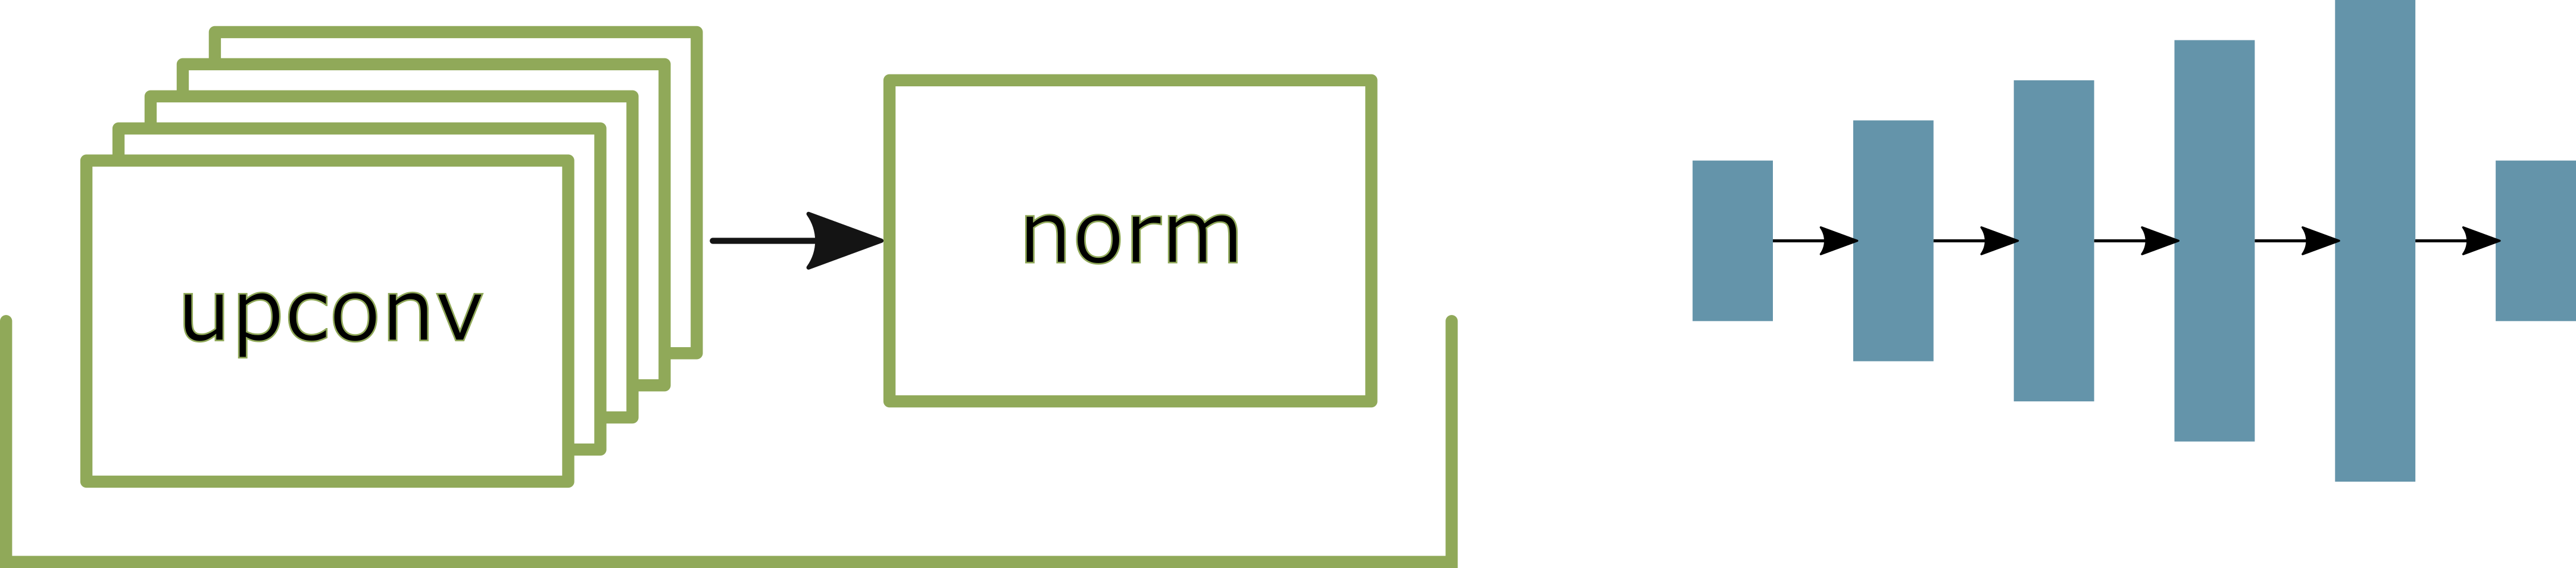
\includegraphics[width=\textwidth]{figure/upscale.png}
    \caption{For upscale we use a combination of convolution layers with residual connection (left). For visualization we also include channel dimensionality dynamics along the propagation through the convolutional layers (right).}
    \label{upscale}
\end{figure}

Having convolutional features propagated through the network body we apply two simple upsampling layers, that use a non-learnable interpolation operation and convolution layer followed by ReLU activation function.

We imply L1 loss \ref{eq:1}, L2 loss \ref{eq:2} and GAN losses from equations \ref{eq:loss-d} and \ref{eq:loss-g} to pretrain super resolution module. Afterwards we fine tune an entire framework. Using same loss functions mentioned above.

The last part of the framework is artifacts removal network. This network is a small enhancer placed on top of the described framework to further improve the quality of compressed and decompressed images. We tested several popular models and collected data from them. We show that this step may increase the restored image quality. We place enhancer module on top of the network and fine tune the entire model on our dataset.

For debluring and denoising we use a common architectures. We compare enhancement models \cite{zhang2017learning, zhang2020plug, jiang_towards_2021} in combination with our compression model to further improve image compression results.

The first model \cite{zhang2017learning} proposes a denoiser model that is capable of removing a noise artifacts from images.

The second model \cite{zhang2020plug} is an improved version of the first one, which is also denoiser.

The third model \cite{jiang_towards_2021} is a general artifact removing model. It is especially useful since it can work in blind manner, which means that no prior knowledge such as quantization table is required to perform a reconstruction and artifact removal.

\subsection{Training implementation}

To implement training pipeline we mentioned above, we use a famous PyTorch framework. Having our model we implement training of entire model using traditional GAN pipeline: we iterate over the data batches and each even batch we optimize a compression loss, each odd batch we optimize a GAN loss.

We use $3$ separate optimizers: one for Hyperprior probability model, another for compression model and the last one for GAN model. We use Adam optimizer as it is mentioned in the next section. First two optimizers are responsible for training the compression model. The last one is responsible for training the GAN model, which improves the performance of the reconstruction. And separately we also use the fourth optimizer to fine tune entire model with enhancement module. Enhancement modules are trained using their own pipelines and we do not describe it in this work.

Each compression training step we optimize compression loss from the formula \ref{eq:loss-eg}, and each GAN training step we optimize GAN loss from the formula $-log(D(x',y)$. This  statement ie essential for understanding of training our entire framework.

\chapter{Experiments}
\label{chapter:experiments}

\section{Data}
\label{section:data}

We used several datasets to train and test the models we've implemented. One is Visual Genome dataset, which has been used in many other works \cite{krishna_visual_2017}. Visual genome consists of more than 100,000 images labeled with scene graphs. We used Visual Genome for training scene graph based compression models.

Dataset consists of several main parts:

\begin{enumerate}
    \item Region descriptions. Human labeled important regions of an image, each description phrase is 1 to 16 words long.
    \item Objects. Objects labeled and canonicalized to a synset ID in WordNet.
    \item Attributes. Both images and objects have attributes. They are also canonicalized to WordNet.
    \item Relationships. Connects a pair of objects. Relationships are directed.
    \item Region graphs. A graph of a region of an image. These could be more than one region graph on one image.
    \item Scene graphs. A composition of region graph of an image. One image has exactly one scene graph.
    \item Question-answer pairs. There are both region-based and freeform QA pairs.
\end{enumerate}

It might be more adequate to split the Visual Genome dataset on the following general parts for better understanding:

\begin{enumerate}
    \item Images in JPEG format with various height and width.
    \item Detected objects information (coordinates of rectangles for each object, objects labels, objects attributes).
    \item Scene graphs, obtained from images.
\end{enumerate}

The dataset itself is quite big (more then 30 Gb), so we implemented a data loader that can work with such amounts of data. There were some efforts \cite{yang_2018_graph} to build a framework capable of working with the Visual Genome dataset, however there are no any stable version to work with.

Another dataset we use in this work is Open Images \cite{OpenImages2}. Open Images is a dataset of ~9M images annotated with image-level labels, object bounding boxes, object segmentation masks, visual relationships, and localized narratives:

\begin{enumerate}
    \item It contains a total of 16M bounding boxes for 600 object classes on 1.9M images, making it the largest existing dataset with object location annotations. The boxes have been largely manually drawn by professional annotators to ensure accuracy and consistency. The images are very diverse and often contain complex scenes with several objects (8.3 per image on average).
    \item Open Images also offers visual relationship annotations, indicating pairs of objects in particular relations (e.g. "woman playing guitar", "beer on table"), object properties (e.g. "table is wooden"), and human actions (e.g. "woman is jumping"). In total it has 3.3M annotations from 1,466 distinct relationship triplets.
    \item In V5 we added segmentation masks for 2.8M object instances in 350 classes. Segmentation masks mark the outline of objects, which characterizes their spatial extent to a much higher level of detail.
    \item In V6 we added 675k localized narratives: multimodal descriptions of images consisting of synchronized voice, text, and mouse traces over the objects being described. (Note we originally launched localized narratives only on train in V6, but since July 2020 we also have validation and test covered.)
    \item Finally, the dataset is annotated with 59.9M image-level labels spanning 19,957 classes.
\end{enumerate}

The KODAK \cite{kodak} dataset is yet another popular choice for image compression evaluation. This dataset is fairly small and contains a non-compressed true color PNG images.

CLIC \cite{noauthor_clic_nodate} is a dataset for the Challenge on Learned Image Compression 2020 lossy image compression track. These images contain a mix of the professional and mobile datasets used to train and benchmark rate-distortion performance. The dataset contains both RGB and gray scale images. This may require special handling if a gray scale image is processed as a 1 channel Tensor and a 3 channel Tensor is expected.

\section{Training}

We trained our networks with different configurations and evaluated it on separate dataset. We use Open Images \cite{OpenImages2} for training. It is a a huge dataset of 9 million images. Those images are annotated with image-level and object-level annotations, bounding boxes, visual relations and segmentation masks. We use this dataset to train and test models of image compression, which means we do only need clean images without annotations. We use near 150,000 images subset from 9,000,000 images dataset. This amount is sufficient to train a compression model.

We evaluate our model on KODAK \cite{kodak} dataset. The pictures from this dataset are lossless compressed, true color (24 bits per pixel, aka "full color") images in PNG format. This dataset is a very common choice in image compression models evaluation, since the images from that dataset are given in high quality and have various structure.

\subsection{Pretraining autoencoder}

We start training from autoencoder (no GAN). It takes $1.5$ hour to complete one epoch on Nvidia TESLA K80. We complete $10$ epochs to train an autoencoder. However, the autoencoder even after training has a noisy artifacts (figure \ref{training-compression-examples}), that will be fixed on the next stages.

\begin{figure}[!ht]
    \centering
    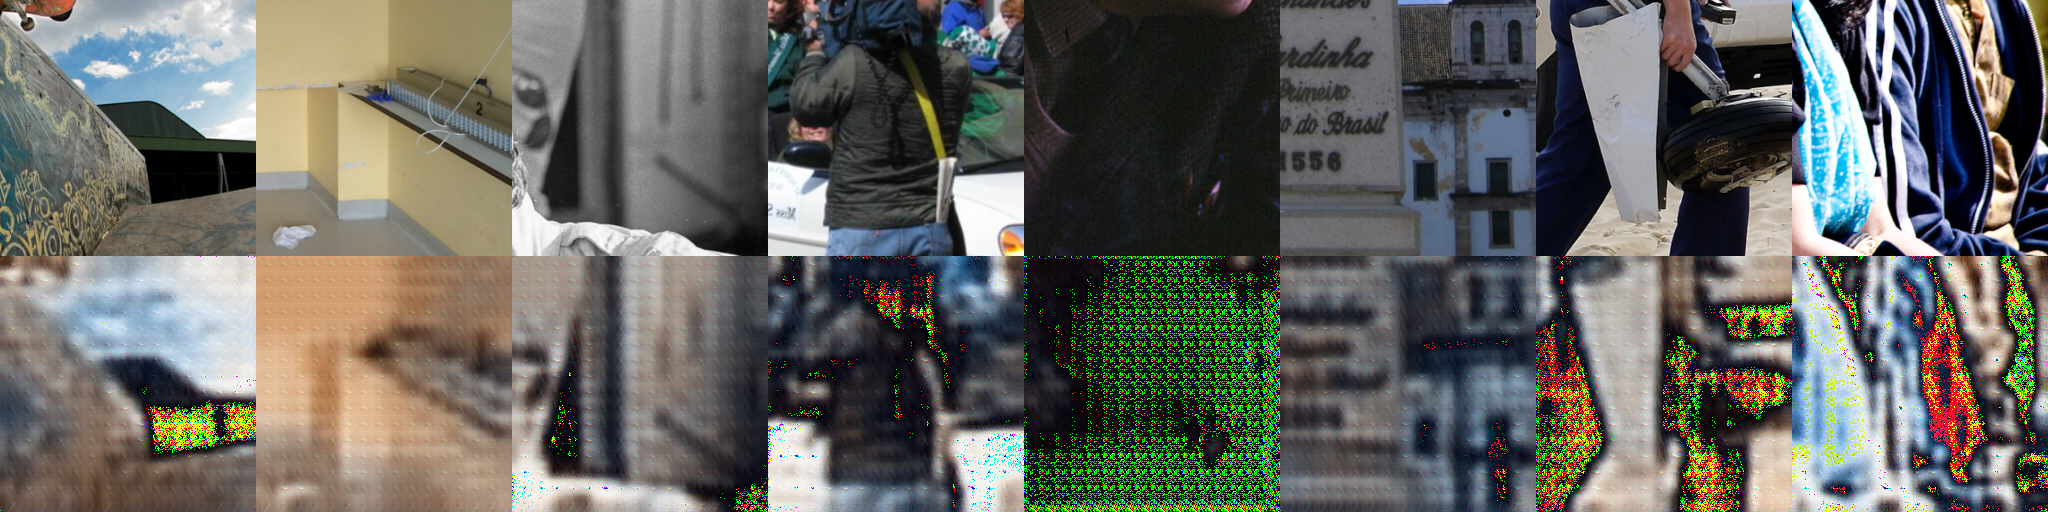
\includegraphics[width=\textwidth]{figure/step_1000.png}
    a) First epoch
    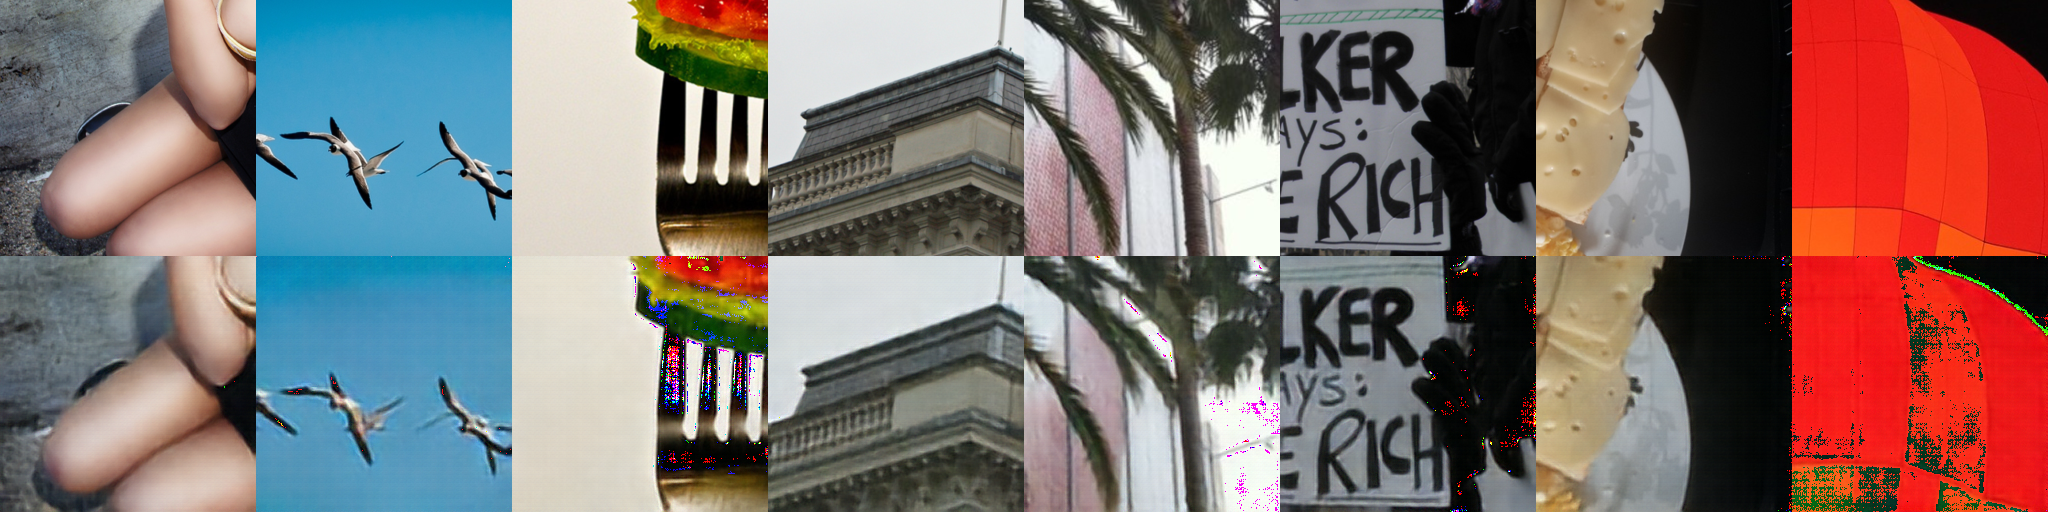
\includegraphics[width=\textwidth]{figure/step_15000.png}
    b) Second epoch
    \caption{Training process of compression model (no GAN). The first set of pictures (a) displays the images state after the first epoch of training. The second set of pictures (b) displays the images state after the second epoch of training.}
    \label{training-compression-examples}
\end{figure}

Compression is optimized on this step. This means that the compressed representation size is optimized to be smaller and smaller each step (figure \ref{training-compression-q-rate}).

\begin{figure}[!ht]
    \centering
    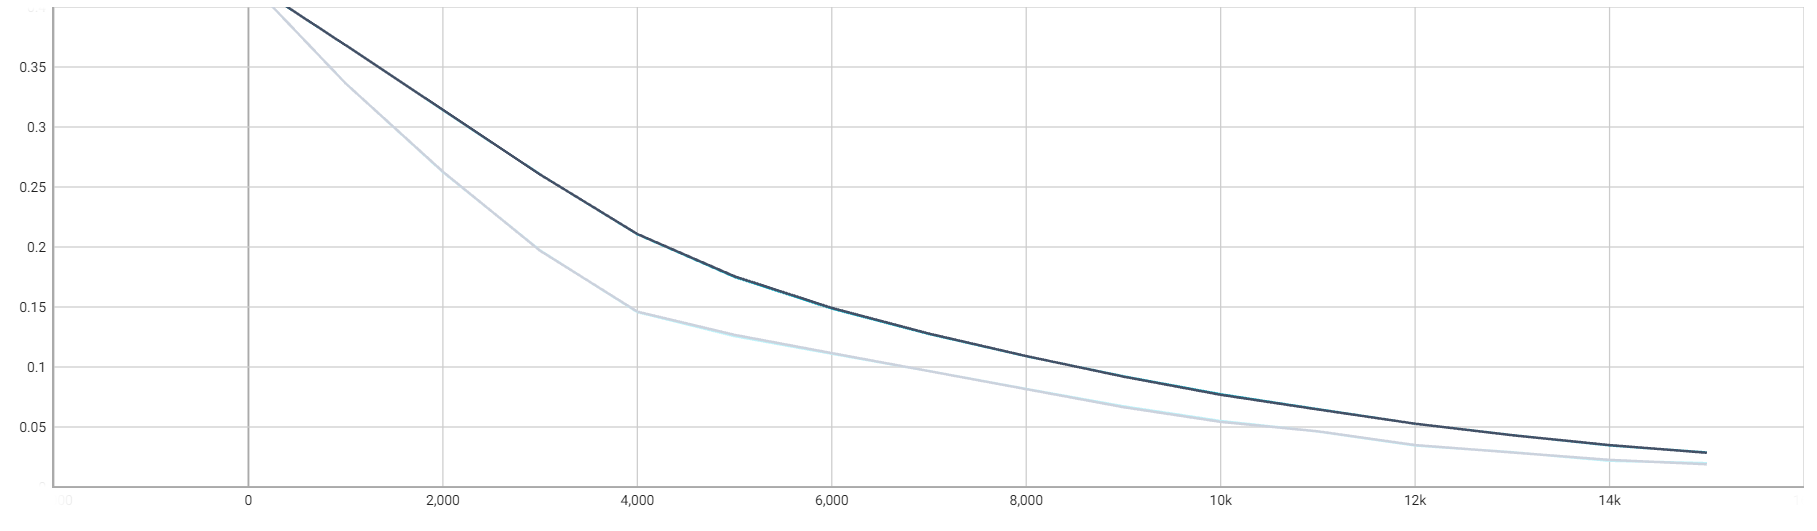
\includegraphics[width=\textwidth]{figure/compression-q-rate-hyperlatent.png}
    \caption{The hyperlatents compression rate.}
    \label{training-compression-q-rate}
\end{figure}

We see that compression rate is optimized much more easy than the reconstruction images quality.

\subsection{GAN}

The next stage of training is adversarial training. On this stage we not only optimize autoencoder loss, but also put the discriminator on top of the autoencoder network and optimize the network in GAN manner. This means that we split the training iteration on two steps: compression model step and GAN step.

One training epoch of GAN model takes up to $3$ hours on Nvidia TESLA K80. We complete $10$ such epochs.

The GAN loss is displayed on figure \ref{training-compression-gan-discriminator}.

\begin{figure}[!ht]
    \centering
    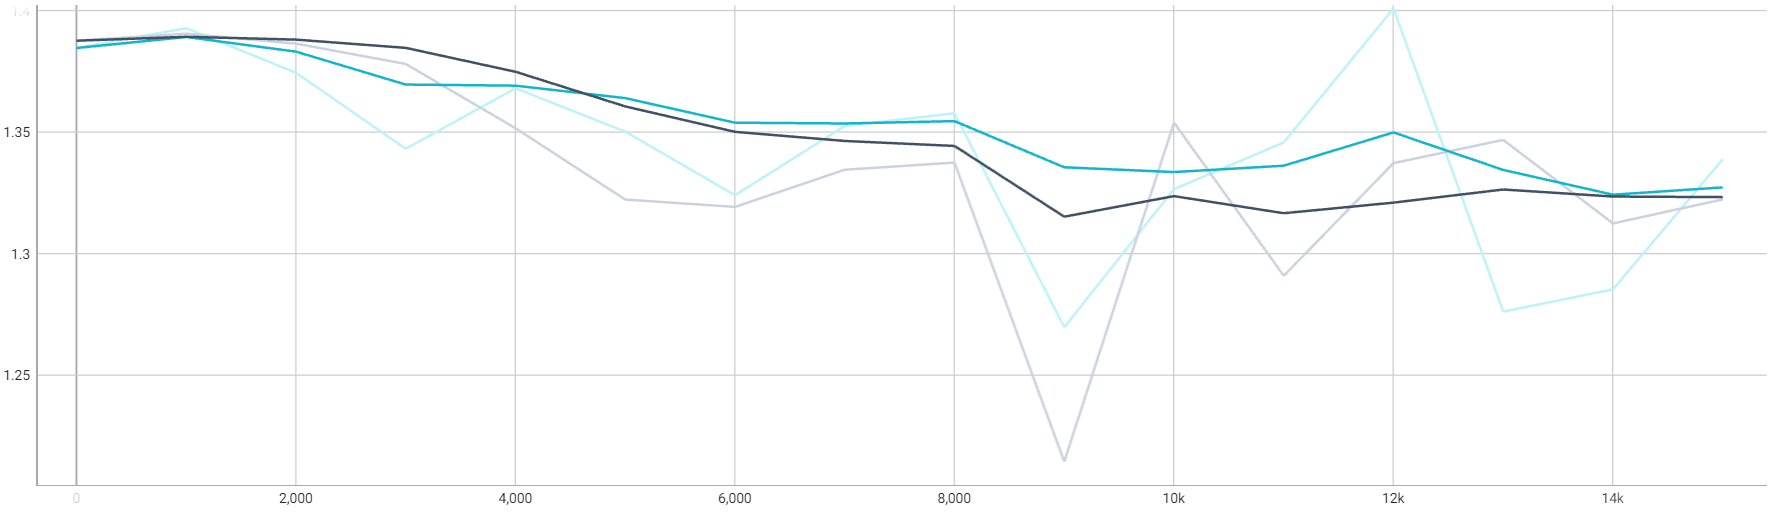
\includegraphics[width=\textwidth]{figure/compression-gan-discriminator.png}
    \caption{The GAN loss.}
    \label{training-compression-gan-discriminator}
\end{figure}

As we can see from the figure, the loss converges not as well as in compression autoencoder model. This is probably due to the fact that the model is overcomplicated and we already have a pretrained compression model, which weights are already ner local minima, but GAN weights are not. Anyways, the sufficient number of epochs resolves this issue, and converges the loss, but more slowly than the compression autoencoder model.

\begin{figure}
    \centering
    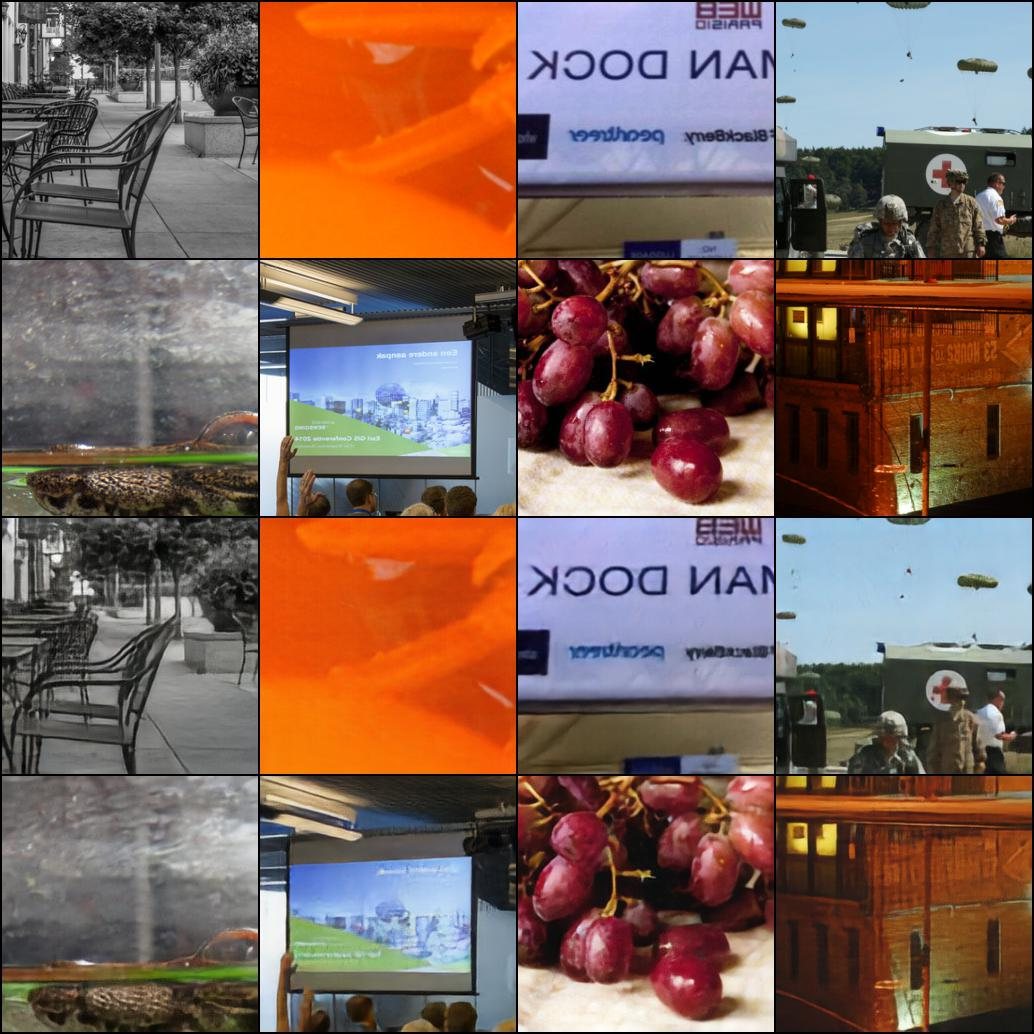
\includegraphics[width=\textwidth]{figure/gan_1000.jpg}
    \caption{The images after training first epoch with GAN loss.}
    \label{gan-first-epoch}
\end{figure}

When we first tried the GAN version of the model, we also oriented on the loss and were disappointed with the result. However, it's important to mention that the actual results of compressed images are much better than the loss figure shows. This is one side of a more complex problem. It is difficult to define a good loss function for image compression and restoration, especially to define, how different are two images. We described some of the approaches in the previous chapter.

\begin{figure}
    \centering
    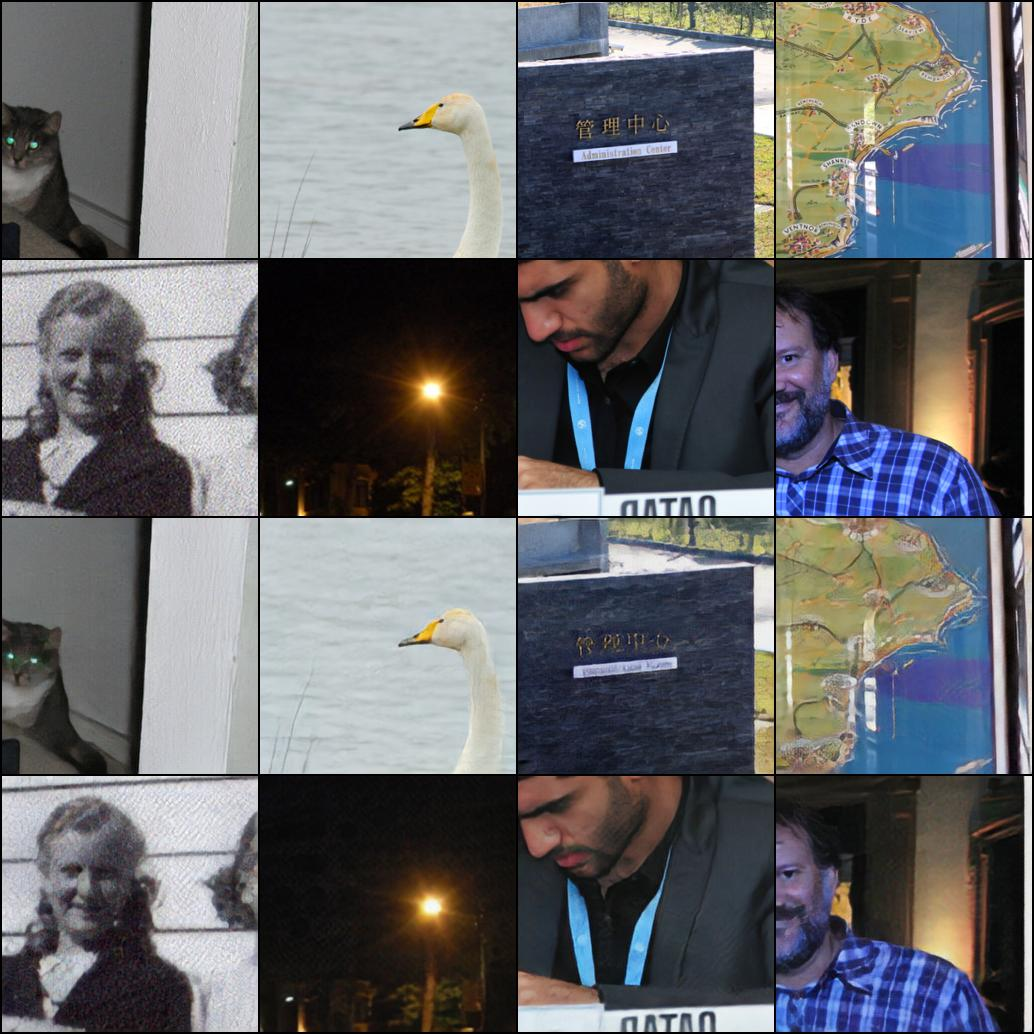
\includegraphics[width=\textwidth]{figure/gan_14000.jpg}
    \caption{The images after training 10th epoch with GAN loss.}
    \label{gan-tenth-epoch}
\end{figure}

As we clearly see, the performance of a model grows with more training. GAN makes the image smoother and removes noise artifacts. However, noise is still a thing in these images. This is why we do not stop on this step, but also append several enhancement layers on top of our network.

\subsection{Fine tuning with enhancement models}

To fine tune enhancement models we first pretrain these models on dataset. Then we use our compression model as a source of input data e.g. we place enhancer on top of the model and fine tune the model like this.

\section{Training settings}

We set $\lambda$ to $1$ and $\beta$ to $0.15$ parameters from \ref{eq:loss-g}. We set a learning rate of $10^{-4}$ and train the network using Adam optimizer \cite{kingma_adam_2017} with weight decay $10^{-6}$, $\beta_1 = 0.9$, $\beta_2 = 0.999$. We train the networks in 2 steps: first step is training compression and upscale networks in GAN manner (using generator and discriminator losses), the second step is to fine tune them together.

By increasing and decreasing $\beta$ and $\lambda$ we can control a tradeoff between compression and distortion loss terms on the training stage. This allows us to select a better hyperparameter for the network. The process of hyperparameter selection is following: start training network and after some number of iterations (we usually wait few epochs) we compare the results of validation dataset. If this set of hyperparameters performs better than previous set, we should use this one.

\begin{figure}[!ht]
    \centering
    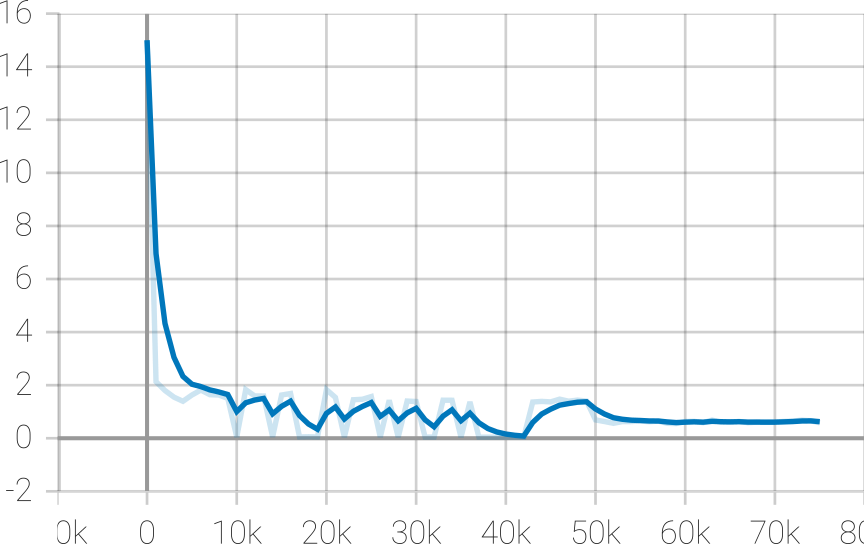
\includegraphics[width=0.3\textwidth]{figure/weighted_compression_weighted_rate.png}
    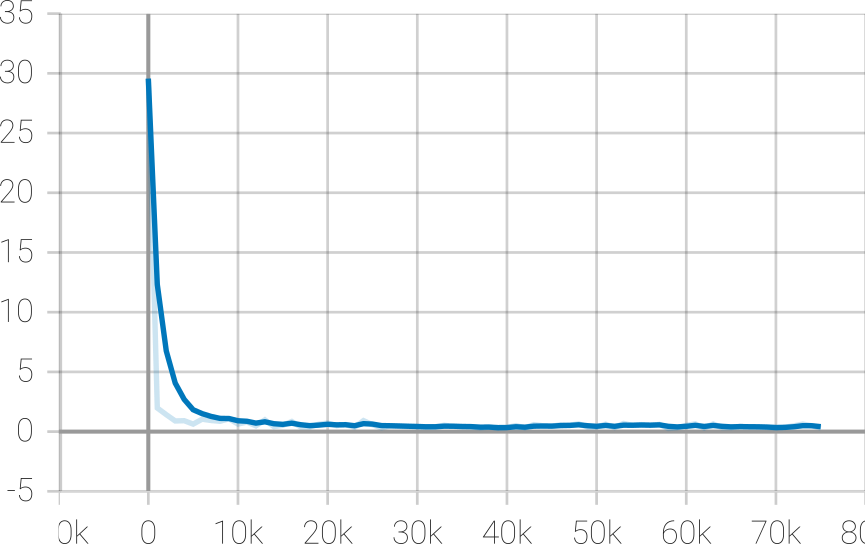
\includegraphics[width=0.3\textwidth]{figure/weighted_compression_weighted_distortion.png}
    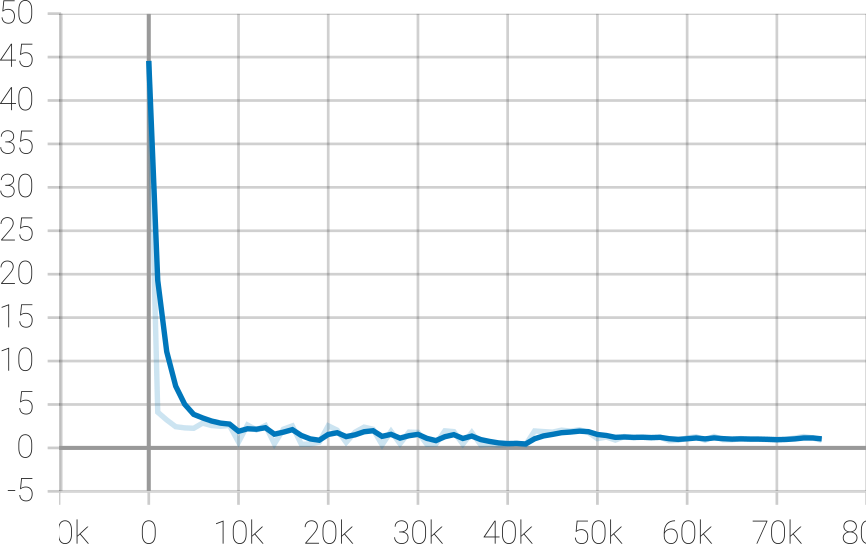
\includegraphics[width=0.3\textwidth]{figure/weighted_compression_weighted_R_D.png}
    \caption{Training process for compression module. As we can see, compression rate term (left) and distortion term (middle) in combination give final rate/distortion loss (right).}
    \label{compession-losses}
\end{figure}

It is clear from the figure \ref{compession-losses}, how compression and distortion losses in combination together give final loss term \ref{eq:loss-egp}.

\section{Metrics}

For evaluation we use different existing metrics and also propose a novel metric that supposedly better reflect the performance of compression models. The metrics we use in our work are Multi-Scale Structural Similarity (MS-SSIM), Pike Signal to Noise Ratio (PSNR), BPP (Bits Per Pixel).

\subsection{Multi-Scale Structural Similarity}

Multi-Scale Structural Similarity (MS-SSIM) is a metric that measures similarity between two images. It measures a relative similarity between two images based on statistics such as mean $\mu$, mean squared error $\sigma$ \ref{eq:ms-ssim}.

\begin{equation}
    \label{eq:ms-ssim}
    \begin{split}
        l(x, y) = \frac{2\mu_x\mu_y + C_1}{\mu_x^2 + \mu_y^2 + C_1},\\
        c(x, y) = \frac{2\sigma_x\sigma_y + C_2}{\sigma_x^2 + \sigma_y^2 + C_2},\\
        s(x, y) = \frac{\sigma_{xy} + C_3}{\sigma_x\sigma_y + C_3},\\
        SSIM(x, y) = [l_M(x, y)]^{\alpha_M} * \prod_{j=1}^{M}[c_j(x, y)]^{\beta_j}[s_j(x, y)]^{\gamma_j}
    \end{split}
\end{equation}

Where $x$ is the first image and $y$ is the second image, $\mu_x$ is mean of $x$ and $\mu_y$ is mean of $y$, $\sigma_x$ is mean squared error of $x$ and $\sigma_y$ is mean squared error of $y$, $\sigma_{xy}$ is covariance between $x$ and $y$. $l(x, y)$ is luminance similarity component, $c(x, y)$ is color similarity and $s(x, y)$ is structure similarity. $\alpha$, $\beta$ and $\gamma$ are weights of these components. $C_1$, $C_2$, $C_3$ are adjustable coefficients.

\subsection{Pike Signal to Noise Ratio}

Pike Signal to Noise Ratio (PSNR) is a term that is used to measure the quality of an image. More precise it shows the ratio between the maximum signal power and maximum noise power in concrete image. This metrics is usually used in lossy image or video compression to evaluate the compression models based on the quality of reconstructed images.

PSNR is defined using mean squared error term (MSE) \ref{eq:mse}.

\begin{equation}
    \label{eq:mse}
    \mathit{MSE} = \frac{1}{m,n} \sum _{i=0}^{m-1} \sum _{j=0}^{n-1} [I(i,j)-\hat{I}(i,j)]^{2}
\end{equation}

The PSNR (in dB) is defined in equation \ref{eq:psnr}

\begin{equation}
    \label{eq:psnr}
    \begin{aligned}
        \mathit {PSNR} & = 10 * log_{10} \left(\frac{\mathit{{MAX}_{I}^{2}}}{\mathit {MSE}} \right)   \\
                       & = 20 * log_{10} \left(\frac{\mathit{{MAX}_{I}}}{\sqrt{\mathit{MSE}}} \right) \\
                       & = 20 * log_{10}(\mathit{{MAX}_{I}}) - 10 * log_{10}(\mathit{MSE})
    \end{aligned}
\end{equation}

Where $MAX_I$ is the maximum possible pixel value of the image. When the pixels are represented using $8$ bits per sample, this is $255$. More generally, when samples are represented using linear PCM with $B$ bits per sample, $MAX_I$ is $2B − 1$.

\subsection{Bits Per Pixel}

When we want to measure the effectiveness of image compression it is also important to take into account the compression power of a model in the concrete image setting. To further do it, we can employ a Bits Per Pixel (BPP) metrics, which shows an average number of bits required to store one pixel in compressed representation.

Image compression algorithms and image compression models different BPP ratio, image that is raw (not compressed) has a fixed amount of bits per each pixel of this image. However after  the compression procedure we have a smaller amount of bits required to store a concrete pixel.

\begin{equation}
    \label{eq:bpp}
    \mathit{BPP} = \frac{N}{P}
\end{equation}

Where $N$ is the amount of memory required to store the image, $P$ is the number of pixels in the image.

In traditional image compression algorithms like JPEG we have a fixed compression rate, which we can only calculate \textit{posteriori}.

In our work we calculate an actual bitrate of all compressed images. This means that even though the model is targeted to compress the images with some fixed bitrate, we still get different bitrate for different images, and, in most of the cases this bitrate is even smaller than the model was trained for.

\section{Evaluation and analysis}

We evaluate our data on separate dataset. We use three available target compression rates and produce metric that we described in the previous section. On the first figure \ref{mssim} we can see MS-SSIM metric. The horizontal axis is bitrate. We plot two differently measured bitrate: actual mean BPP, which is, as we described in the previous section, a more adequate metrics to measure a real performance of the network; and the target BPP, which is the BPP the model is targeted to reach.

\begin{figure}[!ht]
    \centering
    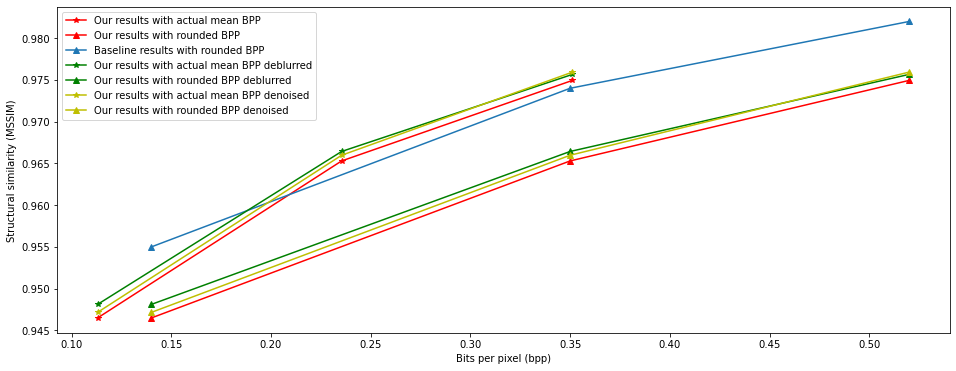
\includegraphics[width=\textwidth]{figure/mssim.png}
    \caption{MS-SSIM metrics we got during our experiments}
    \label{mssim}
\end{figure}

The second important metric is PSNR, also described in the previous section.

\begin{figure}[!ht]
    \centering
    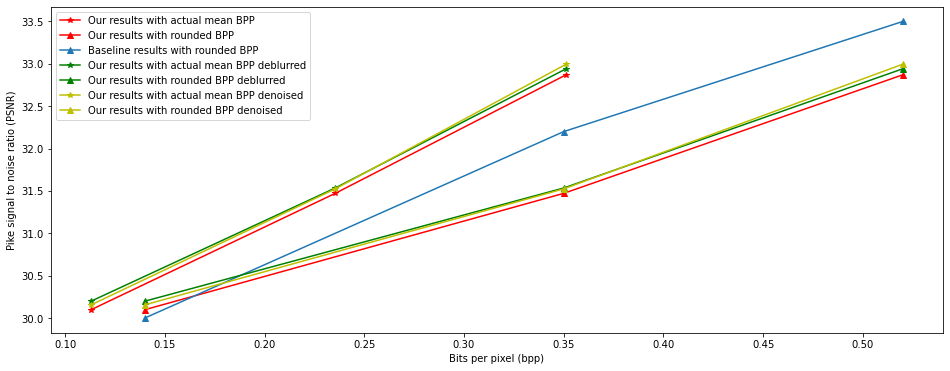
\includegraphics[width=\textwidth]{figure/psnr.png}
    \caption{PSNR metrics we got during our experiments}
    \label{psnr}
\end{figure}

As we can see from the figures \ref{mssim} and \ref{psnr}, the actual mean bitrate is way smaller than the target model bitrate. Of course, for each image the actual bitrate is less than target model bitrate. This is the reason we also use an actual mean BPP to evaluate the performance of the model. We think that this approach is more correct.

\subsection{Subjective results and Ablation study}

The images compressed with the use of original HiFiC model are more noisy. This is especially clear from the patches taken from low frequency areas. As we state in previous sections we resolve this issue by fine tuning the model with image enhancement models.

We first take a look at whole images. There is a picture of a jungle, where we can see the borders of objects (leafs) are better on our proposed model generated images.

\begin{figure}[!ht]
    \centering
    \begin{tabular}{cc}
        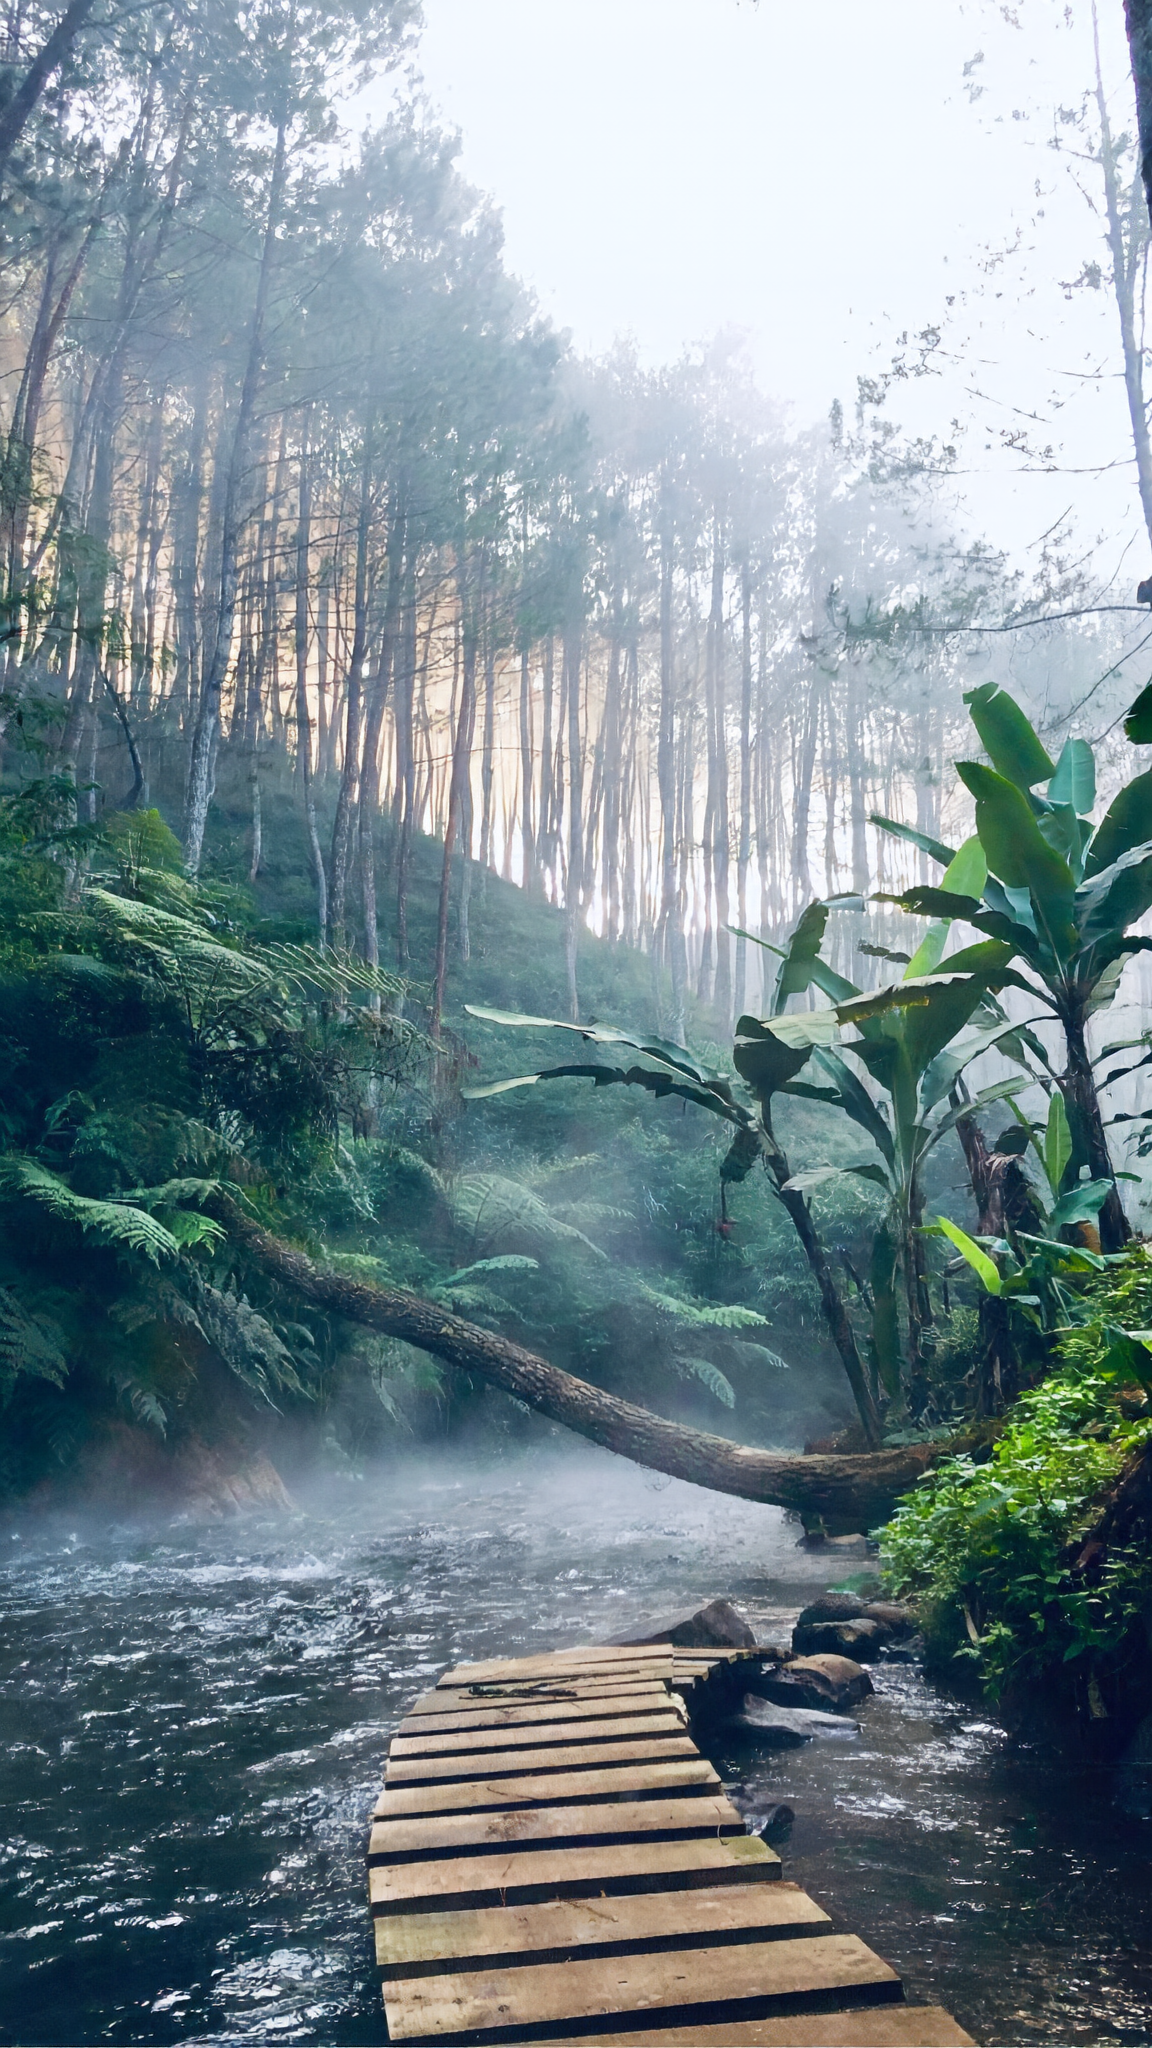
\includegraphics[width=0.4\textwidth]{figure/jungle-full.png} & 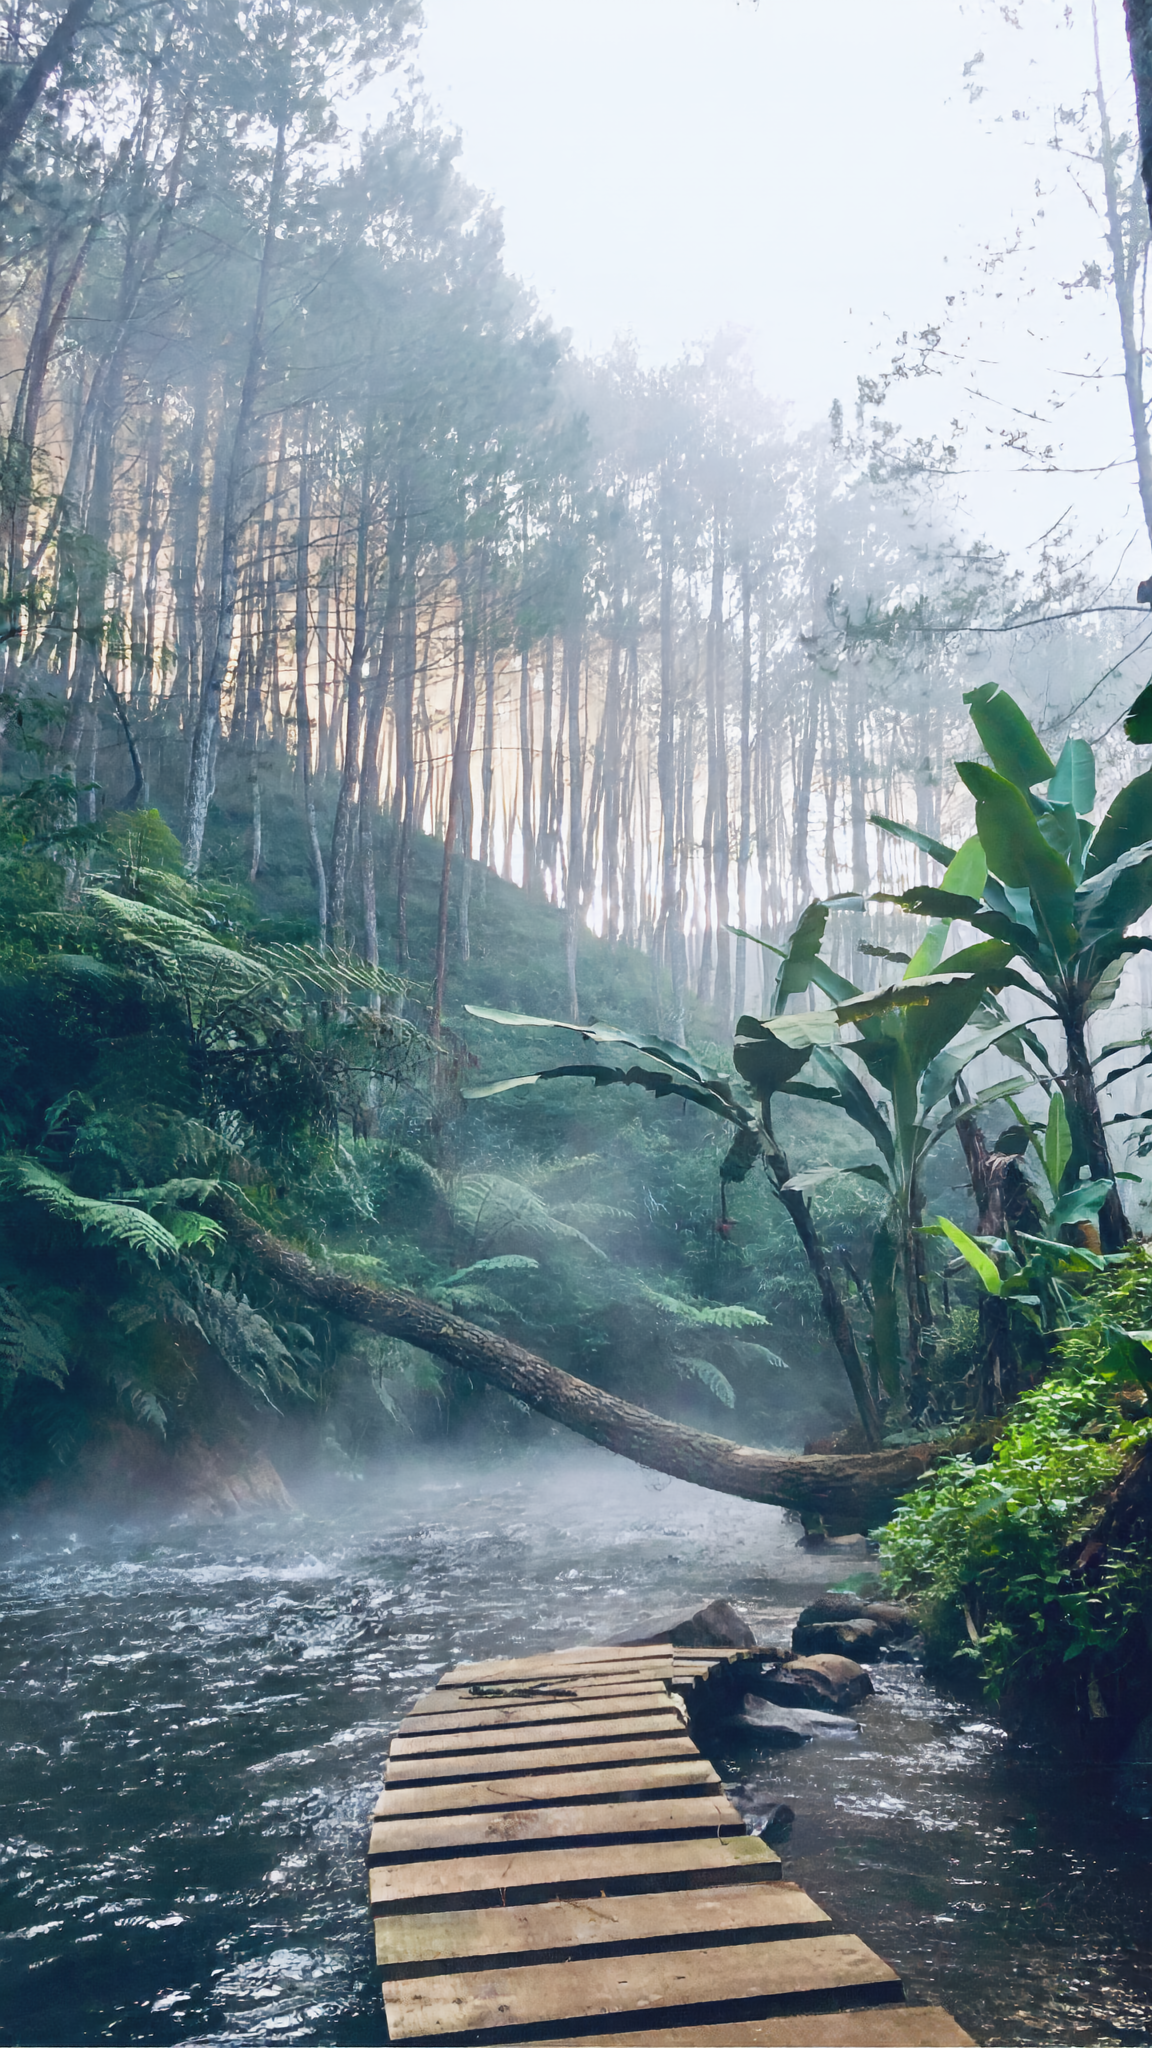
\includegraphics[width=0.4\textwidth]{figure/jungle-denoise-full.png} \\
        a) Baseline compressed                                        & b) Proposed model compressed
    \end{tabular}
    \caption{Images compressed with baseline HiFiC model and proposed model.}
    \label{compressed-jungle}
\end{figure}

On the picture of the sky we can clearly see that the low frequency areas of an images compressed with baseline model are also more noisy tan proposed model compressed images.

\begin{figure}[!ht]
    \centering
    \begin{tabular}{cc}
        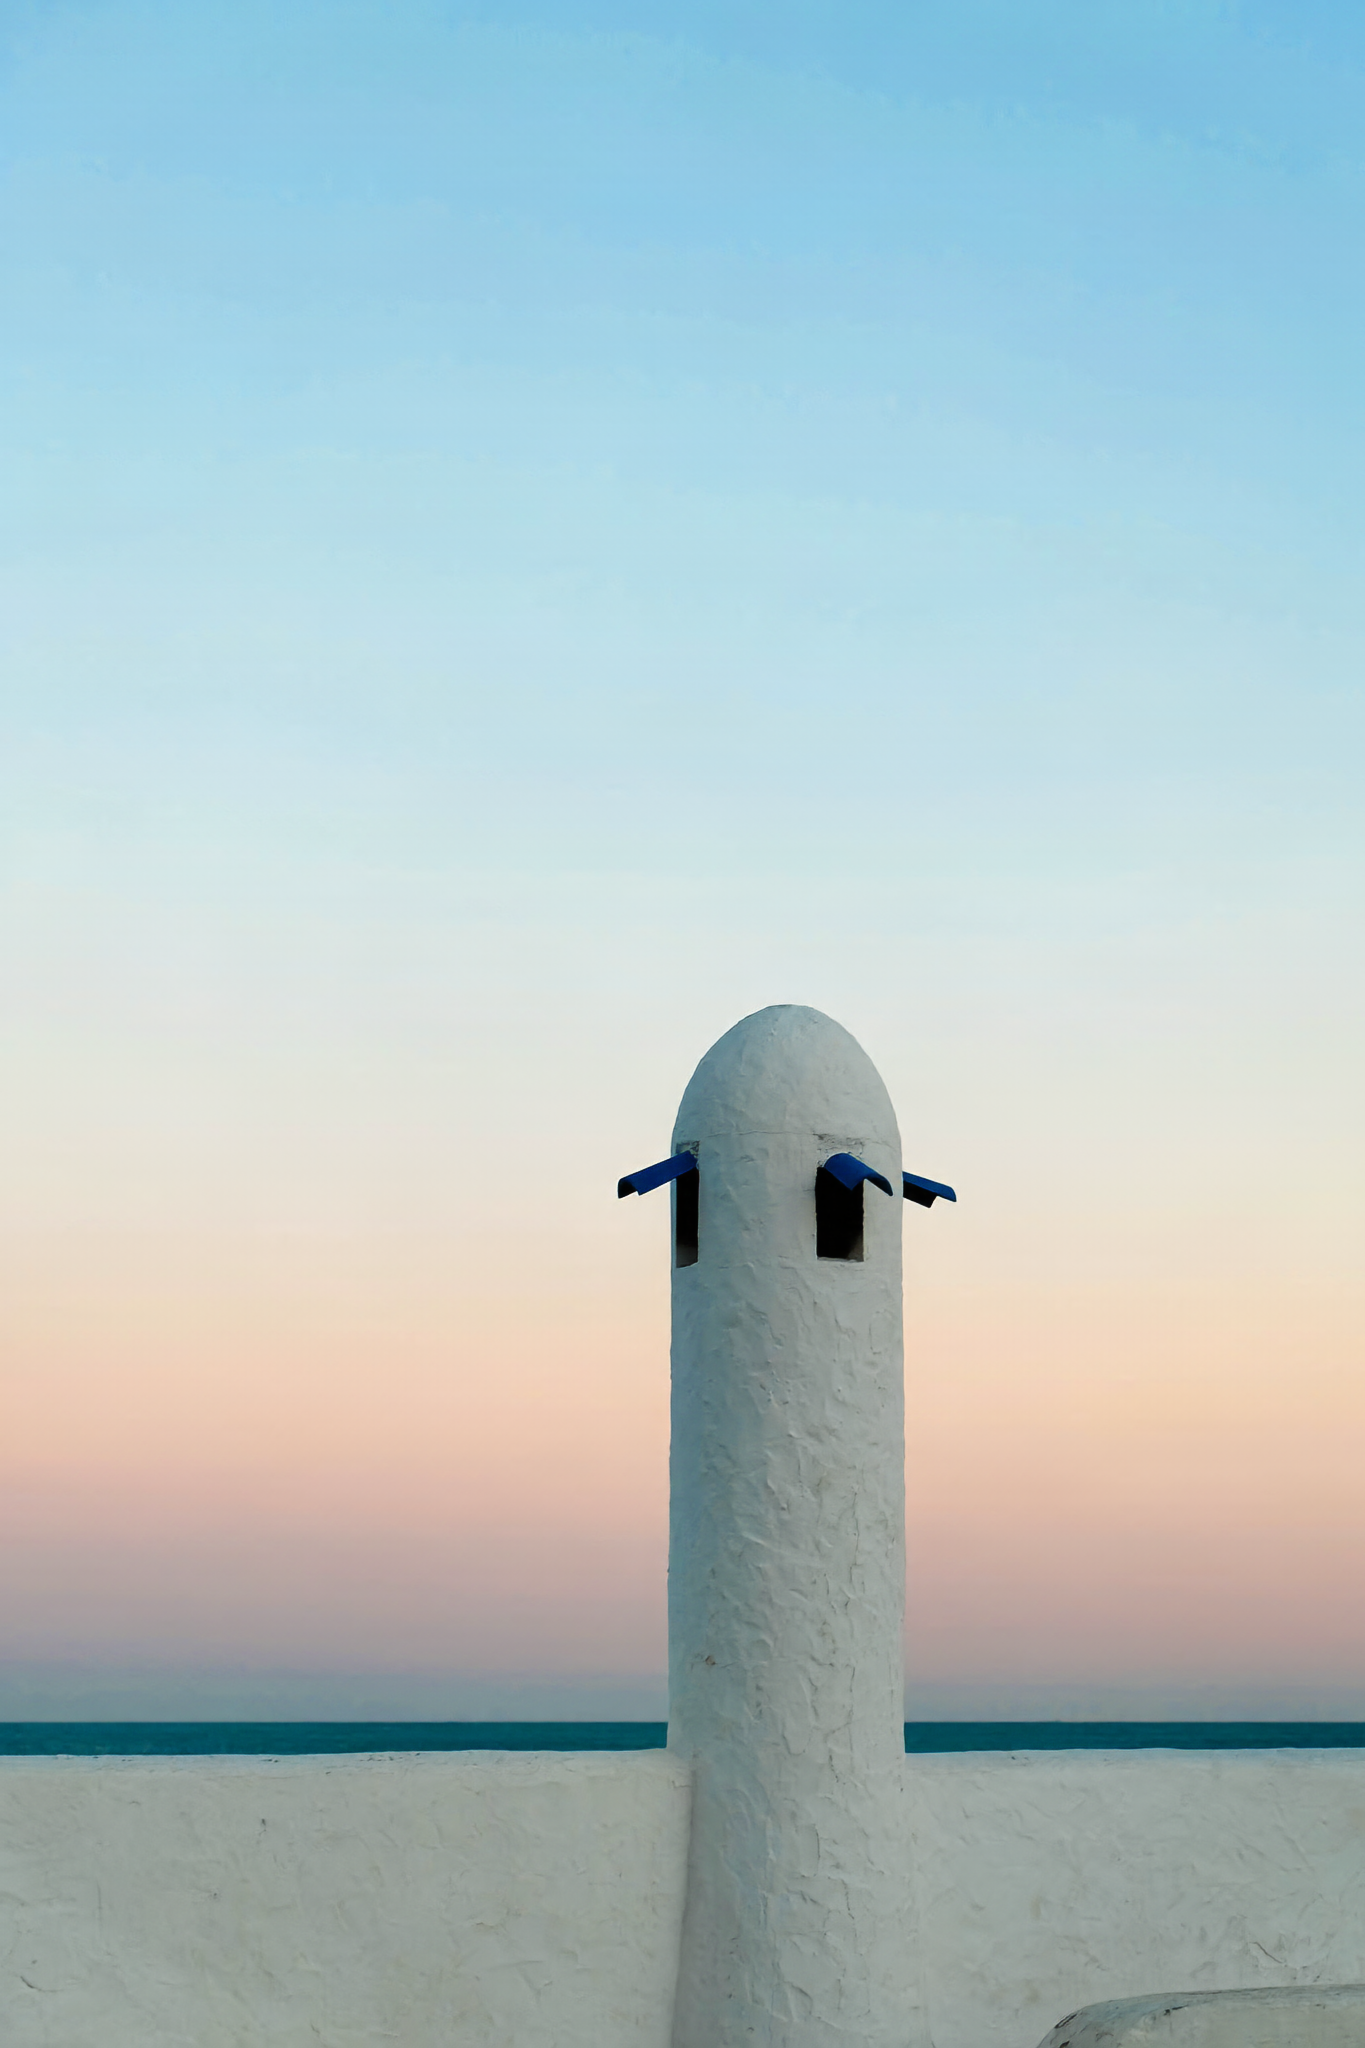
\includegraphics[width=0.4\textwidth]{figure/sky-recon-full.png} & 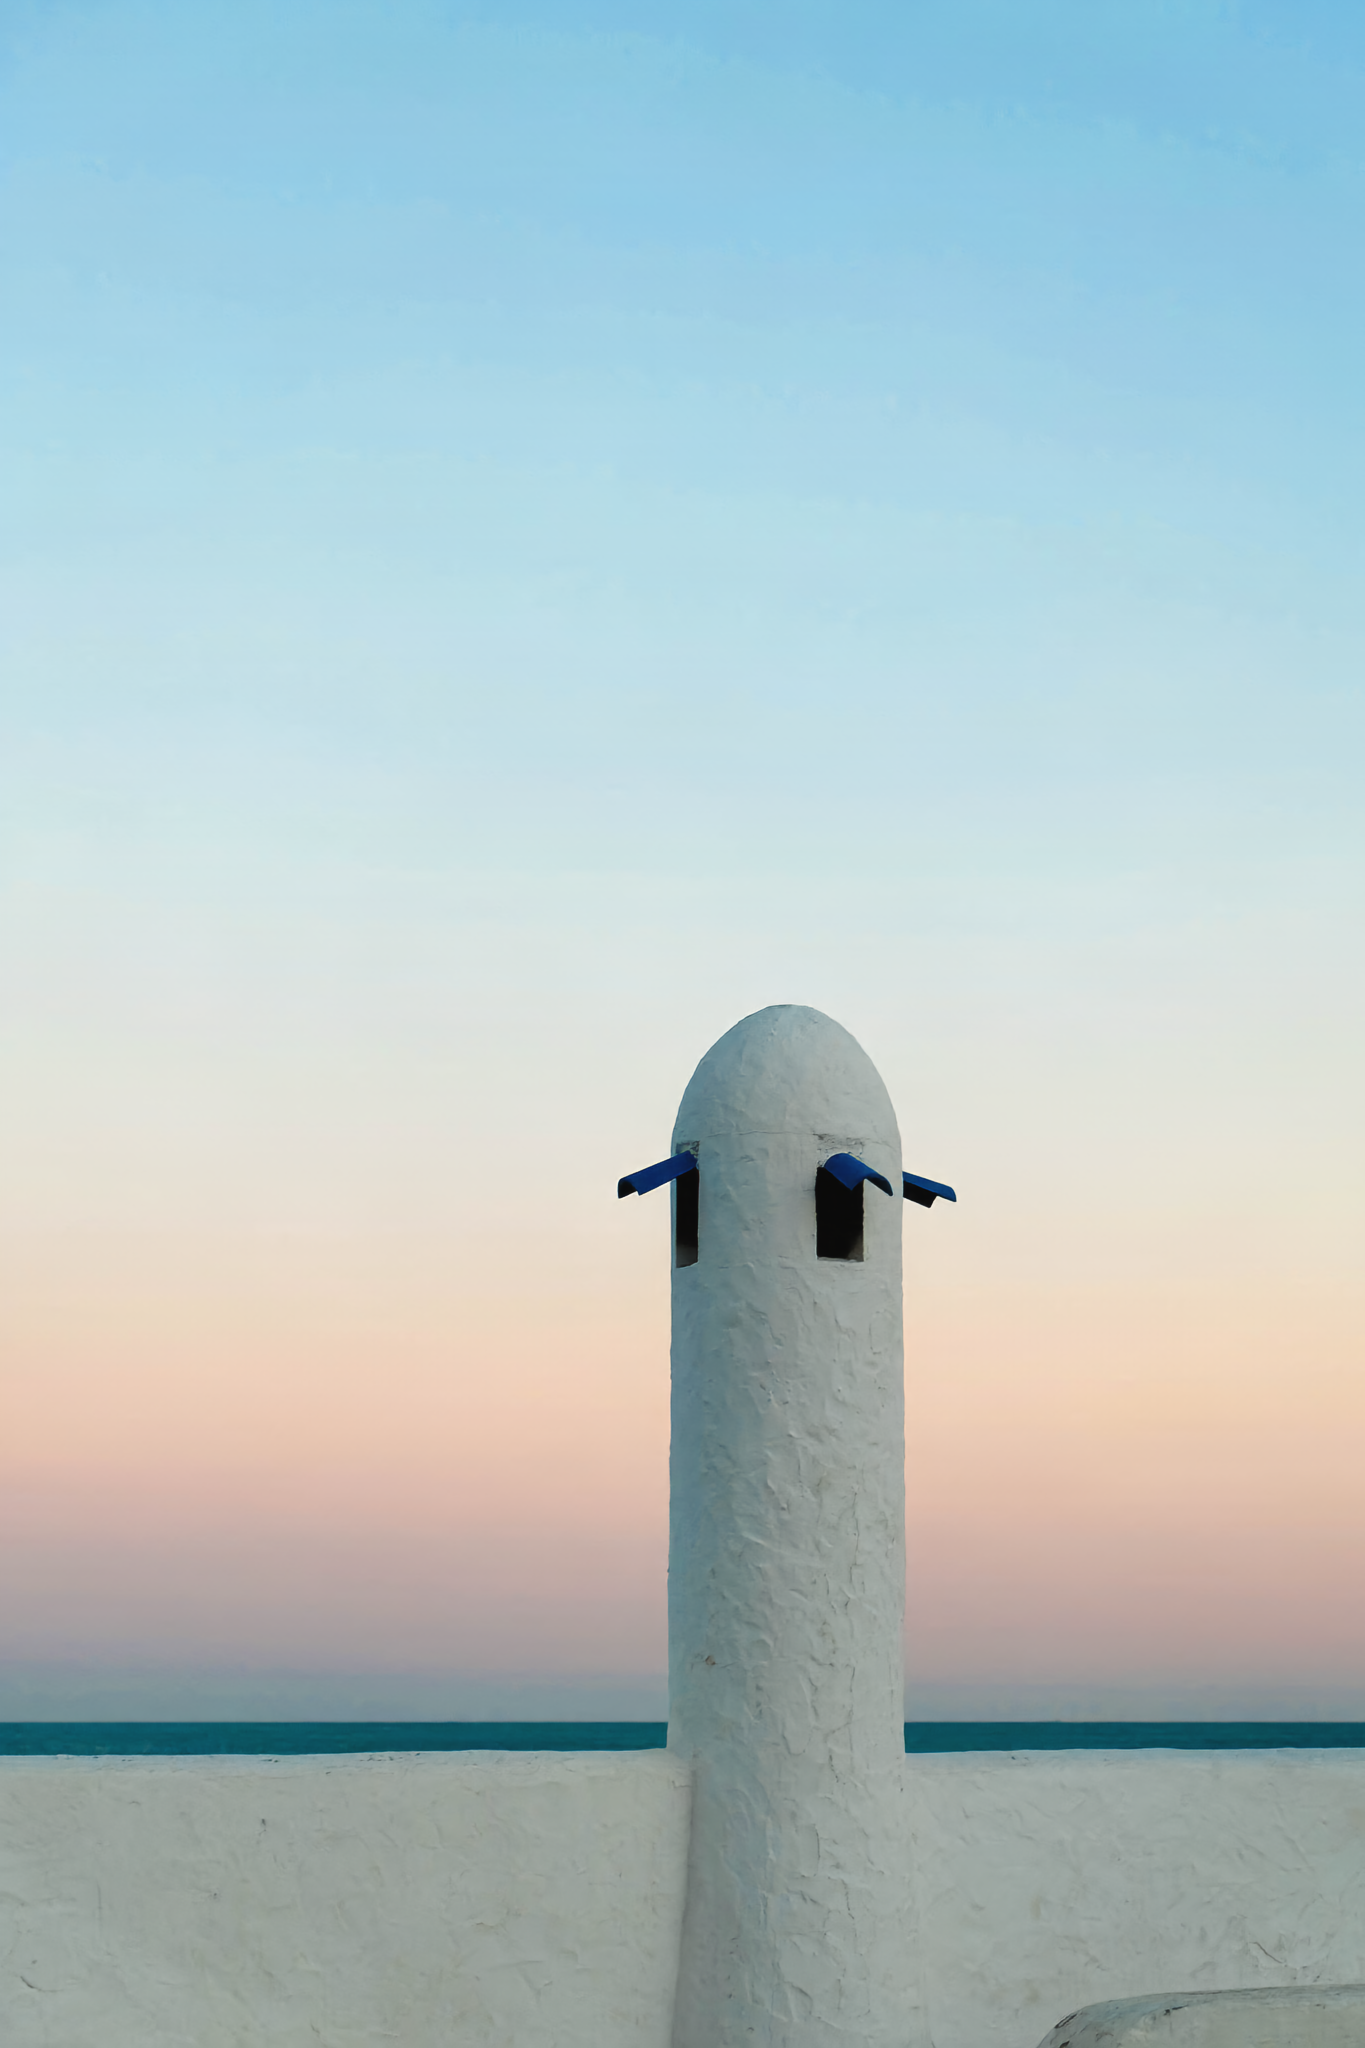
\includegraphics[width=0.4\textwidth]{figure/sky-recon-denoise-full.png} \\
        a) Baseline compressed                                           & b) Proposed model compressed
    \end{tabular}
    \caption{Images compressed with baseline HiFiC model and proposed model.}
    \label{compressed-sky}
\end{figure}

From the previous figures it may be unclear without zoom, what is the difference. However, we can zoom in and compare patches from some areas of the images.

\begin{figure}[!ht]
    \centering
    \begin{tabular}{cc}
        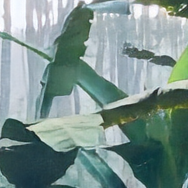
\includegraphics[width=0.4\textwidth]{figure/jungle-recon.png} & 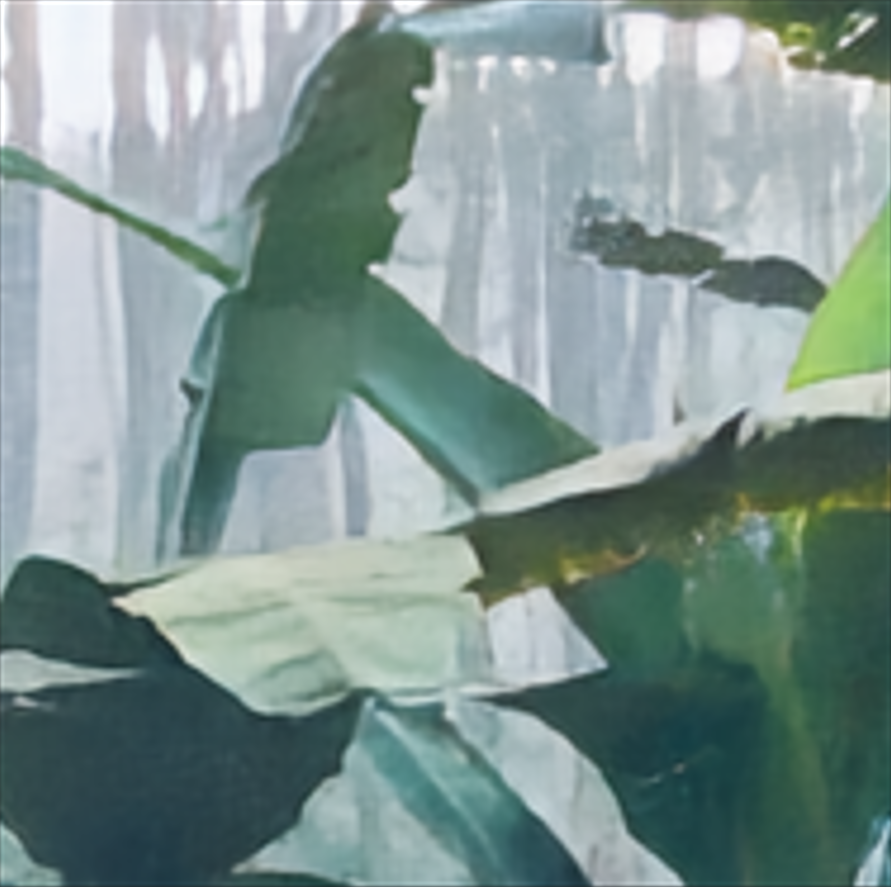
\includegraphics[width=0.4\textwidth]{figure/jungle-recon-denoise.png} \\
        a) Baseline compressed                                         & b) Proposed model compressed                                           \\
        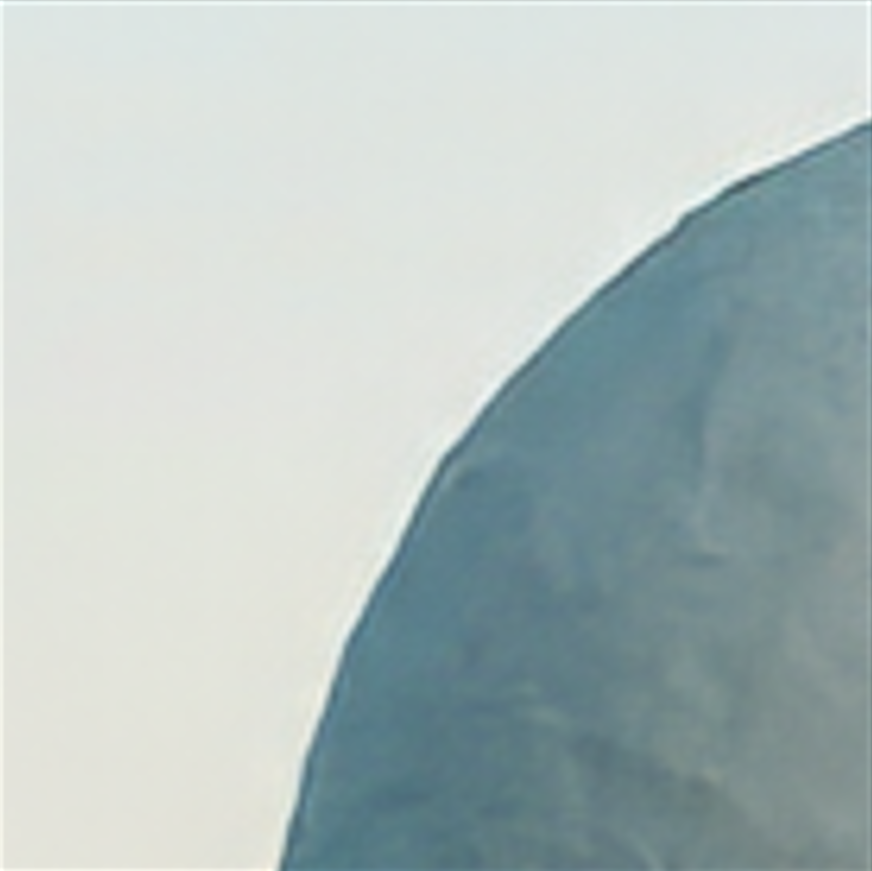
\includegraphics[width=0.4\textwidth]{figure/sky-recon.png}    & 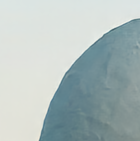
\includegraphics[width=0.4\textwidth]{figure/sky-recon-denoise.png}    \\
        c) Baseline compressed                                         & d) Proposed model compressed
    \end{tabular}
    \caption[Patches from images.]{These patches show how image enhancement network increases the quality of the images. (a) and (b) are the HiFiC compressed images, (c) and (d) are proposed model compressed images.}
    \label{patches}
\end{figure}

From the figure \ref{patches} we can see that the images processed with our model have less noise and better object borders.

\subsection{Model size analysis}

Since the residual layers of HiFiC \cite{mentzer_high_fidelity_2020} are quite heavy, we experimented with the number of these layers in the model. The original model contained $9$ residual layers in the generator. We managed to reduce the number of these layers, which lead to decreasing the number of parameters and therefore the generator module size by almost $43\%$.

We show three generator settings. As we can see from the table \ref{tab:generator}, we managed to decrease the number of residual layers, which lead to reasonable memory usage reduction.

\begin{table}
    \centering
    \caption{Generator with different number of the residual layers.}
    \label{tab:generator}
    \begin{tabular}{p{3cm}|p{2cm}|p{2cm}|p{4cm}}
        \hline
        \textbf{Number of residual layers} & \textbf{Total parameters} & \textbf{Parameters size (Mb)} & \textbf{Forward/backward pass size with input shape (3, 128, 128) (Mb)} \\
        \hline
        5 \textbf{(ours)}                  & 90,373,083                & 344.75                        & 79.43                                                                   \\
        \hline
        7                                  & 123,554,523               & 471.32                        & 87.04                                                                   \\
        \hline
        9 \textbf{(baseline)}              & 156,735,963               & 597.90                        & 94.66
    \end{tabular}
\end{table}

And from the table \ref{tab:model} we can see that model size has decreased by almost $37\%$. This is significant.

\begin{table}
    \centering
    \caption{Encoder}
    \label{tab:model}
    \begin{tabular}{p{4cm}|p{4cm}|p{4cm}}
        \hline
        \textbf{Module} & \textbf{Total parameters} & \textbf{Parameters size (Mb)} \\
        \hline
        Encoder         & 7,419,700                 & 28.30                         \\
        \hline
        Decoder         & 90,373,083                & 344.75                        \\
        \hline
        Hyperprior      & 17,263,480                & 65.85                         \\
        \hline
        Whole model     & 115,056,263               & 438,9                         \\
        \hline
        Baseline model  & 181,419,143               & 692,05
    \end{tabular}
\end{table}

Note that we do not include our enhancement layers, since they can be different. In this work we show two best enhancement models, but they can be replaced with further fine tuning by any available enhancement model dependent on the task.

\chapter*{Conclusion}
\addcontentsline{toc}{chapter}{Conclusion}

In this thesis we successfully designed and trained a neural image compression model. We show that a right selection of image enhancement method can help to increase the accuracy of compression model. We outperform the baseline model and collect metrics that clearly shows our results. We reduced the size of compression model by $37\%$ by optimizing the number of residual layers in it.

During this work we have gained a high skill of conducting research from selecting the right literature to practical skills such as designing a neural networks, training them, adjusting hyperparameters, collecting metrics and analyzing performance of deep learning models.

Future work mainly incudes improvements of encoder and hyperprior networks. It is still possible to reduce number of layers in encoder and hyperprior modules. This will help to reduce a number of training and fine tuning iterations and help to reduce number of parameters, which will directly affect portability of the network to devices with small GPU.

Basically in this work we still haven't resolved all the artifacts removal issues. We still have such artifacts as bluriness in concrete regions of images, we also found out ringing artifacts in some of the images.
